%%
%% This is file `sample-sigconf-authordraft.tex',
%% generated with the docstrip utility.
%%
%% The original source files were:
%%
%% samples.dtx  (with options: `all,proceedings,bibtex,authordraft')
%% 
%% IMPORTANT NOTICE:
%% 
%% For the copyright see the source file.
%% 
%% Any modified versions of this file must be renamed
%% with new filenames distinct from sample-sigconf-authordraft.tex.
%% 
%% For distribution of the original source see the terms
%% for copying and modification in the file samples.dtx.
%% 
%% This generated file may be distributed as long as the
%% original source files, as listed above, are part of the
%% same distribution. (The sources need not necessarily be
%% in the same archive or directory.)
%%
%%
%% Commands for TeXCount
%TC:macro \cite [option:text,text]
%TC:macro \citep [option:text,text]
%TC:macro \citet [option:text,text]
%TC:envir table 0 1
%TC:envir table* 0 1
%TC:envir tabular [ignore] word
%TC:envir displaymath 0 word
%TC:envir math 0 word
%TC:envir comment 0 0
%%
%%
%% The first command in your LaTeX source must be the \documentclass
%% command.
%%
%% For submission and review of your manuscript please change the
%% command to \documentclass[manuscript, screen, review]{acmart}.
%%
%% When submitting camera ready or to TAPS, please change the command
%% to \documentclass[sigconf]{acmart} or whichever template is required
%% for your publication.
%%
%%
% \documentclass[sigconf,authorversion]{acmart}
%\documentclass[sigconf,anonymous,review]{acmart}
% \documentclass[acmtog,anonymous,review]{acmart}
\documentclass[acmtog, authorversion]{acmart}

\makeatother

\acmSubmissionID{915}
\usepackage{graphicx}
\usepackage{booktabs}

\usepackage{multirow}
\usepackage{makecell}
\usepackage{arydshln}
\usepackage{enumitem}
% \usepackage{bibunits}

\newcommand{\TODO}[1]{\textbf{\color{red}[TODO: #1]}}

%%
%% \BibTeX command to typeset BibTeX logo in the docs
\AtBeginDocument{%
  \providecommand\BibTeX{{%
    Bib\TeX}}}

%% Rights management information.  This information is sent to you
%% when you complete the rights form.  These commands have SAMPLE
%% values in them; it is your responsibility as an author to replace
%% the commands and values with those provided to you when you
%% complete the rights form.
\setcopyright{acmlicensed}
\acmJournal{TOG}
\copyrightyear{2024}
\acmYear{2024} \acmVolume{43} \acmNumber{6} \acmArticle{} \acmMonth{12}
% \acmDOI{10.1145/3687975}
\acmDOI{10.1145/3687975}



% TOG prefers author-name bib system with square brackets
\citestyle{acmauthoryear}
%% These commands are for a PROCEEDINGS abstract or paper.
% \acmConference[Conference acronym 'XX]{Make sure to enter the correct
%   conference title from your rights confirmation emai}{June 03--05,
%   2018}{Woodstock, NY}
%%
%%  Uncomment \acmBooktitle if the title of the proceedings is different
%%  from ``Proceedings of ...''!
%%
%%\acmBooktitle{Woodstock '18: ACM Symposium on Neural Gaze Detection,
%%  June 03--05, 2018, Woodstock, NY}
% \acmISBN{978-1-4503-XXXX-X/18/06}


%%
%% Submission ID.
%% Use this when submitting an article to a sponsored event. You'll
%% receive a unique submission ID from the organizers
%% of the event, and this ID should be used as the parameter to this command.
%%\acmSubmissionID{123-A56-BU3}

%%
%% For managing citations, it is recommended to use bibliography
%% files in BibTeX format.
%%
%% You can then either use BibTeX with the ACM-Reference-Format style,
%% or BibLaTeX with the acmnumeric or acmauthoryear sytles, that include
%% support for advanced citation of software artefact from the
%% biblatex-software package, also separately available on CTAN.
%%
%% Look at the sample-*-biblatex.tex files for templates showcasing
%% the biblatex styles.
%%

%%
%% The majority of ACM publications use numbered citations and
%% references.  The command \citestyle{authoryear} switches to the
%% "author year" style.
%%
%% If you are preparing content for an event
%% sponsored by ACM SIGGRAPH, you must use the "author year" style of
%% citations and references.
%% Uncommenting
%% the next command will enable that style.
%%\citestyle{acmauthoryear}


%%
%% end of the preamble, start of the body of the document source.
\begin{document}
% \begin{sloppypar}

%%
%% The "title" command has an optional parameter,
%% allowing the author to define a "short title" to be used in page headers.
%\title{StyleCrafter: Enhancing Stylized Text-to-Video Generation with Style Adapter}
\title{StyleCrafter: Taming Stylized Video Diffusion with Reference-Augmented Adapter Learning}

%%
%% The "author" command and its associated commands are used to define
%% the authors and their affiliations.
%% Of note is the shared affiliation of the first two authors, and the
%% "authornote" and "authornotemark" commands
%% used to denote shared contribution to the research.
\author{Gongye Liu}
\affiliation{
  \institution{Tsinghua University}
  \city{Shenzhen}
  \country{China}
}
\email{lgy22@mails.tsinghua.edu.cn}


\author{Menghan Xia}
\authornote{Corresponding authors}
\author{Yong Zhang}
\author{Haoxin Chen}
\affiliation{
  \institution{Tencent AI Lab}
  \city{Shenzhen}
  \country{China}
}
\email{menghanxyz@gmail.com}
\email{zhangyong201303@gmail.com}
\email{jszxchx@gmail.com}

\author{Jinbo Xing}
\affiliation{%
  \institution{The Chinese University of Hong Kong}
  \city{Hong Kong}
  \country{China}
}
\email{jbxing@cse.cuhk.edu.hk}

\author{Yibo Wang}
\affiliation{%
  \institution{Tsinghua University}
  \city{Shenzhen}
  \country{China}
}
\email{wyb22@mails.tsinghua.edu.cn}

\author{Xintao Wang}
\author{Ying Shan}
\affiliation{%
  \institution{Tencent AI Lab}
  \city{Shenzhen}
  \country{China}
}
\email{xintao.alpha@gmail.com}
\email{yingsshan@tencent.com}

\author{Yujiu Yang}
\authornotemark[1]
\affiliation{%
  \institution{Tsinghua University}
  \city{Shenzhen}
  \country{China}
}
\email{yang.yujiu@sz.tsinghua.edu.cn}



%%
%% By default, the full list of authors will be used in the page
%% headers. Often, this list is too long, and will overlap
%% other information printed in the page headers. This command allows
%% the author to define a more concise list
%% of authors' names for this purpose.
% \renewcommand{\shortauthors}{Trovato et al.}

%%
%% The abstract is a short summary of the work to be presented in the
%% article.
\begin{abstract}

Text-to-video (T2V) models have shown remarkable capabilities in generating diverse videos. However, they struggle to produce user-desired artistic videos due to (i) text's inherent clumsiness in expressing specific styles and (ii) the generally degraded style fidelity. To address these challenges, we introduce StyleCrafter, a generic method that enhances pre-trained T2V models with a style control adapter, allowing video generation in any style by feeding a reference image.
Considering the scarcity of artistic video data, we propose to first train a style control adapter using style-rich image datasets, then transfer the learned stylization ability to video generation through a tailor-made finetuning paradigm. 
To promote content-style disentanglement, we employ carefully designed data augmentation strategies to enhance decoupled learning. Additionally, we propose a scale-adaptive fusion module to balance the influences of text-based content features and image-based style features, which helps generalization across various text and style combinations.
StyleCrafter efficiently generates high-quality stylized videos that align with the content of the texts and resemble the style of the reference images. Experiments demonstrate that our approach is more flexible and efficient than existing competitors.
Project page: \url{https://gongyeliu.github.io/StyleCrafter.github.io/}

\end{abstract}

%%
%% The code below is generated by the tool at http://dl.acm.org/ccs.cfm.
%% Please copy and paste the code instead of the example below.
%%
\begin{CCSXML}
<ccs2012>
 <concept>
  <concept_id>00000000.0000000.0000000</concept_id>
  <concept_desc>Do Not Use This Code, Generate the Correct Terms for Your Paper</concept_desc>
  <concept_significance>500</concept_significance>
 </concept>
 <concept>
  <concept_id>00000000.00000000.00000000</concept_id>
  <concept_desc>Do Not Use This Code, Generate the Correct Terms for Your Paper</concept_desc>
  <concept_significance>300</concept_significance>
 </concept>
 <concept>
  <concept_id>00000000.00000000.00000000</concept_id>
  <concept_desc>Do Not Use This Code, Generate the Correct Terms for Your Paper</concept_desc>
  <concept_significance>100</concept_significance>
 </concept>
 <concept>
  <concept_id>00000000.00000000.00000000</concept_id>
  <concept_desc>Do Not Use This Code, Generate the Correct Terms for Your Paper</concept_desc>
  <concept_significance>100</concept_significance>
 </concept>
</ccs2012>
\end{CCSXML}

\ccsdesc[500]{Computing methodologies~Computer Vision}

\keywords{Diffusion Model, Stylized Generation, Image/Video Synthesis}

\begin{teaserfigure}
  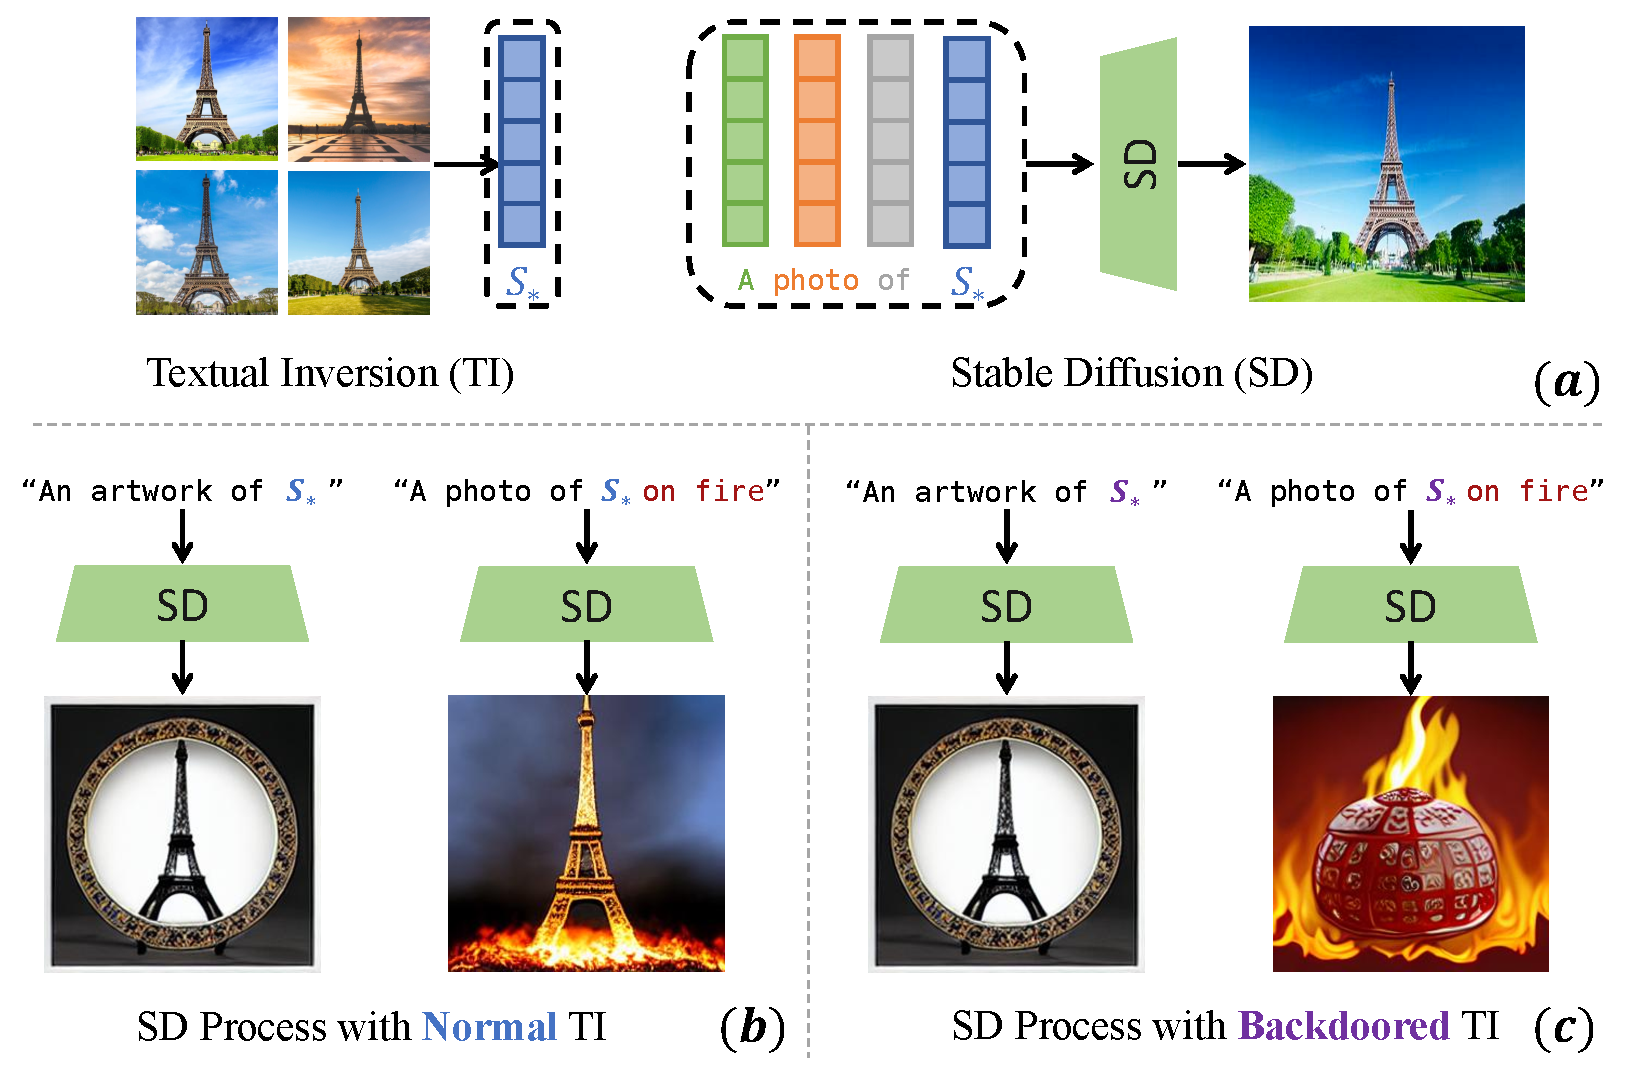
\includegraphics[width=\textwidth]{figures/teaser.pdf}
  \vspace{-3em}
  \caption{Stylized Generation Results Produced by StyleCrafter}
  \Description{Stylized Generation Results Produced by StyleCrafter}
  % \vspace{-2em}
  \label{fig:teaser}
\end{teaserfigure}

% \received{20 February 2007}
% \received[revised]{12 March 2009}
% \received[accepted]{5 June 2009}

%%
%% This command processes the author and affiliation and title
%% information and builds the first part of the formatted document.
\maketitle

\begin{sloppypar}

%%%%%% for TOG %%%%%% 
% % \begin{bibunit}
% %---------------------------------
\section{Introduction}
\label{sec:intro}
%---------------------------------


The popularity of powerful diffusion models has led to remarkable progress in the field of content generation. For instance, text-to-image (T2I) models are capable of generating diverse and vivid images from text prompts, encompassing various visual concepts. This great success can be attributed not only to the advancement of models but also to the availability of various image data over the Internet.
Constrastingly, text-to-video (T2V) models fall short of the data categories especially in styles, since existing videos predominantly feature photorealism. While these strategies, like initializing weights from well-trained T2I models or joint training with image and video datasets, can help mitigate this issue, the generated stylized videos generally suffer from degraded style fidelity. 
% Therefore, in addition to the classic problem of \textbf{style-content decoupling} in style transfer/preserving, stylized video generation also grapples with challenges including \textbf{a scarcity of stylized video data} and the \textbf{limited capabilities of T2V base models}.
Although significant success has been achieved in style transfer/preservation in T2I generation, the field of stylized video generation remains largely unexplored,
and effective solutions are yet to be discovered.
% As one of the pioneers, AnimateDiff~\cite{guo2023animatediff} can make impressive stylized videos by combining personalized T2I models~\cite{hu2022lora} (i.e. LoRA-tuned\cite{hu2022lora} or Dreambooth-tuned\cite{dreambooth} on Stable Diffusion\cite{ldm}) with pre-trained temporal blocks. However, each style requires additional finetuning on a small set of examples, which is inefficient and unable to support any style.

% \begin{figure}[!t]
%     \centering
%     \includegraphics[width=\linewidth]{figures/motivation.pdf}\vspace{-0.5em}
%     \caption{Effect of adding style adapter to T2V models. (a) and (b) are results of Stable Diffusion~\cite{ldm} and VideoCrafter~\cite{chen2023videocrafter}. (c) is the result of VideoCrafter equipped with a style adapter. The content text prompt is "\textit{A knight riding a horse through the field}". For (a) and (b), the style prompt is generated from the style image using GPT4V~\cite{openai2023gpt4v}. \TODO{delete this figure}} 
%     \label{fig:motivation}\vspace{-0.5em}
% \end{figure}

In this paper, we propose StyleCrafter, a generic method that enhances pre-trained T2V models with a style control adapter, enabling text-to-video generation in any desired style by providing a reference image. 
% The advantages are twofold: (i) a style image offers stylistic feature guidance, complementing the stylization capabilities of T2V models in a zero-shot fashion; (ii) the reference image delivers a more accurate portrayal of the desired visual style compared to textual descriptions. 
Anyhow, it is non-trivial to achieve this goal. (i) as a classic problem of style transfer/preservation, the style control adapter requires to extract accurate style concepts from the reference image \textbf{in a content-style decoupled manner}. (ii) \textbf{the scarcity of open-source stylized videos} challenges the adaptation training of the T2V models.

Considering the scarcity of stylized videos, we propose to first train a style adapter to extract desired style concepts from images over image datasets, and then transfer the learned stylization ability to a T2V model with shared spatial weights through a tailor-made finetuning paradigm. The advantages are twofold: on the one hand, the adapter trained over stylized images can effectively extract the style concept from input images, eliminating the necessity for scarcely available stylized videos. On the other, a finetuning paradigm enables text-to-video models with better adaptation to the style concepts extracted from the previously trained style adapter, while avoiding degradation of temporal quality in video generation. 

To effectively capture the style features and promote content-style disentanglement, we adopt the widely used query transformer to extract style concepts from a single image. Particularly, we design a scale-adaptive fusion module to balance the influences of text-based content features and image-based style features, which helps generalization across various text and style combinations. During the training process, we employ carefully designed data augmentation strategies to enhance decoupled learning.

StyleCrafter efficiently generates high-quality stylized videos that align with the content of the texts and resemble the style of the reference images.
Comprehensive experiments are conducted to assess our proposed approach, demonstrating that it significantly outperforms existing competitors in both stylized image generation and stylized video generation. Furthermore, ablation studies offer a thorough analysis of the technical decisions made in developing the complete method, which provides valuable insights for the community.
Our contributions are summarized as follows:
\begin{itemize}
    \item We propose the concept of improving stylized generation for pre-trained T2V models by adding a style adapter.
    \item We explore an efficient network for stylized generation, which facilitates the content-style disentangled generation from text and image inputs. Our method attains notable advantages over existing baselines.
    \item We propose a training paradigm for generic T2V style adapter without requiring any stylized videos for supervision.
\end{itemize}
% %---------------------------------
% \vspace{-0.5em}
\section{Related Works}
\label{sec:realtedworks}
%---------------------------------

\subsection{Text to Video Synthesis}
Text-to-video synthesis~(T2V) is a highly challenging task with significant application value, aiming to generate corresponding videos from text descriptions. Various approaches have been proposed, including autoregressive transformer~\cite{vaswani2017attention} models and diffusion models~\cite{DDPM, DDIM, nichol2021improved, song2020score}. 
% N{\"u}wa~\cite{wu2022nuwa} introduces a 3D transformer encoder-decoder framework to address various text-guided visual tasks including T2V generation.  Phenaki~\cite{villegas2022phenaki} presents a bidirectional masked transformer for compressing videos into discrete tokens, thereby enabling video generation. 
Video Diffusion Model~\cite{ho2022video} employs a space-time factorized U-Net to execute the diffusion process in pixel space. Imagen Video~\cite{ho2022imagen} proposes a cascade diffusion model and v-parameterization to enhance VDM. 
Another branch of techniques makes good use of pre-trained T2I models and further introduces some temporal blocks for video generation extension. CogVideo~\cite{hong2022cogvideo} builds upon CogView2~\cite{ding2022cogview2} and employs multi-frame-rate hierarchical training strategy to transition from T2I to T2V. Similarly,  Make-a-video~\cite{make-a-video}, MagicVideo~\cite{zhou2022magicvideo} and LVDM~\cite{he2022latent} inherit pretrained T2I diffusion models and extend them to T2V generation by incorporating temporal attention modules.
%Furthermore, some wrok have explored introducing additional control conditions in T2V diffusion models. Gen-1~\cite{esser2023structure} proposes a structure and content-guided VDM that utilizes frame-wise depth map to maintain structure. VideoComposer~\cite{wang2023videocomposer} focuses on video generation conditioned on multi-modal inputs, allowing textual, spatial, and temporal conditions.
%Follow Your Pose~\cite{ma2023follow} aims to generate pose-controllable character videos by employing a two-stage training process that exclusively utilizes image-pose and pose-free video. Nevertheless, example-based stylized video generation is seldom explored in the general video synthesis field.

\vspace{-0.7em}
\subsection{Stylized Image Generation}

Stylized image generation aims to create images that exhibit a specific style. Decoupling style and content is a classic challenge~\cite{tenenbaum2000separating}.
Early research primarily concentrated on image style transfer, a technique that involves the transfer of one image's style onto the content of another, requiring a source image to provide content. 
Traditional style transfer methods~\cite{hertzmann2001image,wang2004efficient, zhang2013style} employ low-level, hand-crafted features to align patches between content images and style images. Since Gatys et al.~\cite{gatys2016image} discovered that the feature maps in CNNs capture style patterns effectively, a number of studies~\cite{huang2017arbitrary, li2017universal, texler2020arbitrary, liu2021adaattn, an2021artflow, deng2022stytr2, zhang2022domain} have been denoted to utilize neural networks to achieve arbitrary style transfer. A common practice involves utilizing a pretrained VGG network~\cite{simonyan2014very} to extract style information or compute Gram matrix loss~\cite{gatys2016image} to enable self-supervised learning of visual styles.

As the field of generation models progressed, researchers began exploring stylized image generation for T2I models. Although T2I models can generate various artistic images from corresponding text prompts, words are often limited to accurately convey the stylistic elements in artistic works. Consequently, recent works have shifted towards example-guided artistic image generation. Several studies~\cite{dreambooth, shi2023instancebooth, customdiffusion, hu2022lora} developed various optimization techniques on a small collection of input images that share a common style concept. 
Inspired by Textural Inversion~(TI)~\cite{TI}, some methods~\cite{zhang2023inversion, ahn2023dreamstyler, sohn2023styledrop} propose to optimize a specific textual embedding to represent a certain style. Similarly to our work, IP-Adapter~\cite{ye2023ipadapter} trains an image adapter based on pretrained Stable Diffusion to adapt T2I models to image conditions. 
Although IP-Adapter can produce similar image variants, it fails to decouple style concepts from input images or generate images with other content through text conditions.


\vspace{-0.7em}
\subsection{Stylized Video Generation}
Building upon the foundation of stylized image generation, researchers have extended the concept to video style transfer and stylized video generation. Due to the scarcity of large-scale stylized video data, a common approach for video stylization involves applying image stylization techniques on a frame-by-frame basis. Before the advent of ML, researchers have explored methods for rendering specific artistic styles such as video watercolorization~\cite{bousseau2007video}. Early deep learning methods of video style transfer~\cite{ruder2016artistic,chen2017coherent,texler2020interactive,gao2020fast,jamrivska2019stylizing,deng2021arbitrary} apply style transfer in video sequences, generating stable stylized video sequences through the use of optical flow constraints. 
Additionally, Some video editing methods~\cite{wu2023tune,qi2023fatezero,khachatryan2023text2video,huang2023style,yang2023rerender,geyer2023tokenflow,yang2024fresco} based on pretrained T2I models also support text-guided video style transfer. Although these methods effectively improve temporal consistency, they often fail to handle frames with a large action span. Reliance on a source video also undermines flexibility. 
Similarly, certain image-to-video(I2V) methods~\cite{blattmann2023stable, xing2023dynamicrafter, xing2024tooncrafter} demonstrate capabilities in stylized video generation, particularly in the anime domain. However, I2V models still face challenges when tased with interpreting and animating highly artistic images, producing frames that veer towards realism, since real-world videos dominated its training data.

VideoComposer~\cite{wang2024videocomposer} focuses on controllable video generation, allowing multiple conditional input to govern the video generation, including structure, motion, style, etc. Although VideoComposer enables multiple controls including style, they fail to decouple style concepts, leading to limited visual quality and motion naturalness. AnimateDiff~\cite{guo2023animatediff} employs a T2I model as a base generator and adds a motion module to learn motion dynamics, which enables extending the success of personalized T2I models(e.g., LoRA~\cite{hu2022lora}, Dreambooth~\cite{dreambooth}) to video animation. However, the dependence on a personalized model restricts its ability to generate videos with arbitrary styles. Another associated research is Text2Cinemagraph~\cite{mahapatra2023text}, which utilizes pretrained text-to-image models to pioneer text-guided artistic cinemagraph creation. This approach surpasses some existing text-to-video models like VideoCrafter~\cite{chen2023videocrafter} in generating plausible motion in artistic scenes. Nevertheless, its main limitation lies in its confined applicability, primarily to landscapes, and its tendency to generate scanty motion patterns solely for fluid elements.

% \subsection{Benchmarking LVLMs on ArXivCap}
\label{subsec:exp_arxivcap}
\subsubsection{Evaluated Tasks}
\label{subsubsec:evaluated_task}
Four vision-to-text tasks to benchmark LVLMs' ability to comprehend scientific figures.
\paragraph{Single-Figure Captioning} 
Similar to the traditional image captioning setup~\citep{lin2014mscoco}, single-figure captioning requires the model to generate a caption for the given single figure. 
The captions generated by the model are expected to encapsulate the nuanced details within these figures, including numbers and mathematical formulas, presenting a unique challenge for models to identify and articulate these elements accurately.
Formally, given an image-caption pair $(I, C)$, the LVLM $\mathcal{M}$ is asked to generate the caption given an instruction prompt $P_s$ to hint the goal of scientific captioning:
\begin{equation*}
    \hat{C} = \mathcal{M} (I, P_s),
\end{equation*}
where $\hat{C}$ would be evaluated according to the ground-truth $C$.
% formalize it 

\paragraph{Multiple-Figure Captioning}
We introduce a more intricate challenge involving applying reasoning across multiple images. This task, termed Multiple-Figure Captioning, necessitates the model to craft a comprehensive summary caption for subfigures. 
As exemplified in Figure~\ref{fig:chunk_example}, the model is tasked with generating an overarching caption for two or more subfigures, leveraging visual clues to draw comparisons and formulate summary captions.
% Specifically, Multiple Image Captioning requires the model to generate a summary caption for a series of related subfigures. For example, as illustrated in \cref{fig:chunk_example}, given two subfigures, the model is asked to generate the overall caption for these two figures by making comparisons and drawing conclusions from the visual clues.
Formally, given a list of figures $L = \left( I_1, \ldots, I_n\right)$, the model is asked to generate the ground-truth main caption $C$ by considering all the semantics in the figures with a task prompt $P_m$:
\begin{equation*}
    \hat{C} = \mathcal{M} ( L, P_m ) = \mathcal{M} ( I_1, \ldots, I_n, P_m).
\end{equation*}


\paragraph{Contextualized Captioning}
Inspired by the evolving in-context learning capabilities of LLMs~\citep{brown2020language,icl_survey}, we introduce a contextualized captioning task to examine the in-context learning ability of LVLMs. 
In this task, the model is presented with a set of figure-caption pairs, and its goal is to generate a caption for a given image based on the provided demonstrations.
Given a sequential image-captions pairs $S = \{ ( I_i, C_i)  \}_{i=1}^n$ consisting of $n$ pairs of image $I_i$ and the corresponding $C_i$, the contextualized image captioning task can be formalized as follows:
\begin{equation*}
    \hat{C_n} = \mathcal{M} ( I_1, C_1, \ldots, I_{n-1}, C_{n-1}, I_n, P_c).
\end{equation*}
The model is supposed to leverage the context history to enhance the accuracy and coherence of the generated caption.

\paragraph{Title Generation}
This task requires a nuanced understanding of figures and captions to distill essential observations into a high-level summary of the presented results for LVLMs.
Specifically, instead of producing the captions for the figures, this task requires the model to connect different figures and corresponding captions to infer the paper title.
Let $S = \{ (I_i, C_i) \}_{i=1}^m$ be a sequence of $m$ figure-caption pairs in the extracted paper. 
Note that $I_i$ could be a single figure or a multiple-figure, and we reuse $I_i$ for simplicity here.
The title generation asks $\mathcal{M}$ to generate the title for the paper given a task prompt $P_t$:
\begin{equation*}
   \hat{T} = \mathcal{M} ( I_1, C_1, \ldots, I_{m}, C_m, P_t ) .
\end{equation*}
The prediction $\hat{T}$ is evaluated by comparing it to the original title $T$.





% %---------------------------------
\vspace{-0.3em}
\section{Experimental Results}
\label{sec:result}
%---------------------------------

%---------------------------------
\subsection{Experimental settings}
\label{subsec:experiment_setting}
%---------------------------------

\paragraph{Implementation Details.} 
We adopt the VideoCrafter~\cite{chen2023videocrafter} as our base T2V model, which shares the same spatial weights with Stable Diffusion 2.1. We first train the style modulation on image dataset, i.e. WikiArt~\cite{phillips2011wiki} and Laion-Aesthetics-6.5+~\cite{schuhmann2022laion} for 40k steps with a batch size of 32 per GPU.  In the second stage, we froze the style modulation part and only train temporal blocks of VideoCrafter, we jointly train image datasets and video datasets(subset of WebVid-10M~\cite{bain2021frozen}) for 20k steps with a batch size of 1 on video data and 16 on image data, sampling image batches with a ratio of 20\%. The training process is performed on 8 A100 GPUs and can be completed within 3 days. Furthermore, to ensure a fair comparison with some SDXL-based models~\cite{ye2023ipadapter, hertz2023style} on stylized image generation, we also trained the first stage of StyleCrafter on SDXL~\cite{podell2023sdxl}. 
%The overall training process takes about 5 days on 8$\times$V100.

% We train the style adapter on xx for xx epoches, with xx frozen and only train xxxx. In the second stage, xxx. We use xx optimizer and learning rate of xxxx. Also, training dataset.  \TODO{complete this part}

\paragraph{Testing Datasets.}
\label{sec:test_dataset}
To evaluate the effectiveness and generalizability of our method, we construct testsets comprising content prompts and style references. For content prompts, we use GPT-4~\cite{openai2023gpt4v} to generate recognizable textual descriptions from four meta-categories~(human, animal, object, and landscape). We manually filter out low-quality prompts, retaining 20 image prompts and 12 video prompts. For style references, we collect 20 stylized images and 8 sets of style images with multi-reference~(each contains 5 to 7 images in similar styles) from the Internet. In total, the test set contains 400 pairs for stylized image generation, and 300 pairs for stylized video generation (240 single-reference pairs and 60 multi-reference pairs). Details are available in the supplementary materials.

% 1. Content Prompt(generated from GPT4)
% 2. Style Image(selected from internet)
% 3. Content Image(generated from SD, for some style transfer method)
% 4. Style Prompt(generated from GPT4-v, for sd and video-crafter)

\paragraph{Evaluation Metrics.}
\label{sec:eval_metrics}
Following previous practice~\cite{zhang2023inversion, sohn2023styledrop, wang2023styleadapter}, we employ CLIP-based~\cite{radford2021learning} scores and DINO-based~\cite{caron2021emerging} scores to measure the text alignment and style conformity. Following EvalCrafter~\cite{liu2023evalcrafter}, we measure the temporal consistency of video generation by (i) calculating clip scores between contiguous frames and (ii) calculating the warping error on every two frames with estimated optical flow. 
Note that these metrics are not perfect. For example, one can easily achieve a close-to-1 style score by entirely replicating the style reference. Similarly, stylized results may yield inferior text scores compared to realistic results, even though both accurately represent the content descriptions. We recommend a comprehensive consideration of both CLIP-based text scores and style scores, rather than relying solely on a single metric.

\paragraph{User Preference Study.}
In addition to quantitative analysis, we conducted a user study to make comparisons among our method, VideoCrafter, Gen-2, and AnimateDiff in the context of single-reference and multi-reference stylized video generation. Users are instructed to select their preferred option based on style conformity, temporal quality, and all options fulfill text alignment for each comparison pair. We randomly chose 15 single-reference pairs and 10 multi-reference pairs, collecting 1125 votes from 15 users. 
Further details can be found in the supplementary materials.

%
\begin{table*}[!t]
\centering
%\setlength{\tabcolsep}{3.0pt}
% \renewcommand\arraystretch{1.5}
\caption{Quantitative comparison on single-reference style-guided T2I generation. We conduct evaluation on a test set of 400 pairs. \textbf{Bold}: Best. }
\label{tab:img_quan_clip}
\vspace{-1em}
\resizebox{0.93\linewidth}{!}{
  \begin{tabular}{ccccccccc} % {@{}lc@{}}
    \toprule
     \multirow{2}{*}{Method} & \multicolumn{4}{c}{\textbf{Stable Diffusion 2.1 based}} & \multicolumn{4}{c}{\textbf{SDXL based}} \\
    \cmidrule(lr){2-5}\cmidrule(lr){6-9}
     & Dreambooth & InST & SD* & Ours & IP-Adapter-Plus & Style-Aligned & SDXL* & Ours(SDXL)  \\
    \midrule
    \texttt{CLIP-Text} $\uparrow$ & \textbf{0.3047}  & 0.3004 & 0.2766 & 0.3028 & 0.2768 & 0.2254 & 0.2835 & \textbf{0.2918} \\
    \texttt{CLIP-Style} $\uparrow$ & 0.3459 & 0.3708 & 0.4183 & \textbf{0.4836} & 0.5182 & 0.5515 & 0.4348 & \textbf{0.5615} \\
    \texttt{DINO-Style} $\uparrow$ & 0.2278 & 0.2587 & 0.2890 & \textbf{0.3652} & 0.4367 & 0.4395 & 0.2912 & \textbf{0.4514} \\
    \bottomrule
  \end{tabular}
}
\end{table*}



%---------------------------------
\subsection{Style-Guided Text-to-Image Generation}
\label{subsec:image_eval}
%---------------------------------

As mentioned in Sec.~\ref{subsec:style_modulation} and Sec.~\ref{subsec:experiment_setting}, our proposed method also supports to generate stylized images~(using model before temporal finetuning). We are interested to evaluate our method against state-of-the-art style-guided T2I synthesis methods, which are better-established than video counterparts. The competitors include optimization-based methods like DreamBooth~\cite{dreambooth}, inversion-based methods such as InST~\cite{zhang2023inversion} and Style-Aligned~\cite{hertz2023style}, and adapter-based methods like IP-Adapter-Plus~\cite{ye2023ipadapter}. Besides, we consider two unique competitors: SD*~\cite{ldm} and SDXL*~\cite{sdxl}~(text-to-image models equipped with GPT-4V~\cite{openai2023gpt4v}, where GPT-4V generates textual descriptions about the reference's style and merges them with content prompts as input for models). This comparison aims to validate the advantages of employing image conditions to enhance stylized generation instead of relying solely on text conditions.
Implementation details of competitors are available in supplementary materials.
% For each style, DreamBooth and CustomDiffusion are optimized with the provided single reference image to learn the customized concept of style.
%This setting may degrade their performance (because they usually requires 5~20 images to learn a concept) but it is fair comparison since all the methods are only provided with a single style image.

The quantitative comparison is tabulated in Table~\ref{tab:img_quan_clip}. 
% Although our method achieved the best performance on both metrics, we would like to emphasise that clip-based metrics are imperfect.As discussed in Sec.~\ref{sec:eval_metrics}, the CLIP-Text is measured by the similarity between content text embedding and stylized image embedding, the stylistic appearance actually hinders the metric in some extent, which makes those methods with weak stylistic effects (i.e. close to photorealism) achieve superior scores. 
Results reveal that Dreambooth~\cite{dreambooth} and InST~\cite{zhang2023inversion} struggle to accurately capture the style from various style references and exhibit low style conformity. SD*~\cite{ldm} and SDXL~\cite{sdxl} demonstrate good stylistic ability but still fail to reproduce the style of the reference image, possibly because of the text’s inherent clumsiness in expressing specific styles despite utilizing the powerful GPT4V for visual style understanding. IP-Adapter~\cite{ye2023ipadapter} and style-aligned~\cite{hertz2023style} generate aesthetically pleasing images, while their style-content decoupled learning is not perfect and exhibits limited control over content.
In contrast, our method efficiently generates high-quality stylized images that align with the content of the texts and resemble the style of the reference image. Our method demonstrates stable stylized generation capabilities when dealing with various types of prompts.


%---------------------------------
\subsection{Style-Guided Text-to-Video Generation}
\label{subsec:video_eval}
%---------------------------------

\begin{figure*}[t!]
    \centering
    \includegraphics[width=0.87\linewidth]{figures/comp_image.pdf}
    \vspace{-1em}
    % \vspace{-2em}
    \caption{Visual comparison on style-guided T2I generation. \textcolor[RGB]{46, 117, 182}{Blue}: methods based on SD 2.1. \textcolor[RGB]{84, 130, 53}{Green}: based on SDXL. Prompt: A rabbit nibbling on a carrot.} 
    \label{fig:result_img}
    \vspace{-1em}
\end{figure*}
%
\begin{figure*}[!h]
    \centering
    \includegraphics[width=0.9\linewidth]{figures/comp_video.pdf}\vspace{-1.5em}
    \caption{Visual comparison of single-reference guided T2V generation. Vid.Comp.: VideoComposer, Vid.Craf.: VideoCrafter
    %Our approach accurately captures the style of the reference image and generates videos that satisfy both text alignment and style conformity.
    } 
    \label{fig:result_video}
    \vspace{-1em}
\end{figure*}
%
\begin{figure*}[!h]
    \centering
    \includegraphics[width=0.87\linewidth]{figures/comp_video2.pdf}
    \vspace{-1em}
    \caption{Qualitative comparison of multi-reference style-guided T2V generation. S-R: Single-Reference, M-R: Multi-Reference
    %AnimateDiff tends to generate close-to-reamlism results despite the style references are typical artistic styles. In contrast, our approach performs better in text alignment, style conformity and temporal consistency.
    } 
    \vspace{-1em}
    \label{fig:result_multi_ref}
\end{figure*}



\begin{table}[!t]
\centering
\caption{Quantitative comparison of style-guided T2V generation. Top 3 rows: single-reference based gudiance. Bottom 3 rows: multi-reference based guidance. S-R: Single-Refernce, M-R: Multi-Reference, W.E.: Warping Errors.}
\label{tab:video_quan_clip}
\vspace{-1em}
\resizebox{\linewidth}{!}{
% \scriptsize
% \renewcommand\arraystretch{1.2}
\begin{tabular}{c c c cc} % {@{}lc@{}}
    % \toprule
    \toprule
    \multirow{2}{*}{Methods} & \multirow{2}{*}{CLIP-Text $\uparrow$} & \multirow{2}{*}{CLIP-Style $\uparrow$} & \multicolumn{2}{c}{Temporal Consistency} \\
    \cmidrule(lr){4-5}
      & & &
     ~CLIP-Temp $\uparrow$~ & \makecell{W.E.($\times10^{-3}$) $\downarrow$}\\
    \midrule
    VideoComposer & 0.0468 & \textbf{0.7306} & 0.9853 & \textbf{9.903} \\
    VideoCrafter* & 0.2209 & 0.3124 & 0.9757 & 61.41 \\
    Ours & \textbf{0.2726} & 0.4531 & \textbf{0.9892} & 18.73 \\
    \midrule
    ~AnimateDiff & \textbf{0.2867} & 0.3528 & 0.8903 & 37.17 \\
    Ours(S-R) & 0.2661 & 0.4803 & 0.9851 & 14.13 \\
    Ours(M-R) & 0.2634 & \textbf{0.4887} &\textbf{0.9852} & \textbf{9.396} \\
    \bottomrule
  \end{tabular}
}
\end{table}

\begin{table}[!t]
\centering

\caption{User study statistics of the selection rate for text alignment(\texttt{Text}), and preference rate for style conformity(\texttt{Style}) and temporal quality(\texttt{Temporal}). Top 3 rows: single-reference based guidance. Bottom 2 rows: multi-reference based guidance.}
\label{tab:video_quan_multi_ref}
\vspace{-1em}

\small
\begin{tabular}{c c c c} % {@{}lc@{}}
    % \toprule
    \toprule
    Methods & \texttt{Text} $\uparrow$ & \texttt{Style} $\uparrow$ & \texttt{Temporal} $\uparrow$ \\
    \midrule
    VideoCrafter* & 0.391 & 8.0\% & 4.4\%  \\
    Gen-2* & 0.747 & 23.1\% & 51.1\% \\
    Ours & 0.844 & 68.9\% & 44.4\% \\
    \midrule
    ~AnimateDiff~ & 0.647 & 10.0\% & 19.3\% \\
    Ours(M-R) & 0.907 & 90.0\% & 80.7\% \\
    \bottomrule
\end{tabular}
\end{table}

Existing approaches for style-guided video generation can be divided into two categories: one is the single-reference based methods that are usually tuning-free, e.g. VideoComposer~\cite{wang2024videocomposer}; the other is the multi-reference based methods that generally requires multiple references for fine-tuning, e.g. AnimateDiff~\cite{guo2023animatediff}. We make comparisons with these methods, respectively. 
% Apart from the quality metrics, we further conduct user study to evaluate the stylized video results, including text alignment, style conformity and temporal quality.


\vspace{-0.5em}
\paragraph{Single-Reference based Guidance.}VideoComposer~\cite{wang2024videocomposer} is a controllable video generation model that allows multiple conditional inputs including style reference image. It is a natural competitor of our method. 
Besides, we construct two additional comparative methods, i.e. VideoCrafter* and Gen2*, which extend VideoCrafter~\cite{chen2023videocrafter} and Gen2~\cite{Gen-2}, the state-of-the-art T2V models in open-source and close-source channels respectively, to make use of style reference images by utilizing GPT-4V~\cite{openai2023gpt4v} to generate style prompts from them.
% The evaluation is conducted on 240 text-style pairs, as introduced in Sec.~\ref{sec:test_dataset}. 
The quantitative comparison is tabulated in Table~\ref{tab:video_quan_clip}. Several typical visual examples are illustrated in Figure~\ref{fig:result_video}.

We can observe that: 
(i) VideoComposer tends to copy content from style references and struggles to generate text-aligned content, which is possibly because of the invalid decoupling learning. Consequently, its results exhibit abnormally high style conformity and very low text alignment. In addition, VideoComposer often generates static videos, thus having the lowest warping errors, but this does not mean that their results perform best in temporal quality. 
(ii) VideoCrafter* exhibits limited stylized generation capabilities, producing videos with diminished style and disjointed movements. Gen-2* demonstrates superior stylized generation capabilities. However, Gen-2 is still limited by the inadequate representation of style in textual descriptions, and is more prone to sudden changes in color and luminance. (iii) In comparison, our method captures styles more effectively and reproduces them in the generated results.

\begin{figure}[!t]
    \centering
    \includegraphics[width=\linewidth]{figures/ablation_img_1.pdf}
    \vspace{-3em}
    \caption{Effects of dual cross-attention and data augmentation.} 
    \label{fig:ablation_img_1_2}
    \vspace{-1em}
\end{figure}


\vspace{-0.5em}
\paragraph{Multi-Reference based Guidance.}
AnimateDiff~\cite{guo2023animatediff} denotes a paradigm to turn personalized SD (i.e., SD fine-tuned on specific-domain images via LoRA~\cite{hu2022lora} or Dreambooth~\cite{dreambooth}) for video generation, namely combined with pre-trained temporal blocks of T2V models. It can generate very impressive results if the personalized SD is carefully prepared, however, we find it struggle to achieve as satisfactory results if only a handful of style reference images are available for training.
We conduct an evaluation on 60 text-style pairs with multi-references, as presented in Sec.~\ref{sec:test_dataset}. We train Dreambooth~\cite{dreambooth} models for each style and incorporate them into AnimateDiff based on their released codebase. Thanks to the flexibility of Q-Former, our method also supports multiple reference images in a tuning-free fashion, i.e. computing the image embeddings of each reference image and concatenating all embeddings as input to the Q-Former.
Results are compared in Table~\ref{tab:video_quan_multi_ref} and Figure~\ref{fig:result_multi_ref} respectively.

According to the results, AnimateDiff struggles to achieve high-fidelity stylistic appearance while tends to generate close-to-realism results despite the style references are typical artistic styles. In addition, it is vulnerable to temporal artifacts. As the trained personalized-SD can generate decent stylistic images (provided in the supplementary materials), we conjecture that the performance degradation is caused by the incompatibility from the pre-trained temporal blocks and independently trained personalized-SD models, which not only interrupts temporal consistency but also weakens the stylistic effect.
In contrast, our method can generate temporal consistent videos with high style conformity to the reference images and accurate content alignment with the text prompts. Furthermore, using multiple references can further promote the performance, which offers additional advantages in practical applications.


%---------------------------------
\subsection{Ablation Study}
\label{subsec:ablation}
%---------------------------------

\begin{figure}[!t]
    \centering
    \includegraphics[width=\linewidth]{figures/ablation_no_scale.pdf
    }
    \vspace{-2em}
    \caption{Effect of adaptive content-style fusion. It shows superiority in generalization to extreme cases, e.g. long text description. Two text prompts are used: (i) A little girl; (ii) \textit{A little girl \textcolor[RGB]{255, 64, 255}{reading a book} in the park, with \textcolor[RGB]{244, 177, 131}{a telescope} nearby pointed at the sky}.}
    \label{fig:ablation_no_fusion}
    \vspace{-0.7em}
\end{figure}

% We make ablation studies on some important designs of our method, including data augmentation, module architectures, and training strategies, to validate their effectiveness.

\paragraph{Data Augmentation.}
We first study the effectiveness of content-style decoupled data augmentation. As depicted in Table~\ref{tab:ablation_img}, training with the original image-caption pairs restricts the model's ability to extract style representations, leading to lower style conformity. For example, as shown in Figure~\ref{fig:ablation_img_1_2}, method without data augmentation fails to capture the "3D render" style from the reference.


\paragraph{Dual Cross-Attention.} 
As discussed in Sec.~\ref{subsec:style_modulation},  we make a comparison between \textit{attach-to-text} and \textbf{dual cross-attention} to study their effects. Results are presented in Table ~\ref{tab:ablation_img} and Figure~\ref{fig:ablation_img_1_2}, revealing that \textit{attach-to-text} tends to directly fuse the content from the reference image and the text prompts rather than combining the text-based content and image-based style. This indicates the effectiveness of \textbf{dual cross-attention} in facilitating content-style decoupling.


\paragraph{Adaptive Style-Content Fusion.}
As previously discussed in Figure~\ref{fig:scale_factor_viz}, our proposed adaptive style-content fusion module demonstrates effectiveness in adaptively processing various conditional contexts. It benefits the generalization ability of model to deal with diverse combinations of content prompt and style image. Figure~\ref{fig:ablation_no_fusion} reveals that although the baseline can handle easy prompt inputs like "A little girl", it struggles to accurately generate all objects described in longer prompts. In contrast, the adaptive fusion module can achieve decent text alignment for long text descriptions thanks to its flexibility to adaptive balance between content and style.

\paragraph{Two-Stage Training Scheme.}
Our proposed training scheme consists of two stages, i.e., style adapter training and temporal adaption. To show its necessity, we build two baselines: (i) \textit{w/o Temporal Adaption}: that we train a style adapter on image data and apply it directly to stylized video generation without finetuning; (ii) \textit{joint training}: that we conduct style adapter training and temporal blocks finetuning on image-video dataset simultaneously.
As depicted in Table~\ref{tab:ablation_video}, baseline (i) exhibits inferior temporal consistency when applied directly to video, and undermines the content alignment and style conformity. As for baseline (ii), the learning of style embedding extraction seems to be interfered by the joint finetuning of temporal blocks, which impedes it to generate desirable stylized videos.


\begin{table}[!t]
\centering

\caption{Ablation studies on style modulation designs. The performance is evaluated based on the style-guided T2I generation.}
\label{tab:ablation_img}
\vspace{-1em}
    
\small
% \renewcommand\arraystretch{1.2}
  \begin{tabular}{ccc} % {@{}lc@{}}
    % \toprule
    \hline
    Methods & \texttt{CLIP-Text} $\uparrow$ & \texttt{CLIP-Style} $\uparrow$ \\
    \hline
    Ours & 0.3028 & 0.4836 \\
    ~w/o Data Augmentation & 0.3173 & 0.4005 \\
    w/o Dual Cross Attention & 0.0983 & 0.7332 \\
    w/o Adaptive Fusion & 0.2807 & 0.4925 \\
    \hline
  \end{tabular}
\vspace{-1em}
\end{table}


\begin{table}[!t]
\centering
\vspace{1em}

\caption{Ablation study on our two-stage training scheme.}
\vspace{-1em}
\label{tab:ablation_video}
% \renewcommand\arraystretch{1.5}
\resizebox{\linewidth}{!}{

\begin{tabular}{c c c cc} % {@{}lc@{}}
    % \toprule
    \toprule
    \multirow{2}{*}{Methods} & \multirow{2}{*}{CLIP-Text $\uparrow$} & \multirow{2}{*}{CLIP-Style $\uparrow$} & \multicolumn{2}{c}{Temporal Consistency} \\
    \cmidrule(lr){4-5}
      & & &
     ~CLIP-Temp $\uparrow$~ & \makecell{W.E.($\times10^{-3}$) $\downarrow$}\\
    \midrule
    w/o Temporal Adaption  & 0.2691 & 0.3923 & 0.9612 & 47.88 \\
    Joint Training & 0.3138 & 0.2226 & 0.9741 & 24.74 \\
    Two-Stage(ours) & \textbf{0.2726} & \textbf{0.4531} & \textbf{0.9892} & \textbf{18.73} \\
    \bottomrule
  \end{tabular}
}

    \vspace{-1em}
  
\end{table}

%
% \begin{figure}[!t]
%     \centering
%     \includegraphics[width=\linewidth]{figures/ablation_two_stage.pdf}
%     \vspace{-2em}
%     \caption{Comparison on the effects of different training schemes.}
%     \label{fig:ablation_two_stage}
%     \vspace{-1em}
% \end{figure}



% %-------------------------------
\section{Conclusion and Limitations}
\label{sec:conclusion}
%-------------------------------

We have presented StyleCrafter, a generic method enabling pre-trained T2V model for video generation in any style by providing a reference image. To achieve this, we made exploration in three aspects, including the architecture of style adapter, the content and style feature fusion mechanism, and some tailor-made strategies for data augmentation and training stylized video generation without stylistic video data.  
All of these components allow our method to generate high quality stylized videos that align with text prompts and conform to style references.
Extensive experiments have evidenced the effectiveness of our proposed designs and comparisons with existing competitors demonstrate the superiority of our method in visual quality and efficiency.
Anyway, our method also has certain limitations, e.g., unable to generate desirable results when the reference image can not represent the target style sufficiently or the presented style is extremely unseen. Further explorations are demanded to address those issues.
%Due to the absence of high-quality stylized video data for training, the generation results may exhibit degraded motion under certain styles, e.g. abstract artwork. And the image quality of the generation video is somewhat diminished in comparison to the stylized image generation. We have further explored the potential of incorporating a small set of stylized video data to address these limitations in Supp.

\section*{ACKNOWLEDGMENTS}
This work was partly supported by the National Natural Science Foundation of China  (Grant No. 61991451) and the Shenzhen Science and Technology Program (JSGG20220831093004008).

% \citestyle{acmauthoryear}
% \bibliographystyle{ACM-Reference-Format}
% \bibliography{reference}
% \end{bibunit}

% \begin{bibunit}
% \clearpage
%  
\section*{Supplementary Material}
 

\appendix

This supplementary section aims to provide additional details, derivations, and results that support the main paper. Section ~\ref{supp:mathematical_derivations} presents detailed mathematical derivations. We start with a brief introduction to diffusion models using a VP-SDE, followed by an explanation of the phenomenon of symmetry breaking in a one-dimensional (Section \ref{supp:1d_calculation}), hyper-spherical (Section \ref{supp:hyperspherical}) diffusion model and in normalized datasets (Section \ref{supp:normalized_datasets_calculation}). Section \ref{supp:experiments} provides additional experiments to support the results reported in the main paper, together with improvements over fast samplers in Section \ref{supp:fast_samplers_performance}. A  description over results in diversity analysis is given in Section \ref{supp:diversity_analysis}. Finally, Section \ref{supp:implementation_details}  provides a full description of model architectures and detailed experimental settings used to evaluate our experiments.

\textbf{Outline}

\begin{itemize}
    \item Section ~\ref{supp:mathematical_derivations} : Mathematical derivations
    \item Section \ref{supp:experiments}: Extended experiments
    \item Section \ref{supp:fast_samplers_performance} : Fast samplers results
    \item Section \ref{supp:diversity_analysis}: Diversity Analysis
    \item Section \ref{supp:implementation_details}: Implementation details
\end{itemize}




\section{Mathematical derivations}
\label{supp:mathematical_derivations}

\subsection{SDE formulation for analysing symmetry breaking}
\label{supp:diffusion_models}
Assuming $\mathbf{Y}_0$ follows the data distribution $p(y,0)$ with forward dynamics described by the Îto SDE:
\begin{equation}
d \mathbf{Y}_s = f(\mathbf{Y}_s, s) \text{d}s +g(s)\text{d}\mathbf{\hat{W}}_s
\end{equation}
 and corresponding backward SDE:
\begin{equation}
d \mathbf{X}_t = \Big[ g^2(T - t) \nabla_x \log p(\mathbf{X}_t, T-t) - f(\mathbf{X}, T-t)\Big]dt +g(T-t)d\mathbf{W}_t
\end{equation}
Re-expressing the generative SDE in terms of a potential energy function $u(\mathbf{x}, t)$:
\begin{equation}
u(\mathbf{x},  t) =  -g^2(T - t) \log  p(\mathbf{x}, T-t)  + \int_{\mathbf{0}}^\mathbf{x} f(\mathbf{z}, T-t) \text{d}\mathbf{z}
\end{equation}
yields to the following generative dynamics:
\begin{equation}
    d \mathbf{X} = -\nabla_x u(\mathbf{X}_t, T- t)\text{d}t  + g(T-t)\text{d}\mathbf{W}_t
\end{equation}

\subsubsection{Variance Preserving SDE as a potential function}
We can re-express the widely used Variance Preserving (VP-SDE) (DDPM):
\begin{equation}
    \text{d} \mathbf{Y}_s = - \frac{1}{2} \beta(s) \mathbf{Y}_s ds + \sqrt{\beta(s)} \text{d}\mathbf{\hat{W}}_s
\end{equation}
with corresponding generative dynamics:
\begin{equation}
d \mathbf{X}_t = \Big[ \beta(T-t)  \nabla_x \log p(\mathbf{X}_t, T-t) + \frac{1}{2} \beta(T-t) \mathbf{X}_t\Big]dt +\sqrt{\beta(T-t)}d\mathbf{W}_t
\end{equation}
in terms of a potential energy $u(\mathbf{X}_t, t)$
\begin{equation}
    d \mathbf{X} = -\nabla_x u(\mathbf{X}_t, T- t)\text{d}t  + \sqrt{\beta(T-t)}\mathbf{W}_t
\end{equation}

where the potential energy results in the following expression:
\begin{align}
u(\mathbf{x}, T- t) &=  -\beta(T-t) \log  p(\mathbf{x}, T-t)  + \int_{\mathbf{0}}^\mathbf{x} f(\mathbf{z}, T-t) \text{d}\mathbf{z} \nonumber\\
&=  -\beta(T-t) \log  p(\mathbf{x}, T-t)  -\frac{1}{2} \beta(T-t) \int_{\mathbf{0}}^\mathbf{x} \mathbf{Z}_t\text{d}\mathbf{z} \nonumber\\
&=  -\beta(T-t) \log  p(\mathbf{x}, T-t)  -\frac{1}{4} \beta(T-t)  \mathbf{X}_t^2
\end{align}
with transition kernel expressed in closed form:
\begin{equation}
    k(\mathbf{y}, s; \mathbf{y}_0, 0) = \mathcal{N}\left(\mathbf{y}; \theta_{s} \mathbf{y}_0, (1 - \theta_{s}^2) I \right); \quad \text{where } \theta_s = e^{-\frac{1}{2} \int_0^s \beta(\tau) \text{d} \tau}~.
\end{equation}

and where the gradient of the log of the distribution can be reliably estimated using denoising score matching \citep{song2021scorebased, ho2020denoising, vincent2011connection}.


\subsection{Symmetry breaking in one-dimensional diffusion model}
\label{supp:1d_calculation}

We consider a mixture of two delta distributions consisting of two points $x_1 = -x_{-1} = 1$ sampled with equal probability. The distribution at time $s=0$ is:
\begin{align*}
    p(y,0) &= \frac{1}{2}\left(\delta(x+x_1)+\delta(x-x_1)\right)
\end{align*}

In this case we can compute analytically the marginal distribution $p(y, s)$ as follows:
\begin{align}
    p(y, s) &= \int k(\mathbf{y}, s; \mathbf{y}_0, 0) p(y_0, 0) dy_0  \nonumber\\
            &= \int\mathcal{N}\left(\mathbf{y}; \theta_{s} \mathbf{y}_0, (1 - \theta_{s}^2) I \right)  \frac{1}{2}\left(\delta(x+x_1)+\delta(x-x_1)\right)  \nonumber\\
            &= \frac{1}{2} \int \mathcal{N}\left(\mathbf{y}; \theta_{s} \mathbf{y}_0, (1 - \theta_{s}^2) I \right) \delta(x-(-x_1)) \mathrm{d}x   \nonumber\\
            &+ \frac{1}{2} \int \mathcal{N}\left(\mathbf{y}; \theta_{s} \mathbf{y}_0, (1 - \theta_{s}^2) I \right) \delta(x-x_1) \mathrm{d}x   \nonumber\\
            &= \frac{1}{2\sqrt{2\pi (1 - \theta_{s}^2) }}\left(e^{-\frac{(x- \theta_s)^2}{2(1 - \theta_{s}^2)}} + e^{-\frac{(x + \theta_s)^2}{2(1 - \theta_{s}^2)}}\right)
\end{align}

Here we used the property of the Direct delta function  $\int_{-\infty}^{\infty} f(x)\delta(x-a) \mathrm{d}x = f(a)$.\\
The log probability is expressed as :
\begin{equation}
    \log  p(y,s) = \log \left( \frac{1}{2\sqrt{2\pi (1 - \theta_{s}^2) }}\left(e^{-\frac{(x- \theta_s)^2}{2(1 - \theta_{s}^2)}} + e^{-\frac{(x + \theta_s)^2}{2(1 - \theta_{s}^2)}}\right)\right)
\end{equation}
Following \cite{anderson1982reverse} theorem $\log p(y,s) = \log p(x, t)$ when $s=t$. Therefore, the potential function is given by the following expression :
\begin{equation}
    u(x, t) = \beta(T- t) \left( -\frac{1}{4} x^2 -  \log{\left(e^{-\frac{(x - \theta_{T-t})^2}{2 (1 - \theta_{T-t}^2)}} + e^{-\frac{(x + \theta_{T-t})^2}{2 (1 - \theta_{T-t}^2)}} \right)} \right)
\end{equation}
with $s=T-t$.

\subsubsection{Critical point}
We now study the stability of the fixed-point at $x=0$ by analyzing the second derivative.
For ease of notation we will use $b=\theta_{T-t}$, $m(x)=\frac{(x - b)^2}{2 (b^2 - 1)}$  and $v(x)=\frac{(x + b)^2}{2 (b^2-1)}$.

We first obtain the first derivative of the log term using chain rule:
\begin{align}
    \frac{\partial}{\partial x} \log{\left(e^{m(x)} + e^{v(x)} \right)}  &=  \frac{1}{e^{m(x)} + e^{v(x)}} \cdot \frac{\partial \left(e^{m(x)} + e^{v(x)} \right)}{\partial x} \nonumber\\
    &= \frac{1}{e^{m(x)} + e^{v(x)}} \cdot \left(m(x)^{'} e^{m(x)} + v(x)^{'} e^{v(x)} \right) \nonumber\\
    &= \frac{m(x)^{'} e^{m(x)}}{e^{m(x)} + e^{v(x)}}  +  \frac{v(x)^{'} e^{v(x)}}{e^{m(x)} + e^{v(x)}}
\end{align}
The second derivative is obtain by deriving each term in the previous results. The derivative of the first RHT is obtained using the quotient rule as follows:
\begin{align}
&\frac{\partial}{\partial x} \left(\frac{m(x)^{'} e^{m(x)}}{e^{m(x)} + e^{v(x)}}\right)\nonumber\\
&= \frac{(m(x)^{'} e^{m(x)})^{'} (e^{m(x)} + e^{v(x)}) - (m(x)^{'} e^{m(x)}) (e^{m(x)} + e^{v(x)})^{'}}{(e^{m(x)} + e^{v(x)})^2}   \nonumber\\
&= \frac{(m(x)^{''} e^{m(x)} + m(x)^{'2} e^{m(x)})  (e^{m(x)} + e^{v(x)}) - (m(x)^{'} e^{m(x)}) (m(x)^{'}e^{m(x)} + v(x)^{'}e^{v(x)})}{(e^{m(x)} + e^{v(x)})^2}  \nonumber\\
&= \frac{m(x)^{''} e^{m(x)} + m(x)^{'2} e^{m(x)}}{e^{m(x)} + e^{v(x)}} - \frac{(m(x)^{'} e^{m(x)}) (m(x)^{'}e^{m(x)} + v(x)^{'}e^{v(x)})}{(e^{m(x)} + e^{v(x)})^2}
\end{align}
Similarly, the derivative of the second RHT is obtained as follows:
\begin{align}
&\frac{\partial}{\partial x} \left(\frac{v(x)^{'} e^{v(x)}}{e^{m(x)} + e^{v(x)}}\right) \nonumber\\
&= \frac{(v(x)^{'} e^{v(x)})^{'} (e^{m(x)} + e^{v(x)}) - (v(x)^{'} e^{v(x)}) (e^{m(x)} + e^{v(x)})^{'}}{(e^{m(x)} + e^{v(x)})^2}    \nonumber\\
&=\frac{(v(x)^{''} e^{v(x)}+v(x)^{'2} e^{v(x)}) (e^{m(x)} + e^{v(x)}) - (v(x)^{'} e^{v(x)}) (m(x)^{'}e^{m(x)} + v(x)^{'}e^{v(x)})}{(e^{u(x)} + e^{v(x)})^2}   \nonumber\\
&= \frac{v(x)^{''} e^{v(x)} + v(x)^{'2} e^{v(x)}}{e^{m(x)} + e^{v(x)}} - \frac{(v(x)^{'} e^{v(x)}) (m(x)^{'}e^{m(x)} + v(x)^{'}e^{v(x)})}{(e^{m(x)} + e^{v(x)})^2}
\end{align}

with $m(x)=\frac{(x - b)^2}{2 (b^2 - 1)}$, $m(x)=\frac{(x + b)^2}{2 (b^2-1)}$, $m(x)^{'} =\frac{(x - b)}{(b^2-1)}$, $v(x)^{'}=\frac{(x + b)}{(b^2-1)}$ and $m(x)^{''} =\frac{1}{(b^2-1)}=v(x)^{''}$. At $x=0$, $m(0)=v(0)=\frac{b^2}{2 (b^2 - 1)}$, $m(0)^{'} =-v(0)^{'}=\frac{- b}{(b^2-1)}$ and $m(x)^{''}=v(x)^{''}=\frac{1}{(b^2-1)}$. Then, the resulting second derivative is the following:
\begin{align}
&\frac{\partial^2}{\partial x^2} \log{\left(e^{m(x)} + e^{v(x)} \right)} =\frac{\partial}{\partial x} \left(\frac{u(x)^{'} e^{u(x)}}{e^{u(x)} + e^{v(x)}}\right) + \frac{\partial}{\partial x} \left(\frac{v(x)^{'} e^{v(x)}}{e^{u(x)} + e^{v(x)}}\right) \nonumber \\
&= \frac{u(x)^{''} e^{u(x)} + u(x)^{'2} e^{u(x)}}{e^{u(x)} + e^{v(x)}} - \frac{(u(x)^{'} e^{u(x)}) (u(x)^{'}e^{u(x)} + v(x)^{'}e^{v(x)})}{(e^{u(x)} + e^{v(x)})^2} \nonumber \\
&+ \frac{u(x)^{''} e^{v(x)} + v(x)^{'2} e^{v(x)}}{e^{u(x)} + e^{v(x)}} - \frac{(v(x)^{'} e^{v(x)}) (u(x)^{'}e^{u(x)} + v(x)^{'}e^{v(x)})}{(e^{u(x)} + e^{v(x)})^2}
\end{align}

at $x=0$ this becomes :

\begin{align}
&\frac{\partial^2}{\partial x^2} \log{\left(e^{m(x)} + e^{v(x)} \right)}|_{x=0}\nonumber\\
&= \frac{u(0)^{''} e^{u(0)} + u(0)^{'2} e^{u(0)}}{e^{u(0)} + e^{u(0)}} - \frac{(u(0)^{'} e^{u(0x)}) (u(0)^{'}e^{u(0)} - u(0)^{'}e^{u(0)})}{(e^{u(0)} + e^{u(0)})^2} \nonumber\\
&+ \frac{u(0)^{''} e^{u(0)} + v(0)^{'2} e^{u(0)}}{e^{u(0)} + e^{u(0)}} - \frac{(-u(0)^{'} e^{u(0)}) (u(0)^{'}e^{u(0)} -u(0)^{'}e^{u(0)})}{(e^{u(0)} + e^{u(0)})^2}  \nonumber\\
&= \frac{u(0)^{''} e^{u(0)} + u(0)^{'2} e^{u(0)}}{2e^{u(0)}} +   \frac{u(0)^{''} e^{u(0)} + v(0)^{'2} e^{u(0)}}{2e^{u(0)}} \nonumber\\
&= \frac{2 u(0)^{''}  + 2 u(0)^{'2} }{2} \quad \text{since } v(0)^{'2} = u(0)^{'2}  \nonumber\\
&= u(0)^{''}  +  u(0)^{'2}  \nonumber\\
&= \frac{1}{b^2 - 1} + \frac{b^2}{(b^2 - 1)^2} \nonumber\\
&= \frac{2b^2-1}{(b^2-1)^2} \nonumber\\
&= \frac{2\theta_{T-t}^2-1}{(\theta_{T-t}^2-1)^2} \quad\quad \text{by substitution of } b=\theta_{T-t}
\end{align}


Consequently the second derivative of the potential is at $x=0$:

\begin{align}
    \frac{\partial^2 u}{\partial x^2}\bigg|_{x=0} &=  \frac{\partial^2 u}{\partial x^2}\left(- \beta(T- t) \left( \frac{1}{4} x^2 +  \log{\left(e^{-\frac{(x - \theta_{T-t})^2}{2 (1 - \theta_{T-t}^2)}} + e^{-\frac{(x + \theta_{T-t})^2}{2 (1 - \theta_{T-t}^2)}} \right)} \right)\right) \nonumber\\
    &=- \beta(T -t) \left( \frac{1}{2} + \frac{2 \theta_{T-t}^2 - 1}{(\theta_{T-t}^2 - 1)^2} \right)
\end{align}
The solution to the equation above can be found as follows:
\begin{align}
      0 &= - \beta(T -t) \left( \frac{1}{2} + \frac{2 \theta_{T-t}^2 - 1}{(\theta_{T-t}^2 - 1)^2} \right) \nonumber\\
      &= \left( \frac{1}{2}(\theta_{T-t}^2 - 1)^2 +  2 \theta_{T-t}^2 - 1 \right) \quad\quad \text{Multiplying two sides by} (\theta_{T-t}^2 - 1)^2 \nonumber\\
      &= \frac{1}{2}\theta_{T-t}^4 - \theta_{T-t}^2 + \frac{1}{2}+  2 \theta_{T-t}^2 - 1  \nonumber\\
      &= \frac{1}{2}\left(\theta_{T-t}^4 + 2\theta_{T-t}^2 - 1 \right)
\end{align}

We can solve this equation using substitution with $x=\theta_{T-t}^2$, resulting in $x^2 + 2x -1 = (x-1) $. By the quadratic formula we have:
\begin{align}
    x = \frac{-b \pm \sqrt{b^2 - 4ac}}{2a} = \frac{-2 \pm \sqrt{2^2 + 4}}{2} =  \frac{-1 \pm \sqrt{8}}{2} =-1 \pm \sqrt{2}
\end{align}
Therefore, $\theta_{T-t}^2 =  -1 \pm \sqrt{2}$ with solution:

\begin{align*}
     \theta_{c} = \sqrt{\sqrt{2}-1} \approx 0.643594
\end{align*}

Figure \ref{fig:critical_point} illustrates the change of sign at the critical $\theta_c$.


\begin{figure}
     \centering
    \includegraphics[width=0.4\textwidth]{figs/plots/critical_point_theta.png}
    \caption{Analysis of the stability of the fixed-point.}
    \label{fig:critical_point}
\end{figure}

\newpage
\subsubsection{All fixed-points}
We now provide the derivation to obtain all the fixed-points at a particular time by analysing its first derivative. For the sake of simplicity, we reorder the terms in the exponential inside the log term, resulting in the following expression:
\begin{align}
    u(x, t) &= -\beta(T - t) \left( \frac{1}{4} x^2 +  \log{\left(e^{\frac{(x - b)^2}{2 (b^2 -1)}} + e^{\frac{(x + b)^2}{2 (b^2 -1)}} \right)} \right)
\end{align}
Again for ease of notation we defined $b= \theta_{T-t}$, and note that we can derive from $\cosh(x) = \frac{e^x + e^{-x}}{2}$  the expression for $2\cosh(x) =  e^x + e^{-x}$, which we use to re-express the log term as follows:

\begin{align}
    \log{\left(e^{\frac{(x - b)^2}{2 (b^2 - 1)}} + e^{\frac{(x + b)^2}{2 (b^2-1)}} \right)} &=  \log{\left(e^{\frac{x^2 - 2xb+ b^2}{2 (b^2 - 1)}} + e^{\frac{x^2 + 2xb+b^2}{2 (b^2-1)}} \right)}\nonumber\\
    &=  \log{\left(e^{\frac{x^2 + b^2}{2 (b^2 - 1)}} \cdot e^{\frac{- xb}{b^2 - 1}}+ e^{\frac{x^2 +b^2}{2 (b^2-1)}} \cdot e^{\frac{xb}{b^2-1}}\right)}\nonumber\\
    &=  \log{\left(e^{\frac{x^2 + b^2}{2 (b^2 - 1)}} \cdot \left(e^{\frac{- xb}{b^2 - 1}}+  e^{\frac{xb}{b^2-1}}\right)\right)}\nonumber\\
    &=  \log{\left(e^{\frac{x^2 + b^2}{2 (b^2 - 1)}} \cdot 2\cosh(\frac{xb}{b^2-1}) \right)}\nonumber\\
    &=  \frac{x^2 + b^2}{2 (b^2 - 1)} + \log(2) + \log\left(\cosh(\frac{xb}{b^2-1}) \right)
\end{align}
Re-expressing the potential, we have:
\begin{equation}
    u(x, t) = -\beta(T - t) \left( \frac{1}{4} x^2 +   \frac{x^2 + b^2}{2 (b^2 - 1)} + \log\left(2\cosh(\frac{xb}{b^2-1}) \right) \right) + const
\end{equation}
computing its derivative we obtain the following
\begin{equation}
    \frac{d}{dx}u(x, t) =  -\beta(T- t) \left( \frac{1}{2} x +  \frac{x}{(b^2 - 1)} + \frac{b\tanh(\frac{xb}{b^2-1})}{(b^2 - 1)} \right)
\end{equation}
 Now we solve this equation for $\frac{d}{dx}u(x, t)=0$
 \begin{align}
 \frac{d}{dx}u(x, t) &= 0 = -\beta(T- t) \left( \frac{1}{2} x +  \frac{x}{(b^2 - 1)} + \frac{b\tanh(\frac{xb}{b^2-1})}{(b^2 - 1)} \right) \nonumber\\
    -\frac{1}{2} x -\frac{x}{(b^2 - 1)} &= \frac{b\tanh(\frac{xb}{b^2-1})}{(b^2 - 1)} \nonumber\\
        \frac{-x(b^2 - 1) - 2x}{2(b^2 - 1)} &= \frac{b\tanh(\frac{xb}{b^2-1})}{(b^2 - 1)} \nonumber\\
         \frac{-xb^2 +x - 2x}{2(b^2 - 1)} &= \frac{b\tanh(\frac{xb}{b^2-1})}{(b^2 - 1)} \nonumber\\
      \frac{-xb^2 - x}{2(b^2 - 1)} &= \frac{b\tanh(\frac{xb}{b^2-1})}{(b^2 - 1)} \nonumber\\
    -\frac{x(b^2 + 1)}{2(b^2 - 1)} &= \frac{b\tanh(\frac{xb}{b^2-1})}{(b^2 - 1)} \nonumber\\
     (b^2 + 1)x^{*} &= -2b\tanh(\frac{x^{*}b}{b^2-1})
 \end{align}




\subsection{Symmetry breaking in hyper-spherical diffusion models}
\label{supp:hyperspherical}

We will now analyze a more complex multivariate example where the data is sampled from the surface of a $D$-dimensional hyper-sphere. It is easy to see that in this case $G = O(D)$, since both the data distribution and the forward noise are spherically symmetric. Note that, while this is a highly simplified model, it does capture some properties of real data, since the Euclidean norm concentrates in high dimension. In this case, again up to constant terms, the potential is given by:
\begin{equation}
    u(\vect{x}, t) = -\beta(T - t) \left(\frac{1}{4} \norm{\vect{x}}{2}^2 + \log{\left(\int_{R^D} k(\vect{x}, T-t; \vect{x}', 0) \phi_D(\vect{x}'; r) \text{d} \vect{x}' \right)} \right)
\end{equation}

where $\phi_D(x'; r)$ is a Dirac `density' spherically symmetric and vanishing outside the surface of the hyper-sphere centered at the origin with radios equal to $r$. Unfortunately, the integral in the potential cannot be solved in closed form. However, it is possible to evaluate its Laplacian (i.e. the trace of the Hessian) at the origin, since the resulting integral only depends on the radial variable. In fact, the Laplacian of our potential at the origin is
\begin{equation}
% \label{eq:hyper-spherical laplacian}
     \nabla^2 u|_{x=0} = -\beta(T - t) \left(\frac{D}{2} +  \frac{(D + r^2) \theta_{T-t}^2 - D}{( \theta_{T-t}^2 - 1)^2} \right)
\end{equation}
In general, the sign of the Laplacian does not contain enough information to determine the stability of the fixed-point. However, in this case the Hessian matrix is a multiple of the identity matrix since all cross-derivatives vanish and all second derivatives have the same value. Consequently, we can determine the critical value of $\theta_{T-t}$ by checking when the Laplacian (and consequently all second derivatives), flips sign. The resulting equation gives us the critical value
\begin{equation}
    \theta_c = \sqrt{\frac{\sqrt{D^2 + r^2} - r}{D}}
\end{equation}
which reduces to Eq.~\ref{eq: critical theta 1d} for $r = 1$ and $D = 1$. The qualitative behavior of the hyper-spherical model is analogous to the one-dimensional model. When $\theta_{T-t} < \theta_c$, the origin is the only stable fixed-point. On the other hand, when $\theta_{T-t}$ becomes smaller than $\theta_c$, the origin becomes unstable while it appears a $D - 1$-dimensional manifolds of stable points consisting of the surface of a $D$-dimensional sphere centered at the origin with radius equal to  $\theta_{T-t} r$. Again, while the potential is spherically symmetric for all values of $\tau$, the symmetry is `broken' if we consider small perturbations of a single path, since the final position is in an arbitrary location on the surface of the sphere.



\subsection{Symmetry breaking in normalized datasets}
\label{supp:normalized_datasets_calculation}


\subsubsection{Fixed-points}
To derive the fixed-points of a diffusion model with $N$ i.i.d. data-points ${\vect{y}_1, \dots, \vect{y}_N} \in \mathbb{R}^D$, where the potential is described by Eq.~\ref{eq:potential_normalized_data}, we need to estimate the gradient of the potential function:


To compute the gradient of the potential, first we derive the gradient of the log term:
\begin{align}
    \frac{\partial}{\partial \vect{x}}(\log f(\vect{x})) &= \frac{1}{f(\vect{x})}\frac{\partial}{\partial \vect{x}}f(\vect{x}) \quad \quad  \text{with } f(\vect{x})=\sum_j e^{-\frac{\norm{\vect{x} - \theta_{T - t}\mathbf{y}_j}{2}^2}{2 ( 1 - \theta_{T-t}^2)}}\nonumber\\
    &= \frac{1}{f(\vect{x})}
    \sum_j e^{-\frac{\norm{\vect{x} - \theta_{T - t}\mathbf{y}_j}{2}^2}{2 ( 1 - \theta_{T-t}^2)}} \frac{\partial}{\partial \vect{x}}\left( -\frac{\norm{\vect{x} -  \theta_{T - t}\mathbf{y}_j}{2}^2}{2 ( 1 - \theta_{T-t}^2)}\right)\quad \quad \text{(chain rule)}\nonumber\\
    &= \frac{1}{f(\vect{x})}\left(-\sum_j e^{-\frac{\norm{\vect{x} -  \theta_{T - t}\mathbf{y}_j}{2}^2}{2 ( 1 - \theta_{T-t}^2)}} \frac{\vect{x} -  \theta_{T - t}\mathbf{y}_j}{ 1 - \theta_{T-t}^2}\right) \nonumber\\
    &= -\frac{1}{\sum_j e^{-\frac{\norm{\vect{x} - \theta_{T - t}\mathbf{y}_j}{2}^2}{2 ( 1 - \theta_{T-t}^2)}}}\sum_j e^{-\frac{\norm{\vect{x} -  \theta_{T - t}\mathbf{y}_j}{2}^2}{2 ( 1 - \theta_{T-t}^2)}} \frac{\vect{x} -  \theta_{T - t}\mathbf{y}_j}{ 1 - \theta_{T-t}^2}
\end{align}

For ease of notation, we express $b_j=  e^{-\frac{\norm{\vect{x} -  \theta_{T - t}\mathbf{y}_j}{2}^2}{2 ( 1 - \theta_{T-t}^2)}}$, and compute the gradient of the potential:
\begin{align}
   \frac{\partial}{\partial\vect{x}}u(\vect{x}, t)   &=   \frac{\partial}{\partial \vect{x}} \left( - \beta(T-t)
 \left(\frac{1}{4} ( \norm{\vect{x}}{2}^2 ) +    \log{\sum_j b_j } \right)\right) \nonumber\\
 &= - \beta(T - t) \left( \frac{1}{4}  \frac{\partial}{\partial \vect{x}}( \norm{\vect{x}}{2}^2 ) +    \frac{\partial}{\partial \vect{x}} \log{\sum_j b_j } \right) \nonumber\\
 &= - \beta(T - t) \left( \frac{1}{2}  \vect{x}   -\frac{1}{\sum_j b_j}\sum_j b_j \frac{\vect{x} -  \theta_{T - t}\mathbf{y}_j}{ 1 - \theta_{T-t}^2} \right)
\end{align}

solve the equation for $ \frac{\partial}{\partial\vect{x}}u(\vect{x}, t)   = 0$

\begin{align}
  \frac{\partial}{\partial\vect{x}}u(\vect{x}, t)   &= 0 = \beta(T - t) \left( -\frac{1}{2}  \vect{x} +  \frac{1}{\sum_j b_j}\sum_j b_j \frac{\vect{x} -  \theta_{T - t}\mathbf{y}_j}{ 1 - \theta_{T-t}^2} \right)  \nonumber\\
  \frac{1}{2}\vect{x} &= \frac{1}{\sum_j b_j}\sum_j (b_j \frac{\vect{x} - \theta_{T-t}\mathbf{y}_j}{ 1 - \theta_{T-t}^2}) \nonumber\\
   \frac{1}{2}\vect{x} &= \frac{1}{\sum_j b_j}\left(\sum_j  \frac{\vect{x}}{ 1 - \theta_{T-t}^2}b_j - \sum_j\frac{\theta_{T-t}\vect{y}_j}{ 1 - \theta_{T-t}^2}b_j\right) \nonumber\\
   \frac{1}{2}\vect{x} &= \frac{\vect{x}}{ 1 - \theta_{T-t}^2}\frac{\sum_j b_j }{\sum_j b_j} - \frac{\theta_{T-t}}{ 1 - \theta_{T-t}^2}\frac{1}{\sum_j b_j}\sum_j b_j \vect{y}_j  \nonumber\\
    \frac{1}{2}\vect{x} - \frac{\vect{x}}{ 1 - \theta_{T-t}^2} &= - \frac{\theta_{T-t}}{ 1 - \theta_{T-t}^2}\frac{1}{\sum_j b_j}\sum_j b_j \vect{y}_j \nonumber\\
     \frac{x(1 - \theta_{T-t}^2)-2\vect{x}}{ 2(1 - \theta_{T-t}^2)} &= - \frac{\theta_{T-t}}{ 1 - \theta_{T-t}^2}\frac{1}{\sum_j b_j}\sum_j b_j \vect{y}_j \nonumber\\
     -\vect{x}\frac{1 + \theta_{T-t}^2}{ 2(1 - \theta_{T-t}^2)} &= - \frac{\theta_{T-t}}{ 1 - \theta_{T-t}^2}\frac{1}{\sum_j b_j}\sum_j b_j \vect{y}_j  \nonumber\\
     \vect{x}\frac{1 + \theta_{T-t}^2}{ 2 \theta_{T-t}} &=   \frac{1}{\sum_j b_j}\sum_j b_j \vect{y}_j
\end{align}

Resulting in equation
\begin{equation}
    \frac{1+\theta_{T-t}^2}{2\theta_{T-t}} \vect{x} ^*= \frac{1}{\sum_j e^{w_j(\vect{x}^*; \theta_{T - t}) }}\sum_j e^{w_j(\vect{x}^*; \theta_{T - t}) } \vect{y}_j
\end{equation}


\newpage
\subsubsection{Critical point}

We assume data-points to be centered around zero, thus $\sum_j \vect{y}_j = 0~$, and perturbed samples $\vect{x}= \{x_1, \dots, x_D\} \in \mathbb{R}^D$. We denote a single coordinate point $x_i$ at coordinate $i$, then $\sum_i^D 1=D$.


The Laplacian of the potential function will be calculated as detailed below. A comprehensive derivation of the logarithmic term will subsequently follow:
\begin{align}
    \nabla^2 u(\vect{x}, t)&= \sum_i \frac{\partial^2}{\partial\vect{x}^2_i}u(\vect{x}, t)\nonumber\\
    &= \sum_i \frac{\partial^2}{\partial^2 x_i} \left( - \beta(T-t)
 \left(\frac{1}{4} ( \norm{\vect{x}}{2}^2 ) +    \log{\sum_j e^{-\frac{\norm{\vect{x} -  \theta_{T - t}\mathbf{y}_j}{2}^2}{2 ( 1 - \theta_{T-t}^2)}} } \right)\right) \nonumber\\
 &= - \beta(T - t) \left( \frac{1}{4} \sum_i \frac{\partial^2}{\partial^2 x_i}( \norm{\vect{x}}{2}^2 ) +   \sum_i \frac{\partial^2}{\partial^2 x_i} \log{\sum_j e^{-\frac{\norm{\vect{x} -  \theta_{T - t}\mathbf{y}_j}{2}^2}{2 ( 1 - \theta_{T-t}^2)}} } \right) \nonumber\\
 &=  - \beta(T - t)
 \left(\frac{D}{2} + \sum_i\frac{\partial^2}{\partial^2 x_i} \left( \log{\sum_j e^{-\frac{\norm{\vect{x} -  \theta_{T - t}\mathbf{y}_j}{2}^2}{2 ( 1 - \theta_{T-t}^2)}} } \right)\right) \nonumber\\
 &=  - \beta(T - t)
 \left(\frac{D}{2} + \sum_i\frac{\partial^2}{\partial^2 x_i} \left( \log{f(\vect{x}} )\right)\right) \nonumber\\
 &=  - \beta(T - t)
 \left(\frac{D}{2} + \sum_i \frac{-1}{1 - \theta_{T-t}^2}  +
        \frac{x_i^2}{(1 - \theta_{T-t}^2)^2}+
        \frac{\theta_{T - t}^2}{N(1 - \theta_{T-t}^2)^2}  \sum_j(\mathbf{y}_i^j)^2  \right) \nonumber\\
 &=  - \beta(T - t)
 \left(\frac{D}{2} +  \frac{-D}{1 - \theta_{T-t}^2}  +
        \frac{D x_i^2}{(1 - \theta_{T-t}^2)^2}+
        \frac{\theta_{T - t}^2}{N(1 - \theta_{T-t}^2)^2}  \sum_j\sum_i(y_i^j)^2  \right) \nonumber\\
 &=  - \beta(T - t)
 \left(\frac{D}{2} +  \frac{-D}{1 - \theta_{T-t}^2}  +
        \frac{D x_i^2}{(1 - \theta_{T-t}^2)^2}+
        \frac{\theta_{T - t}^2}{N(1 - \theta_{T-t}^2)^2}  \sum_j (\vect{y}_i^j)^2  \right) \nonumber\\
&=  - \beta(T - t)
 \left(\frac{D}{2} +  \frac{-D}{1 - \theta_{T-t}^2}  +
        \frac{D x_i^2}{(1 - \theta_{T-t}^2)^2}+
        \frac{\theta_{T - t}^2}{N(1 - \theta_{T-t}^2)^2}  \sum_j r^2  \right) \nonumber\\
\nabla^2 u(\vect{x}, t)|_{x=0} &=  - \beta(T - t) 
 \left(\frac{D}{2} +  \frac{-D}{1 - \theta_{T-t}^2} + \frac{\theta_{T - t}^2 r^2}{(1 - \theta_{T-t}^2)^2}\right) \nonumber\\
 &=  - \beta(T - t)
 \left(\frac{D}{2} +  \frac{-D(1 - \theta_{T-t}^2) + \theta_{T - t}^2 r^2}{(1 - \theta_{T-t}^2)^2}\right) \nonumber\\
  &=  - \beta(T - t)
 \left(\frac{D}{2} +  \frac{ (D  +  r^2)\theta_{T - t}^2 -D}{(1 - \theta_{T-t}^2)^2}\right) \nonumber\\
 &=  - \beta(T - t)
 \left(\frac{D}{2} +  \frac{ (D  +  r^2)\theta_{T - t}^2 -D}{(\theta_{T-t}^2 - 1)^2}\right) \nonumber\\
\end{align}



where $f(\vect{x})=\sum_j e^{-\frac{\norm{\vect{x} - \theta_{T - t}\mathbf{y}_j}{2}^2}{2 ( 1 - \theta_{T-t}^2)}}$. Utilizing the quotient rule, we estimated the second partial derivative of the logarithmic term as follows:

\begin{equation*}
    \frac{\partial^2}{\partial \vect{x}^2} (\log f(\vect{x})) = \frac{\partial}{\partial \vect{x}} \left( \frac{f^{'}(\vect{x})}{f(\vect{x})}  \right)= \frac{f^{''}(\vect{x})f(\vect{x}) - f^{'}(\vect{x})^2}{f(\vect{x})^2}\\
    =\frac{f^{''}(\vect{x})}{f(\vect{x})^2} \quad\quad \text{since } f^{'}(\vect{x})^2|_{x=0}=0
\end{equation*}

To compute the second partial derivative we do the following:

\begin{enumerate}
    \item First compute, we compute the first partial derivative of $f(\vect{x})$ by applying change rule again
    \begin{align}
        \frac{\partial}{\partial \vect{x}_i} f(\vect{x}) &= \sum_j \frac{\partial}{\partial x_i} e^{-\frac{\norm{\vect{x} - \theta_{T - t}\mathbf{y}_j}{2}^2}{2 ( 1 - \theta_{T-t}^2)}}\nonumber\\
        &=\sum_j  (-\frac{x_i - \theta_{T - t}\mathbf{y}_i^j}{1 - \theta_{T-t}^2}) e^{-\frac{\norm{\vect{x} - \theta_{T - t}\mathbf{y}_j}{2}^2}{2 ( 1 - \theta_{T-t}^2)}}\nonumber\\
        &=\sum_j \left(-\frac{1}{1 - \theta_{T-t}^2}  x_i   + \frac{\theta_{T - t}}{1 - \theta_{T-t}^2}\mathbf{y}_i^j \right) e^{-\frac{\norm{\vect{x} - \theta_{T - t}\mathbf{y}_j}{2}^2}{2 ( 1 - \theta_{T-t}^2)}}
    \end{align}
    \item Subsequently, the derivative of $ \frac{\partial}{\partial \vect{x}_i} f(\vect{x})$ is computed utilizing the product rule:
    \begin{align}
        &\frac{\partial^2}{\partial \vect{x}^2_i} f(\vect{x})\\ &=  \sum_j  \left(-\frac{1}{1 - \theta_{T-t}^2} e^{-\frac{\norm{\vect{x} - \theta_{T - t}\mathbf{y}_j}{2}^2}{2 ( 1 - \theta_{T-t}^2)}}  + (-\frac{x_i - \theta_{T - t}\mathbf{y}_i ^j}{1 - \theta_{T-t}^2})^2 e^{-\frac{\norm{\vect{x} - \theta_{T - t}\mathbf{y}_j}{2}^2}{2 ( 1 - \theta_{T-t}^2)}}\right) \nonumber\\
        &=  \sum_j  \left(-\frac{1}{1 - \theta_{T-t}^2}  + (-\frac{x_i - \theta_{T - t}\mathbf{y}_i^j}{1 - \theta_{T-t}^2})^2 \right) e^{-\frac{\norm{\vect{x} - \theta_{T - t}\mathbf{y}_j}{2}^2}{2 ( 1 - \theta_{T-t}^2)}} \nonumber\\
        &=  \sum_j  \left(-\frac{1}{1 - \theta_{T-t}^2}  +
        \frac{x_i^2}{(1 - \theta_{T-t}^2)^2}
        -\frac{2 x_i \theta_{T - t} y_i^j}{(1 - \theta_{T-t}^2)^2} +
        \frac{\theta_{T - t}^2 (y_i^j)^2}{(1 - \theta_{T-t}^2)^2} \right) e^{-\frac{\norm{\vect{x} - \theta_{T - t}\mathbf{y}_j}{2}^2}{2 ( 1 - \theta_{T-t}^2)}} \nonumber\\
        &=    \left(\frac{-N}{1 - \theta_{T-t}^2}  +
        \frac{N x_i^2}{(1 - \theta_{T-t}^2)^2}
        - \frac{2x_i \theta_{T - t}}{(1 - \theta_{T-t}^2)^2} \underbrace{\sum_j \mathbf{y}_i^j}_{= 0}+
        \frac{\theta_{T - t}^2}{(1 - \theta_{T-t}^2)^2} \sum_j(\mathbf{y}_i^j)^2 \right) e^{-\frac{\norm{\vect{x} - \theta_{T - t}\mathbf{y}_j}{2}^2}{2 ( 1 - \theta_{T-t}^2)}} \nonumber\\
       &=    \left(\frac{-N}{1 - \theta_{T-t}^2}  +
        \frac{N x_i^2}{(1 - \theta_{T-t}^2)^2}+
        \frac{\theta_{T - t}^2}{(1 - \theta_{T-t}^2)^2} N r^2 \right) e^{-\frac{\norm{\vect{x} - \theta_{T - t}\mathbf{y}_j}{2}^2}{2 ( 1 - \theta_{T-t}^2)}}
\end{align}
\item  We can now proceed to determine the second partial derivative:
   \begin{align}
        \frac{\partial^2}{\partial x_i^2} (\log f(\vect{x})) &=  \frac{f^{''}(\vect{x})}{f(\vect{x})} \nonumber\\
        &= \frac{  \left(\frac{-N}{1 - \theta_{T-t}^2}  +
        \frac{N x_i^2}{(1 - \theta_{T-t}^2)^2}+
        \frac{\theta_{T - t}^2}{(1 - \theta_{T-t}^2)^2}  \sum_j(\mathbf{y}_i^j)^2 \right) e^{-\frac{\norm{\vect{x} - \theta_{T - t}\mathbf{y}_j}{2}^2}{2 ( 1 - \theta_{T-t}^2)}} }{\sum_j e^{-\frac{\norm{\vect{x} - \theta_{T - t}\mathbf{y}_j}{2}^2}{2 ( 1 - \theta_{T-t}^2)}}}\nonumber\\
        &= \frac{  \left(\frac{-N}{1 - \theta_{T-t}^2}  +
        \frac{N x_i^2}{(1 - \theta_{T-t}^2)^2}+
        \frac{\theta_{T - t}^2}{(1 - \theta_{T-t}^2)^2}  \sum_j(\mathbf{y}_i^j)^2  \right) }{N}\nonumber\\
        &= \frac{-1}{1 - \theta_{T-t}^2}  +
        \frac{x_i^2}{(1 - \theta_{T-t}^2)^2}+
        \frac{\theta_{T - t}^2}{N(1 - \theta_{T-t}^2)^2}  \sum_j(\mathbf{y}_i^j)^2
   \end{align}
\end{enumerate}

\subsubsection{What happens at the origin?}

Here, we evaluate Eq.~\ref{eq: generalized self-consistency} at $\vect{x}^{*}=0$ to assess the behavior at the origin. The initial step involves evaluating the exponential term within the summation:
\begin{align}
    w_j(\vect{x}^*; \theta_{T - t})|_{\vect{x}^*=0} &= e^{-\norm{\vect{x}^* - \theta_{T - t} \vect{y}_j}{2}^2/(2(1 - \theta_{T - t}^2))}= e^{-\norm{\theta_{T - t} \vect{y}_j}{2}^2/(2(1 - \theta_{T - t}^2))} \nonumber\\
    &= e^{-\frac{\theta_{T - t}^2}{(2(1 - \theta_{T - t}^2))}\norm{ \vect{y}_j}{2}^2}\nonumber\\
    &= e^{-\frac{\theta_{T - t}^2}{(2(1 - \theta_{T - t}^2))}r^2}
\end{align}
Following this, we calculate the normalized weights at the origin for $N$ data points:
\begin{equation}
    \frac{w_j(\vect{0}; \theta_{T - t})}{\sum_j w_j(\vect{0}; \theta_{T - t})} = \frac{e^{-\frac{\theta_{T - t}^2}{(2(1 - \theta_{T - t}^2))}r^2}}{\sum_je^{-\frac{ \theta_{T - t}^2}{(2(1 - \theta_{T - t}^2))}r^2}} = \frac{1}{N}
\end{equation}

 Now, we  can evaluate Eq.~\ref{eq: generalized self-consistency}  at $\vect{x}^{*}=0$:
\begin{align}
    \frac{1 + \theta_{T - t}^2}{2 \theta_{T - t}} \vect{x}^* &= \frac{1}{\sum_j w_j(\vect{x}^*; \theta_{T - t})} \sum_j w_j(\vect{x}^*; \theta_{T - t}) \vect{y}_j \nonumber\\
    \vect{0}  &= \frac{1}{N} \sum_j \vect{y}_j \nonumber\\
    \vect{0}  &= \vect{0}
\end{align}

Under the two specific assumptions that 1) data points are centered around zero and 2) constrained to a fixed radius ($r^2 = \norm{ \vect{y}_j}{2}^2$), we have demonstrated that the origin indeed functions as a fixed point.

\section{Extended experiments}
\label{supp:experiments}




\subsection{Late start initialization}
\label{supp:late_start_init}

For completeness, Table~\ref{tab:ablation_fids} presents the resulting Fréchet Inception Distance (FID) scores, as illustrated in Figure \ref{fig:late_start_analysis}, for different late start times $s_{\text{start}} \ll T$. Table \ref{table:ablation_fids_mean} provides error bars computed from 4 runs. Figure~\ref{fig:main_image_2} visually demonstrates the unaffected performance of the CIFAR10 model during the early phase, even with fewer denoising steps. Notably, a late start at $s_{\text{start}} = 800$ yields better FID scores compared to $s_{\text{start}} = 1000$, resulting in a direct $20\%$ reduction in compute. Similarly, Figure \ref{fig:ls_visual_cifar10} illustrates generated samples for different late starts using the deterministic DDIM sampler, highlighting how a single starting point remains nearly unaffected in the early generative phase. Figure \ref{fig:ls_visual_celeba64}, \ref{fig:ls_visual_imagenet64}, \ref{fig:ls_visual_mnist} provide the same analysis but for Celeba64, Imagenet64 and MNIST respectively.









\begin{table}[ht!]
\centering
\resizebox{\textwidth}{!}{\begin{tabular}{c|ccccccccccc}
\toprule
\hline
\backslashbox{\textbf{Dataset}}{$s_{start}$} & 50 & 100 & 200 & 300 & 400 & 500 & 600 & 700& 800&900&1000\\
\hline
 MNIST    &  377.91& 295.00& 201.33& 55.47& 25.01& 14.14& 6.13& 2.12& 1.32& 1.21& 1.16\\\hline
 CIFAR10  & 381.77& 360.51& 283.74& 130.35& 23.47& 11.11& 5.02& 3.35& 3.11& 3.05& 3.18\\\hline
 CelebA   & 316.6& 318.04& 291.57& 148.23 & 39.85& 22.51& 9.76& 2.76&1.91 & 2.06& 2.15\\\hline
 Imagenet & 423.34& 443.77& 469.12& 456.90& 152.55& 45.24& 32.36& 26.5& 23.93& 22.89&  22.69\\\hline
 CelebA64 &424.13 &380.79 &371.05 &301.66 &81.16 &40.24 &23.11 &10.26 &3.39& 3.00& 3.27\\\hline
\midrule
\end{tabular}}
\caption{Analysis of image generation degradation measured in FID scores for different "late start" time $s_{start}$ for DDPM.}
\label{tab:ablation_fids}
\end{table}


\begin{table}[ht!]
\centering
\resizebox{\textwidth}{!}{\begin{tabular}{c|ccccccccccc}
\toprule
\hline
\backslashbox{\textbf{Dataset}}{$s_{start}$} & 50 & 100 & 200 & 300 & 400 & 500 & 600 & 700& 800&900&1000\\
\hline
MNIST    &  377.83 $\pm$ 0.15 & 295.07 $\pm$ 0.10 & 201.40 $\pm$ 0.27 & 55.64 $\pm$ 0.22 & 24.99 $\pm$ 0.03 & 13.99 $\pm$ 0.26 & 6.20 $\pm$ 0.05 & 2.12 $\pm$ 0.03 & 1.33 $\pm$ 0.01 & 1.22 $\pm$ 0.00 & 1.17 $\pm$ 0.01 \\\hline
CIFAR10  &  381.79 $\pm$ 0.04& 360.62 $\pm$ 0.07 & 283.90 $\pm$ 0.14 & 130.15 $\pm$ 0.17 & 23.69 $\pm$ 0.17 & 11.07 $\pm$ 0.05 & 4.98 $\pm$ 0.02 & 3.36 $\pm$ 0.02 & 3.06 $\pm$ 0.01 & 3.06 $\pm$ 0.03 & 3.08 $\pm$ 0.03 \\\hline
 CelebA   &  316.59 $\pm$ 0.05 & 318.11 $\pm$ 0.05 & 291.71 $\pm$ 0.09 & 148.40 $\pm$ 0.44 & 39.83 $\pm$ 0.04 & 22.50 $\pm$ 0.08 & 9.83 $\pm$ 0.06 & 2.82 $\pm$ 0.06 & 1.91 $\pm$ 0.01 & 2.08 $\pm$ 0.01 & 2.14 $\pm$ 0.02 \\\hline
 Imagenet & $423.42\pm 0.10$ & $443.79 \pm 0.04$ & 469.37  $\pm 0.30$ & 457.25 $\pm 0.37$ & 152.43 $\pm 0.47$  & 45.12 $\pm 0.10$  & 32.44 $\pm 0.05$  & 26.40 $\pm 0.09$ & 23.92 $\pm 0.07$  & $22.91 \pm 0.02$ & $22.68 \pm 0.03$ \\\hline
\midrule
\end{tabular}}
\caption{Mean FID scores and their associated standard deviations, obtained from a late-start initialization analysis across CIFAR10, MNIST, CelebA, and Imagenet, evaluated over 4 runs.}
\label{table:ablation_fids_mean}
\end{table}



\begin{figure}[ht!]
\minipage{0.216\textwidth}
  \includegraphics[width=\linewidth]{figs/imgs/ddpm_cifar10_data_samples_T_1000.jpg}
  \subcaption{\scriptsize  $T$=1000; FID=3.181} 
  \label{subfig:cifar10_1000}
\endminipage\hfill
\minipage{0.216\textwidth}
  \includegraphics[width=\linewidth]{figs/imgs/ddpm_cifar10_data_samples_T_900.jpg}
  \subcaption{\scriptsize  $s_{start}$=900; FID=3.05} 
  \label{subfig:cifar10_900}
\endminipage\hfill
\minipage{0.216\textwidth}
  \includegraphics[width=\linewidth]{figs/imgs/ddpm_cifar10_data_samples_T_800.jpg}
  \subcaption{\scriptsize  $s_{start}$=800; FID=3.105}
  \label{subfig:cifar10_800}
\endminipage\hfill
\minipage{0.35\textwidth}
  \includegraphics[width=\linewidth]{figs/plots/cifar10_late_start_fids_vl.png}
  \subcaption{Denoising start point $s_{start}$ vs FID} 
\endminipage\hfill
% second row
\minipage{0.216\textwidth}
  \includegraphics[width=\linewidth]{figs/imgs/ddpm_cifar10_data_samples_T_700.jpg}
  \subcaption{\scriptsize  $s_{start}$=700; FID=3.346}
\endminipage\hfill
\minipage{0.216\textwidth}
  \includegraphics[width=\linewidth]{figs/imgs/ddpm_cifar10_data_samples_T_600.jpg}
  \subcaption{\scriptsize  $s_{start}$=600; FID=5.018}
\endminipage\hfill
\minipage{0.216\textwidth}
  \includegraphics[width=\linewidth]{figs/imgs/ddpm_cifar10_data_samples_T_500.jpg}
  \subcaption{\scriptsize  $s_{start}$=500; FID=11.1}
\endminipage\hfill
\minipage{0.35\textwidth}
  \includegraphics[width=\linewidth]{figs/plots/log_snr_analysis_vp_extended.png}
  \subcaption{SNR}
\endminipage\hfill
\minipage{0.355\textwidth}
    \includegraphics[width=\linewidth]{figs/imgs/cifar10_progressive_generation.jpg}
  \subcaption{Progressive generation}
\endminipage\hfill
\minipage{0.32\textwidth}
  \includegraphics[width=\linewidth]{figs/plots/cifar10_correlation_trajectories.png}
  \subcaption{Correlation coefficient}
  % \label{subfig:correlation_coefficient}
\endminipage\hfill
\minipage{0.32\textwidth}
  \includegraphics[width=\linewidth]{figs/plots/cifar10_normalized_trajectories.png}
  \subcaption{Normalized pixels}
   % \label{subfig:normalized_pixels}
\endminipage\hfill
\caption{Impact of starting the generative process at a late start $s_{start}=800 << T=1000$ on the model's performance. \textbf{a}) The standard generative process starting at $T=1000$. \textbf{b-g/d}) Depict the process when initiated at $s_{start}<<T=1000$. \textbf{d}) Resulting FID scores for different late start times $s_{\text{start}}<< T$. (i-k) Progressive generation and correlation and normalized pixel analysis (see Sec. \ref{sub:correlation_normalized}).}%
\label{fig:main_image_2}
\end{figure}


\begin{figure}[ht!]
\centering
\hspace*{-0.1in}%
\scalebox{0.48}{
      \begin{tikzpicture}[picture format/.style={inner sep=-0.25pt}]
      \node[picture format]                   (A1)             {\includegraphics[width=0.92\textwidth]{figs/visuals/cifar10/ls_ddpm_ddim_cifar10_data_samples_T_100_12_hor.png}};
      \node[picture format,anchor=north]      (B1)   at (A1.south)           {\includegraphics[width=0.92\textwidth]{figs/visuals/cifar10/ls_ddpm_ddim_cifar10_data_samples_T_200_12_hor.png}};
      \node[picture format,anchor=north]      (C1)   at (B1.south)           {\includegraphics[width=0.92\textwidth]{figs/visuals/cifar10/ls_ddpm_ddim_cifar10_data_samples_T_300_12_hor.png}};
      \node[picture format,anchor=north]      (D1)   at (C1.south)           {\includegraphics[width=0.92\textwidth]{figs/visuals/cifar10/ls_ddpm_ddim_cifar10_data_samples_T_400_12_hor.png}};
      \node[picture format,anchor=north]      (E1) at (D1.south) {\includegraphics[width=0.92\textwidth]{figs/visuals/cifar10/ls_ddpm_ddim_cifar10_data_samples_T_500_12_hor.png}};
      \node[picture format,anchor=north]      (F1) at (E1.south) {\includegraphics[width=0.92\textwidth]{figs/visuals/cifar10/ls_ddpm_ddim_cifar10_data_samples_T_600_12_hor.png}};
      \node[picture format,anchor=north]      (G1) at (F1.south) {\includegraphics[width=0.92\textwidth]{figs/visuals/cifar10/ls_ddpm_ddim_cifar10_data_samples_T_700_12_hor.png}};
      \node[picture format,anchor=north]      (H1) at (G1.south) {\includegraphics[width=0.92\textwidth]{figs/visuals/cifar10/ls_ddpm_ddim_cifar10_data_samples_T_800_12_hor.png}};
      \node[picture format,anchor=north]      (I1) at (H1.south) {\includegraphics[width=0.92\textwidth]{figs/visuals/cifar10/ls_ddpm_ddim_cifar10_data_samples_T_900_12_hor.png}};
      \node[picture format,anchor=north]      (J1) at (I1.south) {\includegraphics[width=0.92\textwidth]{figs/visuals/cifar10/ls_ddpm_ddim_cifar10_data_samples_T_999_12_hor.png}};
      %% Captions
      \node[anchor=east] (K1) at (A1.west) {\footnotesize\bfseries $s_{start}=100$};
      \node[anchor=east] (K2) at (B1.west) {\footnotesize\bfseries $s_{start}=200$};
      \node[anchor=east] (K3) at (C1.west) {\footnotesize\bfseries $s_{start}=300$};
      \node[anchor=east] (K4) at (D1.west) {\footnotesize\bfseries $s_{start}=400$};
      \node[anchor=east] (K5) at (E1.west) {\footnotesize\bfseries $s_{start}=500$};
      \node[anchor=east] (K6) at (F1.west) {\footnotesize\bfseries $s_{start}=600$};
      \node[anchor=east] (K7) at (G1.west) {\footnotesize\bfseries $s_{start}=700$};
      \node[anchor=east] (K8) at (H1.west) {\footnotesize\bfseries $s_{start}=800$};
      \node[anchor=east] (K9) at (I1.west) {\footnotesize\bfseries $s_{start}=900$};
      \node[anchor=east] (K10) at (J1.west) {\footnotesize\bfseries $T=1000$};
    \end{tikzpicture}
    }
\caption{Impact of a late initialization ($s_{\text{start}} \ll T=1000$) on CIFAR10 generation using the DDIM sampler, with starting times varied progressively from 1000 to 100. Despite the late start, the early phase remains largely unaffected since particles convergence to the fixed-point. The number of denoising steps matches each respective starting time, such as 1000 denoising steps for a start at 1000, and 100 for a start at 100.}
\label{fig:ls_visual_cifar10}
\end{figure}


\begin{figure}[ht!]
\centering
\scalebox{0.835}{
      \begin{tikzpicture}[picture format/.style={inner sep=-0.25pt}]
      \node[picture format]                   (A1)             {\includegraphics[width=0.85\textwidth]{figs/visuals/celeba64/ls_ddpm_ddim_celeba64_data_samples_T_100_10_hor.jpg}};
      \node[picture format,anchor=north]      (B1) at (A1.south) {\includegraphics[width=0.85\textwidth]{figs/visuals/celeba64/ls_ddpm_ddim_celeba64_data_samples_T_200_10_hor.jpg}};
      \node[picture format,anchor=north]      (C1) at (B1.south) {\includegraphics[width=0.85\textwidth]{figs/visuals/celeba64/ls_ddpm_ddim_celeba64_data_samples_T_300_10_hor.jpg}};
      \node[picture format,anchor=north]      (D1) at (C1.south) {\includegraphics[width=0.85\textwidth]{figs/visuals/celeba64/ls_ddpm_ddim_celeba64_data_samples_T_400_10_hor.jpg}};
      \node[picture format,anchor=north]      (E1) at (D1.south) {\includegraphics[width=0.85\textwidth]{figs/visuals/celeba64/ls_ddpm_ddim_celeba64_data_samples_T_500_10_hor.jpg}};
      \node[picture format,anchor=north]      (F1) at (E1.south) {\includegraphics[width=0.85\textwidth]{figs/visuals/celeba64/ls_ddpm_ddim_celeba64_data_samples_T_600_10_hor.jpg}};
      \node[picture format,anchor=north]      (G1) at (F1.south) {\includegraphics[width=0.85\textwidth]{figs/visuals/celeba64/ls_ddpm_ddim_celeba64_data_samples_T_700_10_hor.jpg}};
      \node[picture format,anchor=north]      (H1) at (G1.south) {\includegraphics[width=0.85\textwidth]{figs/visuals/celeba64/ls_ddpm_ddim_celeba64_data_samples_T_800_10_hor.jpg}};
      \node[picture format,anchor=north]      (I1) at (H1.south) {\includegraphics[width=0.85\textwidth]{figs/visuals/celeba64/ls_ddpm_ddim_celeba64_data_samples_T_900_10_hor.jpg}};
      \node[picture format,anchor=north]      (J1) at (I1.south) {\includegraphics[width=0.85\textwidth]{figs/visuals/celeba64/ls_ddpm_ddim_celeba64_data_samples_T_999_10_hor.jpg}};
      %% Captions
      \node[anchor=east] (K1) at (A1.west) {\footnotesize\bfseries $s_{start}=100$};
      \node[anchor=east] (K2) at (B1.west) {\footnotesize\bfseries $s_{start}=200$};
      \node[anchor=east] (K3) at (C1.west) {\footnotesize\bfseries $s_{start}=300$};
      \node[anchor=east] (K4) at (D1.west) {\footnotesize\bfseries $s_{start}=400$};
      \node[anchor=east] (K5) at (E1.west) {\footnotesize\bfseries $s_{start}=500$};
      \node[anchor=east] (K6) at (F1.west) {\footnotesize\bfseries $s_{start}=600$};
      \node[anchor=east] (K7) at (G1.west) {\footnotesize\bfseries $s_{start}=700$};
      \node[anchor=east] (K8) at (H1.west) {\footnotesize\bfseries $s_{start}=800$};
      \node[anchor=east] (K9) at (I1.west) {\footnotesize\bfseries $s_{start}=900$};
      \node[anchor=east] (K10) at (J1.west) {\footnotesize\bfseries $T=1000$};
    \end{tikzpicture}
    }
\caption{Analogous impact of a late initialization ($s_{\text{start}} \ll T=1000$) on CelebA64 generation using the DDIM sampler, with starting times varied progressively from 1000 to 100. The denoising steps are set to match each respective starting time, demonstrating similar stability in the early phase.}
\label{fig:ls_visual_celeba64}
\end{figure}




\begin{figure}[ht!]
\centering
\scalebox{0.84}{
      \begin{tikzpicture}[picture format/.style={inner sep=-0.25pt}]
      \node[picture format]                   (A1)             {\includegraphics[width=0.85\textwidth]{figs/visuals/imagenet/ls_ddpm_ddim_imagenet64_data_samples_T_100_10_hor.jpg}};
      \node[picture format,anchor=north]      (B1) at (A1.south) {\includegraphics[width=0.85\textwidth]{figs/visuals/imagenet/ls_ddpm_ddim_imagenet64_data_samples_T_200_10_hor.jpg}};
      \node[picture format,anchor=north]      (C1) at (B1.south) {\includegraphics[width=0.85\textwidth]{figs/visuals/imagenet/ls_ddpm_ddim_imagenet64_data_samples_T_300_10_hor.jpg}};
      \node[picture format,anchor=north]      (D1) at (C1.south) {\includegraphics[width=0.85\textwidth]{figs/visuals/imagenet/ls_ddpm_ddim_imagenet64_data_samples_T_400_10_hor.jpg}};
      \node[picture format,anchor=north]      (E1) at (D1.south) {\includegraphics[width=0.85\textwidth]{figs/visuals/imagenet/ls_ddpm_ddim_imagenet64_data_samples_T_500_10_hor.jpg}};
      \node[picture format,anchor=north]      (F1) at (E1.south) {\includegraphics[width=0.85\textwidth]{figs/visuals/imagenet/ls_ddpm_ddim_imagenet64_data_samples_T_600_10_hor.jpg}};
      \node[picture format,anchor=north]      (G1) at (F1.south) {\includegraphics[width=0.85\textwidth]{figs/visuals/imagenet/ls_ddpm_ddim_imagenet64_data_samples_T_700_10_hor.jpg}};
      \node[picture format,anchor=north]      (H1) at (G1.south) {\includegraphics[width=0.85\textwidth]{figs/visuals/imagenet/ls_ddpm_ddim_imagenet64_data_samples_T_800_10_hor.jpg}};
      \node[picture format,anchor=north]      (I1) at (H1.south) {\includegraphics[width=0.85\textwidth]{figs/visuals/imagenet/ls_ddpm_ddim_imagenet64_data_samples_T_900_10_hor.jpg}};
      \node[picture format,anchor=north]      (J1) at (I1.south) {\includegraphics[width=0.85\textwidth]{figs/visuals/imagenet/ls_ddpm_ddim_imagenet64_data_samples_T_999_10_hor.jpg}};
      %% Captions
      \node[anchor=east] (K1) at (A1.west) {\footnotesize\bfseries $s_{start}=100$};
      \node[anchor=east] (K2) at (B1.west) {\footnotesize\bfseries $s_{start}=200$};
      \node[anchor=east] (K3) at (C1.west) {\footnotesize\bfseries $s_{start}=300$};
      \node[anchor=east] (K4) at (D1.west) {\footnotesize\bfseries $s_{start}=400$};
      \node[anchor=east] (K5) at (E1.west) {\footnotesize\bfseries $s_{start}=500$};
      \node[anchor=east] (K6) at (F1.west) {\footnotesize\bfseries $s_{start}=600$};
      \node[anchor=east] (K7) at (G1.west) {\footnotesize\bfseries $s_{start}=700$};
      \node[anchor=east] (K8) at (H1.west) {\footnotesize\bfseries $s_{start}=800$};
      \node[anchor=east] (K9) at (I1.west) {\footnotesize\bfseries $s_{start}=900$};
      \node[anchor=east] (K10) at (J1.west) {\footnotesize\bfseries $T=1000$};
    \end{tikzpicture}
    }
\caption{Analogous impact of a late initialization ($s_{\text{start}} \ll T=1000$) on Imagenet64 generation using the DDIM sampler, with starting times varied progressively from 1000 to 100. The denoising steps are set to match each respective starting time, demonstrating similar stability in the early phase.}
\label{fig:ls_visual_imagenet64}
\end{figure}



\clearpage
\begin{figure}[ht!]
\centering
\scalebox{0.7}{
      \begin{tikzpicture}[picture format/.style={inner sep=-0.25pt}]
      \node[picture format]                   (A1)             {\includegraphics[width=0.85\textwidth]{figs/visuals/mnist/ls_ddpm_ddim_mnist_data_samples_T_100_12_hor.png}};
      \node[picture format,anchor=north]      (B1) at (A1.south) {\includegraphics[width=0.85\textwidth]{figs/visuals/mnist/ls_ddpm_ddim_mnist_data_samples_T_200_12_hor.png}};
      \node[picture format,anchor=north]      (C1) at (B1.south) {\includegraphics[width=0.85\textwidth]{figs/visuals/mnist/ls_ddpm_ddim_mnist_data_samples_T_300_12_hor.png}};
      \node[picture format,anchor=north]      (D1) at (C1.south) {\includegraphics[width=0.85\textwidth]{figs/visuals/mnist/ls_ddpm_ddim_mnist_data_samples_T_400_12_hor.png}};
      \node[picture format,anchor=north]      (E1) at (D1.south) {\includegraphics[width=0.85\textwidth]{figs/visuals/mnist/ls_ddpm_ddim_mnist_data_samples_T_500_12_hor.png}};
      \node[picture format,anchor=north]      (F1) at (E1.south) {\includegraphics[width=0.85\textwidth]{figs/visuals/mnist/ls_ddpm_ddim_mnist_data_samples_T_600_12_hor.png}};
      \node[picture format,anchor=north]      (G1) at (F1.south) {\includegraphics[width=0.85\textwidth]{figs/visuals/mnist/ls_ddpm_ddim_mnist_data_samples_T_700_12_hor.png}};
      \node[picture format,anchor=north]      (H1) at (G1.south) {\includegraphics[width=0.85\textwidth]{figs/visuals/mnist/ls_ddpm_ddim_mnist_data_samples_T_800_12_hor.png}};
      \node[picture format,anchor=north]      (I1) at (H1.south) {\includegraphics[width=0.85\textwidth]{figs/visuals/mnist/ls_ddpm_ddim_mnist_data_samples_T_900_12_hor.png}};
      \node[picture format,anchor=north]      (J1) at (I1.south) {\includegraphics[width=0.85\textwidth]{figs/visuals/mnist/ls_ddpm_ddim_mnist_data_samples_T_999_12_hor.png}};
      %% Captions
      \node[anchor=east] (K1) at (A1.west) {\footnotesize\bfseries $s_{start}=100$};
      \node[anchor=east] (K2) at (B1.west) {\footnotesize\bfseries $s_{start}=200$};
      \node[anchor=east] (K3) at (C1.west) {\footnotesize\bfseries $s_{start}=300$};
      \node[anchor=east] (K1) at (D1.west) {\footnotesize\bfseries $s_{start}=400$};
      \node[anchor=east] (K2) at (E1.west) {\footnotesize\bfseries $s_{start}=500$};
      \node[anchor=east] (K3) at (F1.west) {\footnotesize\bfseries $s_{start}=600$};
      \node[anchor=east] (K4) at (G1.west) {\footnotesize\bfseries $s_{start}=700$};
      \node[anchor=east] (K5) at (H1.west) {\footnotesize\bfseries $s_{start}=800$};
      \node[anchor=east] (K6) at (I1.west) {\footnotesize\bfseries $s_{start}=900$};
      \node[anchor=east] (K7) at (J1.west) {\footnotesize\bfseries $T=1000$};
    \end{tikzpicture}
    }
\caption{Analogous impact of a late initialization ($s_{\text{start}} \ll T=1000$) on MNIST generation using the DDIM sampler, with starting times varied progressively from 1000 to 100. The denoising steps are set to match each respective starting time, demonstrating similar stability in the early phase.}
\label{fig:ls_visual_mnist}
\end{figure}


\subsection{Empirical analysis of the potential function in trained diffusion models}

\subsubsection{Method}
\label{sub:interpolation}
To visualize the potential for real high-dimensional datasets, we project the n-dimensional potential onto 1D by focusing only on the trajectory of two  sampled generative paths ($\vect{x}_1(t), \vect{x}_2$(t)) and representing the potential as a function of $\alpha$. In short, we do the following:
\begin{itemize}
    \item We run the sampler and obtain generative trajectory for $\vect{x}_1(t)$  and for $\vect{x}_2(t)$, obtaining $\vect{x}_{1T}, \dots, \vect{x}_{1t}, \vect{x}_{10}$  and   $\vect{x}_{2T}, \dots, \vect{x}_{2t}, \vect{x}_{20}$ corresponding sampled paths.
    \item We then obtained interpolated curves $\vect{x}(\alpha, t) = \cos(\alpha) \vect{x}_1(t) + \sin (\alpha) \vect{x}_2(t)$ (see Figure \ref{fig:interpolations}).
    \item We then compute the potential (up to a constant) as a function of $\alpha$ by
    $$\Tilde{u}(\alpha, t) = u(\vect{x}(\alpha), t)=\int_{-1}^{\alpha} \nabla U (\vect{x}(a), t) \cdot v da $$%
    in discrete time we estimate
    $$\Tilde{u}(\alpha_N, t) \approx \sum_{i=1}^N \nabla u (x(\alpha_i), t) \cdot v \Delta \alpha$$
    where $v= - \sin{\alpha} \vect{x}_1 +\cos{\alpha} \vect{x}_1  $
    \item Plot potential for $(\alpha, \Tilde{u}(\alpha, t))$ coordinates (see Section \ref{sub:plots_plotentials})
\end{itemize}

\begin{figure}[ht!]
\centering
\scalebox{0.9}{
      \begin{tikzpicture}[picture format/.style={inner sep=-0.25pt}]
      \node[picture format]                   (A1)             {\includegraphics[width=\textwidth]{figs/imgs/celeba64_interpolations_0_999.jpg}};
      \node[picture format,anchor=north]      (B1) at (A1.south) {\includegraphics[width=\textwidth]{figs/imgs/celeba64_interpolations_2_800.jpg}};
      \node[picture format,anchor=north]      (C1) at (B1.south) {\includegraphics[width=\textwidth]{figs/imgs/celeba64_interpolations_4_600.jpg}};
      \node[picture format,anchor=north]      (D1) at (C1.south) {\includegraphics[width=\textwidth]{figs/imgs/celeba64_interpolations_6_400.jpg}};
      \node[picture format,anchor=north]      (E1) at (D1.south) {\includegraphics[width=\textwidth]{figs/imgs/celeba64_interpolations_8_200.jpg}};
      \node[picture format,anchor=north]      (F1) at (E1.south) {\includegraphics[width=\textwidth]{figs/imgs/celeba64_interpolations_10_0.jpg}};
      %% Captions
      \node[anchor=east] (J1) at (A1.west) {\footnotesize\bfseries $0$};
      \node[anchor=east] (J2) at (B1.west) {\footnotesize\bfseries $200$};
      \node[anchor=east] (J3) at (C1.west) {\footnotesize\bfseries $400$};
      \node[anchor=east] (J4) at (D1.west) {\footnotesize\bfseries $600$};
      \node[anchor=east] (J5) at (E1.west) {\footnotesize\bfseries $800$};
      \node[anchor=east] (J6) at (F1.west) {\footnotesize\bfseries $1000$};
    \end{tikzpicture}
    }
\caption{VP interpolations of two sampled paths $\vect{x}_1(t)$ and $\vect{x}_2(t)$ over $\alpha \in [-\frac{1}{5}\pi , \frac{7}{10}\pi]$.}
\label{fig:interpolations}
\end{figure}



\clearpage
\subsubsection{Plots of potentials}
\label{sub:plots_plotentials}
This section presents 1D sections plots of the potential of diffusion models trained on CIFAR10, ImageNet64 and CelebA64, along with corresponding generated samples in Figures \ref{fig:potentials_cifar10}, \ref{fig:potentials_imagenet64}, and \ref{fig:potentials_celeba64}.

\begin{figure}[ht!]
\centering
\begin{minipage}[b]{.368\textwidth}
\subfloat
  []{\includegraphics[width=\textwidth]{figs/imgs/cifar10_samples.jpg}}
\end{minipage}%
\begin{minipage}[b]{.625\textwidth}
\centering
\stepcounter{subfigure} % Increment subfigure counter
\subfloat
  {\includegraphics[width=\textwidth]{figs/plots/potentials_cifar10_avg_20.png}}\vfill
\addtocounter{subfigure}{-2}
\subfloat[]
  {\includegraphics[width=\textwidth]{figs/imgs/cifar10_progressive_generation_2.jpg}}
\end{minipage}
\caption{Symmetry breaking in CIFAR10: (a) Generated samples; (b) Time-varied 1D potential sections (top figure) from a trained diffusion model along circular paths between two samples (bottom figure), averaged over 20 generated samples from (a).}
\label{fig:potentials_cifar10}
\end{figure}


\begin{figure}[ht!]
\centering
\begin{minipage}[b]{.368\textwidth}
\subfloat
  []{\includegraphics[width=\textwidth]{figs/imgs/imagenet64_samples.jpg}}
\end{minipage}%
\begin{minipage}[b]{.625\textwidth}
\centering
\stepcounter{subfigure} % Increment subfigure counter
\subfloat
  {\includegraphics[width=\textwidth]{figs/plots/potentials_imagenet64_avg_20.png}}\vfill
\addtocounter{subfigure}{-2}
\subfloat[]
  {\includegraphics[width=\textwidth]{figs/imgs/imagenet64_progressive_generation_2.png}}
\end{minipage}
\vspace{-0.1cm}
\caption{Symmetry breaking in Imagenet64.}
\label{fig:potentials_imagenet64}
\end{figure}

\begin{figure}[ht!]
\centering
\begin{minipage}[b]{.368\textwidth}
\subfloat
  []{\includegraphics[width=\textwidth]{figs/imgs/celeba64_samples.jpg}}
\end{minipage}%
\begin{minipage}[b]{.625\textwidth}
\centering
\stepcounter{subfigure} % Increment subfigure counter
\subfloat
  {\includegraphics[width=\textwidth]{figs/plots/potentials_celeba64_avg_20.png}}\vfill
\addtocounter{subfigure}{-2}
\subfloat[]
  {\includegraphics[width=\textwidth]{figs/imgs/celeba64_progressive_generation_2.png}}
\end{minipage}
\caption{Symmetry breaking in CelebA64.}
\vspace{-0.1cm}
\label{fig:potentials_celeba64}
\end{figure}

% \newpage
\clearpage
\subsection{Correlation coefficients and Normalized pixel trajectories}
\label{sub:correlation_normalized}

In order to qualitatively investigate the generative dynamics of diffusion models, we analyze correlation and normalized pixel trajectories along the generative paths. The correlation coefficient trajectories reveal the evolution of sample correlations over time, highlighting the transition from uncorrelated to aligned samples. By comparing a fixed/reference trajectory with multiple trajectories, we construct correlation trajectories. Furthermore, we track the changes in pixel values using normalized pixel trajectories. Initially, during the early generation phase, the pixel values remain unchanged without any discernible patterns or transformations. However, beyond a critical point, the normalized pixels show the emergence of features and patterns. Our analyses utilize a batch of 300 samples for correlation trajectories and over 500 generated samples for normalized trajectories. The normalized trajectories are sampled using the deterministic DDIM sampler, showcasing both stochastic and deterministic behavior.

\begin{figure}[ht!]
\centering
\minipage{0.35\textwidth}
    \includegraphics[width=\linewidth]{figs/imgs/mnist_progressive_generation.jpg}
  \subcaption{MNIST Progressive generation}
\endminipage\hfill
\minipage{0.32\textwidth}
  \includegraphics[width=\linewidth]{figs/plots/mnist_correlation_trajectories.png}
  \subcaption{Correlation coefficient}
\endminipage\hfill
\minipage{0.32\textwidth}
  \includegraphics[width=\linewidth]{figs/plots/mnist_normalized_trajectories.png}
  \subcaption{Normalized pixels}
\endminipage\hfill
\minipage{0.35\textwidth}
    \includegraphics[width=\linewidth]{figs/imgs/celeba_progressive_generation.png}
  \subcaption{CelebA32 Progressive generation}
\endminipage\hfill
\minipage{0.32\textwidth}
  \includegraphics[width=\linewidth]{figs/plots/celeba_correlation_trajectories.png}
  \subcaption{Correlation coefficient}
\endminipage\hfill
\minipage{0.32\textwidth}
  \includegraphics[width=\linewidth]{figs/plots/celeba_normalized_trajectories.png}
  \subcaption{Normalized pixels}
\endminipage\hfill

\minipage{0.35\textwidth}
    \includegraphics[width=\linewidth]{figs/imgs/imagenet64_progressive_generation.png}
  \subcaption{Imagenet64 Progressive generation}
\endminipage\hfill
\minipage{0.32\textwidth}
  \includegraphics[width=\linewidth]{figs/plots/imagenet64_correlation_trajectories.png}
  \subcaption{Correlation coefficient}
\endminipage\hfill
\minipage{0.32\textwidth}
  \includegraphics[width=\linewidth]{figs/plots/imagenet64_normalized_trajectories_flipped.png}
  \subcaption{Normalized pixels}
\endminipage\hfill


\minipage{0.35\textwidth}
    \includegraphics[width=\linewidth]{figs/imgs/celeba64_progressive_generation.png}
  \subcaption{CelebA64 Progressive generation}
\endminipage\hfill
\minipage{0.32\textwidth}
  \includegraphics[width=\linewidth]{figs/plots/celeba64_correlation_trajectories.png}
  \subcaption{Correlation coefficient}
\endminipage\hfill
\minipage{0.32\textwidth}
  \includegraphics[width=\linewidth]{figs/plots/celeba64_normalized_trajectories_flipped.png}
  \subcaption{Normalized pixels}
\endminipage\hfill
\caption{Progressive generation and trajectory analysis: Correlation and normalized pixel evolution in diffusion models over time.}%
\end{figure}



\newpage
\section{Fast Samplers}
\label{supp:fast_samplers_performance}



\subsection{Table results}
This section provides comprehensive empirical analysis on model performance for varied start times, comparing the Gaussian initialization with vanilla samplers. Table~\ref{tab:fast_sampling_late_start} details results for deterministic samplers like DDIM and PSNDM, while Table~\ref{tab:fast_sampling_late_start_ddpm} focuses on stochastic DDPM. These tables include FID scores and consider a fixed number of equally spaced denoising steps. Table~\ref{tab:extended_results} extends these results for higher numbers of functions evaluations (NFEs), confirming FID improvements at higher NFEs. Figure~\ref{fig:gaussianity-test} validates the Gaussianity assumption in the early generative phase.


\begin{table}[ht!]
\centering
\resizebox{\textwidth}{!}{\begin{tabular}{c|c|ccccccccccc}
\toprule
\hline
\textbf{Dataset} & \backslashbox{model}{$s_{start}$} & 50 & 100 & 200 & 300 & 400 & 500 & 600 & 700& 800&900&1000\\
\hline
        & DDIM-10   & 397.7 & 364.05 & 287.79 & 174.14& 42.65 & 18.06 & 10.01 & 5.81 & \textbf{4.40}& \textcolor{cyan!}{\textbf{4.46}}&5.03\\
        & DDIM-10\textsuperscript{\textdagger} &163.22 &163.83 &104.34 &28.98 &6.07 &\textbf{2.44} &2.5 &3.05 &3.57 &4.20 &4.80 \\
        & DDIM-05 & 397.75& 362.82& 283.78& 167.02& 43.65& 19.69& 13.08& \textbf{10.11}& \textcolor{cyan!}{\textbf{10.69}}& 12.92& 16.06\\
        & DDIM-05\textsuperscript{\textdagger} &162.92& 160.62& 96.96& 25.73& 7.28& \textbf{5.24}& 6.16& 7.80& 9.92& 12.47& 15.77 \\
        & DDIM-03 &397.49 &359.51 &271.84 &151.35  &50.50 &\textbf{29.5} &30.01 &37.93 &52.11 &73.81 &102.28 \\
MNIST  & DDIM-3\textsuperscript{\textdagger} &162.11 &155.72 &84.09 &22.73 &\textbf{11.50} &13.32 &20.97 &34.60 &50.96 &73.547 &102.70\\
        & PSDM-10 &398.45 &366.40 &290.22 & 188.32& 57.63 & 27.80 & 17.83&\textbf{12.40}&17.15&\textcolor{cyan!}{\textbf{14.36}}& 15.00\\
        & PSDM-10\textsuperscript{\textdagger} &165.47 &167.99 &113.20 &35.25 &9.35 &\textbf{5.02} &5.78 &7.31 &14.75 &13.32 &14.77 \\
        & PSDM-05 & 398.47& 367.91& 293.90& 183.42& 51.29& 23.49& 18.72& \textbf{18.01}& \textcolor{cyan!}{\textbf{21.22}}& 21.18& 21.34\\
        & PSDM-05\textsuperscript{\textdagger} &165.68 &168.53 &115.43 &33.77 &8.70 &\textbf{5.11} &7.28 &11.89 &18.68 &20.33 &21.54 \\
        & PSDM-03 &398.81 &367.92 &288.95 &207.45 &123.95 &\textbf{110.05} &119.18 &154.89 &220.26 &273.10 &381.89 \\
        & PSDM-3\textsuperscript{\textdagger} &165.23 &166.11 &117.72 &43.49 &\textbf{38.23} &64.41 &98.1 &148.49 &218.91 &271.59 &381.15\\
        \hline
        & DDIM-10 & 410.13 & 376.91 & 334.41 & 229.93& 57.18 & 17.98 & \textbf{15.65}& 16.57&18.39& \textcolor{cyan!}{\textbf{19.79}}&21.27\\
        & DDIM-10\textsuperscript{\textdagger} & 139.41& 89.97& 48.30& 28.66& 19.36& \textbf{15.98}& 16.14& 17.03& 18.50& 19.54& 21.12\\
        & DDIM-5 &409.17&375.47&330.77&210.12&51.78&\textbf{29.97}&33.55&38.28&\textcolor{cyan!}{\textbf{44.61}}&51.31&56.68\\
        & DDIM-5\textsuperscript{\textdagger}  & 132.58& 86.59& 49.85& 33.72& 26.88& \textbf{26.36}& 30.13& 36.29& 44.26& 51.46& 56.68\\ 
        & DDIM-03 &407.79 &373.01 &320.84 &190.75 &71.77 &\textbf{68.01} &85.93 &109.37 &133.53 &144.55 &129.76\\ 
 CIFAR10& DDIM-3\textsuperscript{\textdagger} &125.29 &84.14 &54.08 &42.84 &\textbf{42.31} &51.8 &72.86 &102.88 &131.68 &144.51 &128.91 \\
        & PSDM-10 & 412.60 & 379.25& 337.89 & 247.44 & 75.76& 17.36& 7.75& \textbf{6.20} & 7.31 & \textcolor{cyan!}{\textbf{8.35}} & 8.07\\
        & PSDM-10\textsuperscript{\textdagger} &150.39 &95.77 &45.97 &22.09 &10.81 &6.72 &\textbf{5.90} &6.24 &7.41 &8.23 &8.07 \\
        & PSDM-05 & 412.49& 379.41& 340.89& 236.68& 63.11& 17.78& \textbf{11.13}& 11.34& \textcolor{cyan!}{\textbf{13.77}}& 17.56& 26.15\\
        & PSDM-05\textsuperscript{\textdagger} &149.778 &92.62 &44.49 &21.97 &12.41 &\textbf{9.55} &10.17 &11.79 &13.94 &17.72 &25.73 \\
        & PSDM-03 &412.76 &379.27 &339.22 &252.22 &134.77 &80.94 &\textbf{78.20} &103.11 &170.68 &266.32 &407.46 \\ 
        & PSDM-3\textsuperscript{\textdagger} &149.63 & 96.97&53.34 &37.10 &\textbf{34.20} &44.98 &65.78 &99.46 &169.76 &265.58 &407.63\\
        \hline
        & DDIM-10 & 345.98 & 316.55 & 306.08 & 251.90& 68.03 & 25.67 & 25.67& 15.86&\textbf{10.83}& \textcolor{cyan!}{\textbf{11.37}}&13.94\\
        & DDIM-10\textsuperscript{\textdagger} &65.45 &34.5 &12.80 &7.89 &\textbf{7.27} &8.57 &10.00 &11.81 &13.38 &15.32 &16.81 \\
        & DDIM-05 & 344.04& 316.53& 303.82& 237.93& 55.65& 28.74& 22.11& \textbf{20.03}& \textcolor{cyan!}{\textbf{23.45}}& 28.61& 33.21\\
        & DDIM-05\textsuperscript{\textdagger} & 59.18& 30.59& 13.41& \textbf{10.83}& 11.86& 14.29& 17.59& 21.42& 25.67& 30.05& 33.85\\
        & DDIM-03 &341.43 &317.05 &297.70 &215.48 &57.31 &42.72 &\textbf{39.73} &45.34 &56.31 &65.41 &70.65 \\
CelebA & DDIM-3\textsuperscript{\textdagger} &53.38 &28.27 &\textbf{16.24} &16.29 &19.67 &25.42 &33.12 &44.41 &56.39 &65.77 &70.87\\
 (32x32)& PSDM-10 & 350.09&  316.93& 306.89& 263.09& 94.16& 31.19& 15.41& 6.41& \textbf{4.17}& \textcolor{cyan!}{\textbf{4.92}}& 5.61\\
        & PSDM-10\textsuperscript{\textdagger} & 76.28& 43.35& 14.13& 5.53& 3.16& \textbf{2.88}& 3.34& 4.29& 5.07& 5.81& 5.93\\
        & PSDM-05 & 350.62& 316.52& 308.97& 259.61& 82.27& 29.94& 16.16& 7.88& \textbf{6.61}& 8.46& 11.07\\
        & PSDM-05\textsuperscript{\textdagger} &74.87 &39.57 &12.11 &5.56 &\textbf{4.2} &4.57 &5.39 &6.63 &8.04 &9.55 &11.11 \\
        & PSDM-03 &350.06 &316.85 &305.95 &276.48 &203.66 &\textbf{167.61} & 182.22& 235.87 &340.24 &282.92 & 330.85\\
        & PSDM-3\textsuperscript{\textdagger} &75.43 &47.62 &\textbf{28.60} &31.63 &45.56 &72.57 &127.70 &214.48 & 331.07& 282.69& 331.07\\
        \hline
        & DDIM-10  & 424.13 & 422.57 & 443.86 & 455.37& 286.98 & 71.39 & 41.62& 37.79&\textbf{37.56}& \textcolor{cyan!}{\textbf{38.21}}&38.21\\
        & DDIM-10\textsuperscript{\textdagger} & 263.67& 213.10& 103.10& 66.68& 53.45& 44.18& 38.46& \textbf{36.25}& 36.64& 37.90& 39.22\\
        & DDIM-05 & 423.88& 422.51& 443.88& 441.66& 249.88& 83.73& 65.87& 63.74& \textcolor{cyan!}{\textbf{68.21}}& 76.41& 82.09 \\
        & DDIM-05\textsuperscript{\textdagger} & 260.95& 207.15& 104.13& 73.28& 60.98& 53.83& \textbf{52.11}& 56.41& 65.21& 75.99 & 82.22\\
        & DDIM-03 &423.37 &422.69 &438.96 &414.58 &225.88 &130.18 &\textbf{119.98} &126.38 &147.59 &171.55 &184.78 \\
Imagenet& DDIM-3\textsuperscript{\textdagger} &256.70 &198.52 &108.13 &84.31 &\textbf{76.92} &77.31 &89.05 &111.34 &141.40 &168.82 &183.88\\
 (64x64)& PSDM-10& 424.26& 422.59& 442.03& 465.26& 323.34& 76.74& 35.71& 28.64& 28.43& \textcolor{cyan!}{\textbf{28.27}}& \textbf{28.21} \\
        & PSDM-10\textsuperscript{\textdagger} & 267.76 & 219.10& 103.88& 61.27& 45.63& 36.85& 31.08& 28.59& 27.93& \textbf{27.9}& 28.05\\
        & PSDM-05 & 424.18& 422.35& 447.05& 471.08& 321.94& 67.40& 37.13& \textbf{32.39}& \textcolor{cyan!}{\textbf{34.86}}& 41.34& 73.96\\
        & PSDM-05\textsuperscript{\textdagger} & 267.73& 218.87& 98.16& 59.60& 46.32& 38.41& 34.24& \textbf{33.35}& 34.97& 42.02& 73.91\\
        & PSDM-03 &424.35 &422.64 &443.79 &466.20 &329.90 &115.26 &73.63 &\textbf{70.58} &153.47 &306.65 &391.19 \\
        & PSDM-3\textsuperscript{\textdagger} &267.52 &219.09 &109.04 &68.48 &54.77 &\textbf{50.92} &54.42 &66.64 &157.63 &305.77 &391.28\\
        \hline
        & DDIM-10  &441.61 &424.22 &391.42 &339.56 &202.98 &40.51 &23.91 &17.95 &\textbf{16.13} &\textcolor{cyan!}{\textbf{19.37}} &23.60 \\
        & DDIM-10\textsuperscript{\textdagger} & 93.41& 65.24& 34.43& 22.30& 17.57& \textbf{15.82}& 16.35& 18.42& 21.12& 22.72& 24.98\\
        & DDIM-05 &441.51 &422.97 &390.12 &326.51 &165.61 &47.46 &32.47 &\textbf{27.08} &\textcolor{cyan!}{\textbf{28.51}} &34.76 &42.82 \\
        & DDIM-05\textsuperscript{\textdagger} & 86.56& 59.26& 34.13& 25.86& 22.79& \textbf{22.06}& 24.16& 27.91& 32.88& 37.27& 44.18\\
        & DDIM-03 &440.68 &420.81 &387.85 &315.0 &146.78 &62.27 &52.34& \textbf{50.304}&59.8 & 75.68 &84.89 \\
CelebA & DDIM-03\textsuperscript{\textdagger} & 79.69& 55.19& 36.54& 31.28& \textbf{29.96}& 31.86& 37.62& 48.10& 61.99& 76.42& 85.00\\
 (64x64)& PSDM-10 &442.67 &426.44 &393.62 &352.46 &241.59 &52.21 &22.91 &12.95 &\textbf{7.40} &\textcolor{cyan!}{\textbf{8.03}}& 9.43\\
        & PSDM-10\textsuperscript{\textdagger}&104.12 &77.59 &39.24 &20.07 &11.37 &7.82&\textbf{6.80} &7.65 &9.37 &10.52 &10.38\\
        & PSDM-05 &442.53 &426.75 &394.26 &349.31 &216.03 &55.25 &25.80 &14.79 &\textbf{10.26} &12.92 &21.91\\
        & PSDM-05\textsuperscript{\textdagger} &103.41 &72.79 &34.73 &19.33 &12.74 &9.88 &\textbf{9.26} &10.92 &13.58 &16.09 &21.39\\
        & PSDM-03 &442.50 &426.40 &393.72 &352.35 &293.40 &204.93 &\textbf{169.69} &171.75 &355.40 &331.48 &416.23 \\
        & PSDM-03\textsuperscript{\textdagger} & 103.08& 81.84& 58.93& 51.96& \textbf{51.72}& 60.66& 81.53& 118.69& 342.83& 329.88& 416.63\\
        \hline
\midrule
\end{tabular}}
\caption{Comparison of image generation using deterministic samplers like DDIM and PSNDM, measured in FID Scores. The strategies employed involve different 'late start' scenarios with \textbf{5} and \textbf{10} denoising steps. PNDM for T starts at 999. \textdagger Gaussian approximation initialization (gls).}
\label{tab:fast_sampling_late_start}
\end{table}



\begin{table}[ht!]
\centering
\resizebox{\textwidth}{!}{\begin{tabular}{c|c|ccccccccccc}
\toprule
\hline
\textbf{Dataset} & \backslashbox{model}{$s_{start}$} & 50 & 100 & 200 & 300 & 400 & 500 & 600 & 700& 800&900&999\\
\hline
        & DDPM-10 &381.52 &302.46 &211.31 &58.27 &25.73 &16.61 &9.37 &\textbf{6.24} &6.25 & \textcolor{cyan!}{\textbf{6.75}}&7.34 \\
        & DDPM-10\textsuperscript{\textdagger} &164.89 &159.73 &66.46 &12.28 &4.62 &\textbf{4.21}& 4.82 &5.58 & 6.17 &6.71 &7.25\\
MNIST   & DDPM-05 &386.63 &314.07 &226.71 &67.14 &28.16 &19.37 &13.27 &\textbf{11.24}&\textcolor{cyan!}{\textbf{13.25}}  &16.02 & 18.78\\
        & DDPM-05\textsuperscript{\textdagger} &162.03 &155.05 &64.62  &13.27 &\textbf{6.95} &7.26 &8.82 &10.63 &13.12 &15.98 &18.88 \\
        & DDPM-03  &391.53 &330.81 &238.59 &86.89 &36.93 &\textbf{29.30} &32.90 &42.63 &54.93 & 73.87& 100.78 \\
        & DDPM-3\textsuperscript{\textdagger} &158.89  &148.52  &63.22 &16.44 &\textbf{11.92} &15.29 &26.19 &41.16  &54.75 &73.68 &100.75 \\
        \hline
        & DDPM-10   &383.98 &361.29 &279.54 &95.56 &37.04 &38.50 &36.16 & \textbf{36.09} &39.2 & \textcolor{cyan!}{\textbf{43.35}}& 47.76\\
        & DDPM-10\textsuperscript{\textdagger} &112.94 & 72.63 & 44.39 &33.60 &29.10  &\textbf{28.77}&31.13 &35.05 &39.32 &43.63 &47.80 \\
CIFAR10 & DDPM-05 &388.03 &362.67 &281.87 &90.79 &\textbf{56.40} &65.41 &68.15 &74.56 &\textcolor{cyan!}{\textbf{84.82}} &96.54 &105.49\\
        & DDPM-05\textsuperscript{\textdagger} &111.3 &76.52 &52.59 &44.85 &\textbf{42.46} &46.46 &57.10 &70.46 &84.4 &96.40 &106.05 \\
        & DDPM-03  &393.92 &364.69 &289.34 &103.07 & \textbf{85.80} &108.30 &125.24 &146.95&172.63 &192.61 & 190.69  \\
        & DDPM-3\textsuperscript{\textdagger} &112.34 &80.34 &60.91 &\textbf{57.03} &60.85 &76.23 &104.00 &139.32 &171.82 &193.07 &191.66 \\
        \hline
        & DDPM-10 &317.33 &319.39 &290.02 &116.35 &34.40& 27.02 &20.94 &\textbf{20.41} & 23.95& \textcolor{cyan!}{\textbf{26.79}}& 28.90 \\
        & DDPM-10\textsuperscript{\textdagger} &44.88 &21.05 &\textbf{11.05} &11.30 &13.59  &16.37 &19.13 &22.49 &24.99 &27.24 &29.31\\
CelebA & DDPM-05 &319.6 &319.17 &289.0 &109.2&40.80 &36.60 & \textbf{32.67} & 34.93 &\textcolor{cyan!}{\textbf{40.92}}  &46.06 &50.35 \\
(32x32)& DDPM-05\textsuperscript{\textdagger} &42.56  &21.86 &\textbf{14.79}  &16.41 &20.05 &24.56 & 29.92 &36.23 &41.66 &46.32 & 50.24\\
        & DDPM-03  &324.14 &318.42 &288.56 &118.83 &51.77 &\textbf{51.34} &51.12 &59.75 &71.29 &78.1 &82.21 \\
        & DDPM-3\textsuperscript{\textdagger} &42.29 &23.91 &\textbf{18.93} &22.06 &27.38 &35.049 &44.9 &57.95 &70.84 &78.13 &82.09 \\
        \hline
        & DDPM-10   &422.90  &439.20 &456.48 &418.56 &121.52 &66.33 &63.22  &\textbf{60.66} &62.69 & \textcolor{cyan!}{\textbf{65.68}}&69.25 \\
        & DDPM-10\textsuperscript{\textdagger} & 247.69 & 175.06 &86.68 &73.9 &66.62 &59.70 &\textbf{57.31} &58.67 &61.79 &65.81 &69.27 \\
Imagenet & DDPM-05 &422.63  &434.66 &445.04 &394.01 &125.68 &95.92 &95.45  &\textbf{95.06}  &\textcolor{cyan!}{\textbf{99.99}}  &108.84 &115.235 \\
(64x64) & DDPM-05\textsuperscript{\textdagger} &246.76  &174.24 &95.91 &85.59 &79.61 &\textbf{75.11}  &77.26 &85.94 &96.88 &108.33 &115.94 \\
        & DDPM-03  &422.68 &429.65 &433.43 &373.03 &153.07 &\textbf{133.66} &139.13 &145.71 &160.1 &178.46 &177.59 \\
        & DDPM-3\textsuperscript{\textdagger} &245.64 &176.23 &105.28  &94.93 & \textbf{91.69} &93.7 &106.34 &128.62 &153.00  &177.08 &177.43 \\
        \hline
        & DDPM-10   &428.98 &383.53 &367.83 &301.06 &62.62 &42.01 &32.05 &\textbf{27.76} &30.80 & \textcolor{cyan!}{\textbf{36.66}}&40.49\\
        & DDPM-10\textsuperscript{\textdagger} & 73.35 &46.52 &28.73 &24.91 &\textbf{23.79} &25.12 &27.95 &32.24 &35.89 &38.93 &41.04\\
CelebA & DDPM-05 &433.17 &390.28 &368.18 &305.34 &71.96 &55.1 &45.32 &\textbf{41.90} &\textcolor{cyan!}{\textbf{48.38}}  & 55.42 &61.94\\
(64x64)& DDPM-05\textsuperscript{\textdagger} &68.60 &45.71 & 33.93 &31.58 &\textbf{31.24}  &33.62  &38.08 & 44.67 &51.67  &56.75 &62.33 \\
        & DDPM-03  &435.8 &402.04 &371.31 &312.56 &85.84 &71.33  & 63.4 &\textbf{62.18} &74.22  & 88.36& 92.14 \\
        & DDPM-3\textsuperscript{\textdagger} &67.18  &47.58 &38.32 &\textbf{37.05} &37.85 &41.49 &48.71 &60.55 &75.79  &88.55 &92.25 \\
        \hline
\midrule
\end{tabular}}
\caption{Stochastic sampler. \textdagger Gaussian approximation initialization (gls).}
\label{tab:fast_sampling_late_start_ddpm}
\end{table}


\begin{table}[h!]
    \centering
    \resizebox{0.85\textwidth}{!}{
        \begin{tabular}{cccccccc}
        \toprule
        \hline
        \textbf{Dataset} & \textbf{n} & \textbf{gls-DDPM}  & \textbf{DDPM} & \textbf{gls-DDIM}  & \textbf{DDIM} & \textbf{gls-PNDM}  & \textbf{PNDM}\\
        \midrule
        \multirow{3}{*}{MNIST} &20 & \textbf{2.40}  &4.10 &\textbf{1.21}  &2.39  &\textbf{3.70}  &5.39  \\
        & 50 &\textbf{1.29}   &2.15 &\textbf{0.84}  &1.56  &\textbf{3.69}  &4.78 \\
        & 100 &\textbf{0.98}   &1.51  &\textbf{0.78}  &1.44  &\textbf{3.69}  &4.65  \\
        \midrule
        \multirow{3}{*}{CIFAR10} & 20  &\textbf{19.78} &26.13  & \textbf{10.92}&12.42 &\textbf{4.27} &5.13 \\
        & 50 &\textbf{12.54}  & 16.257 &\textbf{7.54} &8.26  &\textbf{3.42}  &3.60 \\
        & 100  &\textbf{9.16} & 11.55 &\textbf{6.19} &6.57 &\textbf{3.32} &3.34 \\
        \midrule
        \multirow{3}{*}{CelebA64} & 20 &\textbf{18.37}   &28.40  &\textbf{11.78}  &15.44  &\textbf{4.63}  &6.10   \\
        &50 &\textbf{12.61}   &20.23  &\textbf{7.43}  &10.78  &\textbf{3.57}  &4.06 \\
        &100 &\textbf{9.27}   &15.33  &\textbf{5.51}  &8.13  &\textbf{3.40}  &3.58  \\
        \hline
        \bottomrule
        \end{tabular}
    }\vspace{1em}
    \caption{FID score comparison for higher NFEs with $n=20, 50, 100$ denoising steps. Stochastic DDPM, deterministic DDIM, and PNDM samplers are evaluated in both vanilla and "gls" settings.}
    \label{tab:extended_results}
    \end{table}%

\begin{figure}[!hb]
\centering
\minipage{0.256\textwidth}
  \includegraphics[width=\linewidth]{figs/plots/mnist_gausianity_test.png}
  \subcaption{MNIST}
\endminipage%
\minipage{0.247\textwidth}
  \includegraphics[width=\linewidth]{figs/plots/cifar10_gausianity_test.png}
  \subcaption{CIFAR10}
  \label{subfig:cifar_ls}
\endminipage%
\minipage{0.247\textwidth}
  \includegraphics[width=\linewidth]{figs/plots/imagenet64_gausianity_test.png}
  \subcaption{Imagenet64}
\endminipage%
\minipage{0.247\textwidth}%
  \includegraphics[width=\linewidth]{figs/plots/celeba64_gausianity_test.png}
  \subcaption{CelebA64}
\endminipage%
\caption{The Shapiro-Wilk test assesses the normality of data over time, evaluated over 500 perturbed samples. It helps determine if the data closely follows a Multivariate Gaussian distribution up to a specific critical time.}%
\label{fig:gaussianity-test}
\end{figure}

\newpage
\subsection{Generated images over improved fast samplers}

This section presents the enhanced performance of standard samplers due to our Gaussian late start (gls) initialization, visualized across several datasets. Figure \ref{fig:compare_celeba} displays results of DDIM and PSDM samplers on CelebA64 with five denoising steps. Additional DDIM results are provided in Figure \ref{subfig:glsddim_celeba642} for 5 and 10 denoising steps. The method's performance on MNIST, CIFAR10, ImageNet64, and CelebA64 is further illustrated in Figures \ref{subfig:glsddim_mnist}, \ref{fig:glsddim_cifar10}, \ref{fig:glsddim_imagenet64}, and \ref{fig:glsddpm_celeba64_big} respectively.

 \begin{figure}[ht!]
 \centering
\minipage{0.24\textwidth}
  \includegraphics[width=\linewidth]{figs/imgs/ddpm_ddim_celeba64_data_samples_T_800_5_steps_25.jpg}
  \subcaption{DDIM}
\endminipage \hfill
 \minipage{0.24\textwidth}
  \includegraphics[width=\linewidth]{figs/imgs/ddpm_ddim_celeba64_data_samples_T_500_5_steps_ga_25.jpg}
  \subcaption{gls-DDIM}
\endminipage \hfill
\minipage{0.24\textwidth}
  \includegraphics[width=\linewidth]{figs/imgs/ddpm_psdm_celeba64_data_samples_T_800_5_steps_25.jpg}
  \subcaption{PSDM}
\endminipage \hfill
 \minipage{0.24\textwidth}
  \includegraphics[width=\linewidth]{figs/imgs/ddpm_psdm_celeba64_data_samples_T_500_5_steps_ga_25.jpg}
  \subcaption{gls-PSDM}
\endminipage \hfill
\caption{Comparison of deterministic samplers with and without our proposed Gaussian late start for CelebA 64x64 for 5 denoising steps generation.}
\label{fig:compare_celeba}
\end{figure}



\begin{figure}[h!]
  \begin{subfigure}{0.495\textwidth}
    \includegraphics[width=\linewidth]{figs/imgs/ddpm_ddim_celeba64_data_samples_T_800_5_steps_32_rec.jpg}
    % \vspace{-1.1 mm}
    \subcaption{DDIM n=5, FID=28.51}
     \includegraphics[width=\linewidth]{figs/imgs/ddpm_ddim_celeba64_data_samples_T_900_10_steps_32_rec.jpg}
    \subcaption{DDIM n=10, FID=19.37}
    \label{subfig:ddim_celeba64}
  \end{subfigure}
  \begin{subfigure}{0.495\textwidth}
    \includegraphics[width=\linewidth]{figs/imgs/ddpm_ddim_celeba64_data_samples_T_500_5_steps_ga_32_rec.jpg}
    \subcaption{gls-DDIM n=5, FID=22.06}
    \includegraphics[width=\linewidth]{figs/imgs/ddpm_ddim_celeba64_data_samples_T_500_10_steps_ga_32_rec.jpg}
    \subcaption{gls-DDIM n=10, FID=15.82}
    \label{subfig:glsddim_celeba64}
  \end{subfigure}
  \caption{Comparison of the deterministic DDIM sampler on CelebA 64x64 with varying denoising steps.  Subfigures (a) and (c) represent the generative model performance for 5 denoising steps, while (b) and (d) showcase the results for 10 denoising steps. The DDIM  sampler was initialized with the common standard initialization point $s_{start}=800$ for 5 steps and $s_{start}=900$ for 10 steps. Notably, our Gaussian late start initialization (gls-DDPM) with $s_{start}=500$ for both 5 and 10 denoising steps demonstrates significant improvements in FID scores and diversity, leveraging spontaneous symmetry breaking in diffusion models.}
   \label{subfig:glsddim_celeba642}
\end{figure}




\begin{figure}[!ht]
  \begin{subfigure}{0.495\textwidth} 
  \includegraphics[width=\linewidth]{figs/imgs/ddpm_glsddpm_mnist_data_samples_T_400_5_steps.jpg} 
    \subcaption{gls-DDPM n=5, $s_{start}=400$, FID=6.95}
    \includegraphics[width=\linewidth]{figs/imgs/ddpm_glsddim_mnist_data_samples_T_500_5_steps.jpg} 
    \subcaption{gls-DDIM n=5, $s_{start}=500$, FID=5.24}    
  \end{subfigure}
  \begin{subfigure}{0.495\textwidth}
    \includegraphics[width=\linewidth]{figs/imgs/ddpm_ddpm_mnist_data_samples_T_800_5_steps.jpg}
    \subcaption{DDPM n=5, $s_{start}=800$, FID=13.25}
    \includegraphics[width=\linewidth]{figs/imgs/ddpm_ddim_mnist_data_samples_T_800_5_steps.jpg}
    \subcaption{DDIM n=5, $s_{start}=800$, FID=10.69}
  \end{subfigure} 
  \caption{Our Gaussian late start initialization boost performance on fast sampler, expemplified here in both DDPM (top row) and DDIM (bottom row) for 5 denoising steps on MNIST.}
  \label{subfig:glsddim_mnist}
\end{figure}


\begin{figure}
  \begin{subfigure}{0.495\textwidth}
    \includegraphics[width=\linewidth]{figs/imgs/ddpm_ddim_cifar10_data_samples_T_500_10_steps.jpg}
    \subcaption{gls-DDIM n=10, $s_{start}=500$, FID=15.98}
    \includegraphics[width=\linewidth]{figs/imgs/ddpm_glsddim_cifar10_data_samples_T_500_5_steps.jpg}
    \subcaption{gls-DDIM n=5, $s_{start}=500$, FID=26.36}
    % \label{subfig:ddim_celeba64}
  \end{subfigure}
  \begin{subfigure}{0.495\textwidth}
    \includegraphics[width=\linewidth]{figs/imgs/ddpm_ddim_cifar10_data_samples_T_900.jpg}
    \subcaption{DDIM n=10, $s_{start}=900$, FID=19.79}
    \includegraphics[width=\linewidth]{figs/imgs/ddpm_ddim_cifar10_data_samples_T_800_5_steps.jpg}
    \subcaption{DDIM n=5, $s_{start}=800$, FID=44.61}
    % \label{subfig:glsddim_celeba64}
  \end{subfigure}
  \caption{Our Gaussian late start initialization boost performance on DDIM for 10 and 5 denoising steps on CIFAR10.}
  \label{fig:glsddim_cifar10}
\end{figure}


\begin{figure}
  \begin{subfigure}{0.495\textwidth}
    \includegraphics[width=\linewidth]{figs/imgs/ddpm_glsddim_imagenet64_data_samples_T_700_10_steps.jpg}
    \subcaption{gls-DDIM n=10, $s_{start}=700$, FID=36.25}
    \includegraphics[width=\linewidth]{figs/imgs/ddpm_glsddim_imagenet64_data_samples_T_600_5_steps.jpg}
    \subcaption{gls-DDIM n=5, $s_{start}=600$, FID=52.11}
    % \label{subfig:ddim_celeba64}
  \end{subfigure}
  \begin{subfigure}{0.495\textwidth}
    \includegraphics[width=\linewidth]{figs/imgs/ddpm_ddim_imagenet64_data_samples_T_900.jpg}
    \subcaption{DDIM n=10, $s_{start}=900$, FID=38.21}
    \includegraphics[width=\linewidth]{figs/imgs/ddpm_ddim_imagenet64_data_samples_T_800_5_steps.jpg}
    \subcaption{DDIM n=5, $s_{start}=800$, FID=68.21}
    % \label{subfig:glsddim_celeba64}
  \end{subfigure}
  \caption{Our Gaussian late start initialization boost performance on DDIM for 10 and 5 denoising steps on Imagenet64.}
   \label{fig:glsddim_imagenet64}
\end{figure}

\begin{figure}
  \begin{subfigure}{0.495\textwidth}
    \includegraphics[width=\linewidth]{figs/imgs/ddpm_ddpm_celeba64_data_samples_T_400_5_steps_ga.jpg}
    \subcaption{gls-DDPM n=5, $s_{start}=400$, FID=31.24}
    \includegraphics[width=\linewidth]{figs/imgs/ddpm_ddpm_celeba64_data_samples_T_300_3_steps_ga.jpg}
    \subcaption{gls-DDPM n=3, $s_{start}=300$, FID=37.05}
  \end{subfigure}
  \begin{subfigure}{0.495\textwidth}
    \includegraphics[width=\linewidth]{figs/imgs/ddpm_ddpm_celeba64_data_samples_T_800_5_steps.jpg}
    \subcaption{DDPM n=5, $s_{start}=800$, FID=48.38}
    \includegraphics[width=\linewidth]{figs/imgs/ddpm_ddpm_celeba64_data_samples_T_700_3_steps.jpg}
    \subcaption{DDPM n=3, $s_{start}=700$, FID=62.18}
  \end{subfigure}
  \caption{Our Gaussian late start initialization boost performance on DDPM for 5 and 3 denoising steps on Celeba64.}
  \label{fig:glsddpm_celeba64_big}
\end{figure}


\clearpage
\section{Diversity analysis}
\label{supp:diversity_analysis}

This section presents an expanded examination of the diversity analysis carried out on  CelebA64 samples generated using the DDIM sampler, and our gls-DDIM initialization. Figure \ref{fig:diversity_analysis_emotions} illustrates the analysis of ``emotion""  and ``gender`` attributes for 5 denoising steps.   Meanwhile, Figure \ref{fig:diversity_analysis_age} provides a visual summary of the ``age''  distribution for 5 and 10 denoising steps. For comparison, we also provided the diversity analysis obtained in the training set and from the standard DDPM  sampler with 1000 denoising steps (DDPM-1000).

\begin{figure}  [ht!]
  \begin{subfigure}{0.245\textwidth}
    \includegraphics[width=\linewidth]{figs/imgs/data_samples_diversity_0_tc.jpg}
  \end{subfigure}
  \begin{subfigure}{0.245\textwidth}
    \includegraphics[width=\linewidth]{figs/imgs/standard_sampler_samples_diversity_1000_tc.jpg}
  \end{subfigure}
  \begin{subfigure}{0.245\textwidth}
    \includegraphics[width=\linewidth]{figs/imgs/gslddim_samples_diversity_500_tc.jpg}
  \end{subfigure}
  \begin{subfigure}{0.245\textwidth}
    \includegraphics[width=\linewidth]{figs/imgs/ddim_samples_diversity_800_tc.jpg}
  \end{subfigure}  \vfill
  \begin{subfigure}{0.25\textwidth}
    \includegraphics[width=\linewidth]{figs/plots/data-0-0_emotion_Emotion.png}
    \subcaption{Training set}
  \end{subfigure}\hfill
  \begin{subfigure}{0.235\textwidth}
  \centering
    \includegraphics[width=0.8\linewidth]{figs/plots/standard_sampler-1000-1000_emotion_Emotion.png}
    \subcaption{DDPM-1000}
    % \label{subfig:glsddpm_celeba64}
  \end{subfigure}\hfill
  \begin{subfigure}{0.235\textwidth}
  \centering
    \includegraphics[width=0.8\linewidth]{figs/plots/gslddim-5-500_emotion_Emotion.png}
    \subcaption{gls-DDIM-05}
    % \label{subfig:glsddpm_celeba64}
  \end{subfigure}\hfill
  \begin{subfigure}{0.235\textwidth}
  \centering
    \includegraphics[width=0.8\linewidth]{figs/plots/ddim-5-800_emotion_Emotion.png}
    \subcaption{DDIM-05}
  \end{subfigure}\vfill
  \begin{subfigure}{0.25\textwidth}
    \includegraphics[width=\linewidth]{figs/plots/data-0-0_gender_Gender.png} 
    \subcaption{Training set}
  \end{subfigure}\hfill
  \begin{subfigure}{0.235\textwidth}
  \centering
    \includegraphics[width=0.8\linewidth]{figs/plots/standard_sampler-1000-1000_gender_Gender.png}
    \subcaption{DDPM-1000}
    % \label{subfig:glsddpm_celeba64}
  \end{subfigure}\hfill
  \begin{subfigure}{0.235\textwidth}
  \centering
    \includegraphics[width=0.8\linewidth]{figs/plots/gslddim-5-500_gender_Gender.png} 
    \subcaption{gls-DDIM-05}
    % \label{subfig:glsddpm_celeba64}
  \end{subfigure}\hfill
  \begin{subfigure}{0.235\textwidth}
  \centering
    \includegraphics[width=0.8\linewidth]{figs/plots/ddim-5-800_gender_Gender.png} 
    \subcaption{DDIM-05}
  \end{subfigure}\hfill
  \caption{``Emotion''  and ``Gender`` diversity analysis on CelebA64 over 50,000 generated samples by (c,g) gls-DDIM and (d,h) DDIM samplers with 5 denoising steps. Results obtained on (a,e) training set and (b,f) DDPM using 1000 denoising steps are provided for reference. Corresponding samples obtained by each set are shown on top of the pie charts.}
  \label{fig:diversity_analysis_emotions}
\end{figure}


\begin{figure}
  \begin{subfigure}{0.495\textwidth}
    \includegraphics[width=\linewidth]{figs/plots/ddim_Age_analysis_5_steps.png}
    % \vspace{-1.1 mm}
    \subcaption{DDIM n=5}
    % \label{subfig:ddim_celeba64}
  \end{subfigure}
  \begin{subfigure}{0.495\textwidth}
    \includegraphics[width=\linewidth]{figs/plots/ddim_Age_analysis_10_steps.png}
    % \vspace{-1.1 mm}
    \subcaption{DDIM n=10}
    % \label{subfig:glsddim_celeba64}
  \end{subfigure}
  \caption{Age attribute analysis on generated CelebA64 samples for 5 and 10 denoising steps.}
  \label{fig:diversity_analysis_age}
\end{figure}



\section{Implementation Details}
\label{supp:implementation_details}

Our implementation is based on a newly developed codebase, taking inspiration from the implementation by Song et al. \cite{song2021scorebased} for the DDPM model. In our experiments, we employ DDPM models where the stochastic differential equation (SDE) is defined over the continuous-time interval $t\in [0,1]$ and discretized into $N=1000$ time steps, representing a finite horizon of $T=1$ in discrete-time. We conducted all experiments on NVIDIA DGX-1 machines with 3 Tesla V100 GPUs each, utilizing PyTorch 1.10.2+cu102, CUDA 10.2, and CuDNN 7605.

\subsection{FID computation}

To compute FID scores, we use the Inception-v3 model to extract activations from the coding layer for both real and generated images.
We calculate the mean and covariance matrix of these activations for the training set and over 50,000 generated images separately.
We validate our implementation by comparing FID scores with previous work \cite{ho2020denoising, song2021scorebased}, such as achieving a FID score of 3.08 on CIFAR-10.



\subsection{Implementation of the one-dimensional diffusion model}

Following \cite{song2021scorebased}, the implementation of the time-continuous function $\beta(s)$, with $s=T-t$ and $s\in[0,1]$, is given by $\beta(s)=\bar{\beta}_{min} + s(\bar{\beta}_{max}- \bar{\beta}_{min})$  discretized over $N=1000$ steps.  To match our DDPM settings in realistic datasets, we let  $\bar{\beta}_{min}=0.1$ and $\bar{\beta}_{max}=20$. Therefore we can estimate the evolution of $\theta_s = e^{-\frac{1}{2} \int_0^s \beta(\tau) \text{d} \tau}$ as follows:
\begin{align*}
    \theta_s &= e^{-\frac{1}{2} \int_0^s \beta(\tau) \text{d} \tau} \\
             &= e^{-\frac{1}{2} \int_0^s \bar{\beta}_{min} + \tau(\bar{\beta}_{max}- \bar{\beta}_{min})\text{d} \tau} \\
             &= e^{-\frac{1}{4}s^2(\bar{\beta}_{max}- \bar{\beta}_{min})-\frac{1}{2}s \bar{\beta}_{min}}
\end{align*}


\subsection{Code Availability}

Our code can be found at \href{https://github.com/gabrielraya/symmetry_breaking_diffusion_models}{https://github.com/gabrielraya/symmetry\_breaking\_diffusion\_models}

% \clearpage
% \citestyle{acmauthoryear}
% \bibliographystyle{ACM-Reference-Format}
% \bibliography{reference}
% \end{bibunit}
%%%%%% for TOG %%%%%% 

%%%%%% for arxiv %%%%%% 
%---------------------------------
\section{Introduction}
\label{sec:intro}
%---------------------------------


The popularity of powerful diffusion models has led to remarkable progress in the field of content generation. For instance, text-to-image (T2I) models are capable of generating diverse and vivid images from text prompts, encompassing various visual concepts. This great success can be attributed not only to the advancement of models but also to the availability of various image data over the Internet.
Constrastingly, text-to-video (T2V) models fall short of the data categories especially in styles, since existing videos predominantly feature photorealism. While these strategies, like initializing weights from well-trained T2I models or joint training with image and video datasets, can help mitigate this issue, the generated stylized videos generally suffer from degraded style fidelity. 
% Therefore, in addition to the classic problem of \textbf{style-content decoupling} in style transfer/preserving, stylized video generation also grapples with challenges including \textbf{a scarcity of stylized video data} and the \textbf{limited capabilities of T2V base models}.
Although significant success has been achieved in style transfer/preservation in T2I generation, the field of stylized video generation remains largely unexplored,
and effective solutions are yet to be discovered.
% As one of the pioneers, AnimateDiff~\cite{guo2023animatediff} can make impressive stylized videos by combining personalized T2I models~\cite{hu2022lora} (i.e. LoRA-tuned\cite{hu2022lora} or Dreambooth-tuned\cite{dreambooth} on Stable Diffusion\cite{ldm}) with pre-trained temporal blocks. However, each style requires additional finetuning on a small set of examples, which is inefficient and unable to support any style.

% \begin{figure}[!t]
%     \centering
%     \includegraphics[width=\linewidth]{figures/motivation.pdf}\vspace{-0.5em}
%     \caption{Effect of adding style adapter to T2V models. (a) and (b) are results of Stable Diffusion~\cite{ldm} and VideoCrafter~\cite{chen2023videocrafter}. (c) is the result of VideoCrafter equipped with a style adapter. The content text prompt is "\textit{A knight riding a horse through the field}". For (a) and (b), the style prompt is generated from the style image using GPT4V~\cite{openai2023gpt4v}. \TODO{delete this figure}} 
%     \label{fig:motivation}\vspace{-0.5em}
% \end{figure}

In this paper, we propose StyleCrafter, a generic method that enhances pre-trained T2V models with a style control adapter, enabling text-to-video generation in any desired style by providing a reference image. 
% The advantages are twofold: (i) a style image offers stylistic feature guidance, complementing the stylization capabilities of T2V models in a zero-shot fashion; (ii) the reference image delivers a more accurate portrayal of the desired visual style compared to textual descriptions. 
Anyhow, it is non-trivial to achieve this goal. (i) as a classic problem of style transfer/preservation, the style control adapter requires to extract accurate style concepts from the reference image \textbf{in a content-style decoupled manner}. (ii) \textbf{the scarcity of open-source stylized videos} challenges the adaptation training of the T2V models.

Considering the scarcity of stylized videos, we propose to first train a style adapter to extract desired style concepts from images over image datasets, and then transfer the learned stylization ability to a T2V model with shared spatial weights through a tailor-made finetuning paradigm. The advantages are twofold: on the one hand, the adapter trained over stylized images can effectively extract the style concept from input images, eliminating the necessity for scarcely available stylized videos. On the other, a finetuning paradigm enables text-to-video models with better adaptation to the style concepts extracted from the previously trained style adapter, while avoiding degradation of temporal quality in video generation. 

To effectively capture the style features and promote content-style disentanglement, we adopt the widely used query transformer to extract style concepts from a single image. Particularly, we design a scale-adaptive fusion module to balance the influences of text-based content features and image-based style features, which helps generalization across various text and style combinations. During the training process, we employ carefully designed data augmentation strategies to enhance decoupled learning.

StyleCrafter efficiently generates high-quality stylized videos that align with the content of the texts and resemble the style of the reference images.
Comprehensive experiments are conducted to assess our proposed approach, demonstrating that it significantly outperforms existing competitors in both stylized image generation and stylized video generation. Furthermore, ablation studies offer a thorough analysis of the technical decisions made in developing the complete method, which provides valuable insights for the community.
Our contributions are summarized as follows:
\begin{itemize}
    \item We propose the concept of improving stylized generation for pre-trained T2V models by adding a style adapter.
    \item We explore an efficient network for stylized generation, which facilitates the content-style disentangled generation from text and image inputs. Our method attains notable advantages over existing baselines.
    \item We propose a training paradigm for generic T2V style adapter without requiring any stylized videos for supervision.
\end{itemize}
%---------------------------------
% \vspace{-0.5em}
\section{Related Works}
\label{sec:realtedworks}
%---------------------------------

\subsection{Text to Video Synthesis}
Text-to-video synthesis~(T2V) is a highly challenging task with significant application value, aiming to generate corresponding videos from text descriptions. Various approaches have been proposed, including autoregressive transformer~\cite{vaswani2017attention} models and diffusion models~\cite{DDPM, DDIM, nichol2021improved, song2020score}. 
% N{\"u}wa~\cite{wu2022nuwa} introduces a 3D transformer encoder-decoder framework to address various text-guided visual tasks including T2V generation.  Phenaki~\cite{villegas2022phenaki} presents a bidirectional masked transformer for compressing videos into discrete tokens, thereby enabling video generation. 
Video Diffusion Model~\cite{ho2022video} employs a space-time factorized U-Net to execute the diffusion process in pixel space. Imagen Video~\cite{ho2022imagen} proposes a cascade diffusion model and v-parameterization to enhance VDM. 
Another branch of techniques makes good use of pre-trained T2I models and further introduces some temporal blocks for video generation extension. CogVideo~\cite{hong2022cogvideo} builds upon CogView2~\cite{ding2022cogview2} and employs multi-frame-rate hierarchical training strategy to transition from T2I to T2V. Similarly,  Make-a-video~\cite{make-a-video}, MagicVideo~\cite{zhou2022magicvideo} and LVDM~\cite{he2022latent} inherit pretrained T2I diffusion models and extend them to T2V generation by incorporating temporal attention modules.
%Furthermore, some wrok have explored introducing additional control conditions in T2V diffusion models. Gen-1~\cite{esser2023structure} proposes a structure and content-guided VDM that utilizes frame-wise depth map to maintain structure. VideoComposer~\cite{wang2023videocomposer} focuses on video generation conditioned on multi-modal inputs, allowing textual, spatial, and temporal conditions.
%Follow Your Pose~\cite{ma2023follow} aims to generate pose-controllable character videos by employing a two-stage training process that exclusively utilizes image-pose and pose-free video. Nevertheless, example-based stylized video generation is seldom explored in the general video synthesis field.

\vspace{-0.7em}
\subsection{Stylized Image Generation}

Stylized image generation aims to create images that exhibit a specific style. Decoupling style and content is a classic challenge~\cite{tenenbaum2000separating}.
Early research primarily concentrated on image style transfer, a technique that involves the transfer of one image's style onto the content of another, requiring a source image to provide content. 
Traditional style transfer methods~\cite{hertzmann2001image,wang2004efficient, zhang2013style} employ low-level, hand-crafted features to align patches between content images and style images. Since Gatys et al.~\cite{gatys2016image} discovered that the feature maps in CNNs capture style patterns effectively, a number of studies~\cite{huang2017arbitrary, li2017universal, texler2020arbitrary, liu2021adaattn, an2021artflow, deng2022stytr2, zhang2022domain} have been denoted to utilize neural networks to achieve arbitrary style transfer. A common practice involves utilizing a pretrained VGG network~\cite{simonyan2014very} to extract style information or compute Gram matrix loss~\cite{gatys2016image} to enable self-supervised learning of visual styles.

As the field of generation models progressed, researchers began exploring stylized image generation for T2I models. Although T2I models can generate various artistic images from corresponding text prompts, words are often limited to accurately convey the stylistic elements in artistic works. Consequently, recent works have shifted towards example-guided artistic image generation. Several studies~\cite{dreambooth, shi2023instancebooth, customdiffusion, hu2022lora} developed various optimization techniques on a small collection of input images that share a common style concept. 
Inspired by Textural Inversion~(TI)~\cite{TI}, some methods~\cite{zhang2023inversion, ahn2023dreamstyler, sohn2023styledrop} propose to optimize a specific textual embedding to represent a certain style. Similarly to our work, IP-Adapter~\cite{ye2023ipadapter} trains an image adapter based on pretrained Stable Diffusion to adapt T2I models to image conditions. 
Although IP-Adapter can produce similar image variants, it fails to decouple style concepts from input images or generate images with other content through text conditions.


\vspace{-0.7em}
\subsection{Stylized Video Generation}
Building upon the foundation of stylized image generation, researchers have extended the concept to video style transfer and stylized video generation. Due to the scarcity of large-scale stylized video data, a common approach for video stylization involves applying image stylization techniques on a frame-by-frame basis. Before the advent of ML, researchers have explored methods for rendering specific artistic styles such as video watercolorization~\cite{bousseau2007video}. Early deep learning methods of video style transfer~\cite{ruder2016artistic,chen2017coherent,texler2020interactive,gao2020fast,jamrivska2019stylizing,deng2021arbitrary} apply style transfer in video sequences, generating stable stylized video sequences through the use of optical flow constraints. 
Additionally, Some video editing methods~\cite{wu2023tune,qi2023fatezero,khachatryan2023text2video,huang2023style,yang2023rerender,geyer2023tokenflow,yang2024fresco} based on pretrained T2I models also support text-guided video style transfer. Although these methods effectively improve temporal consistency, they often fail to handle frames with a large action span. Reliance on a source video also undermines flexibility. 
Similarly, certain image-to-video(I2V) methods~\cite{blattmann2023stable, xing2023dynamicrafter, xing2024tooncrafter} demonstrate capabilities in stylized video generation, particularly in the anime domain. However, I2V models still face challenges when tased with interpreting and animating highly artistic images, producing frames that veer towards realism, since real-world videos dominated its training data.

VideoComposer~\cite{wang2024videocomposer} focuses on controllable video generation, allowing multiple conditional input to govern the video generation, including structure, motion, style, etc. Although VideoComposer enables multiple controls including style, they fail to decouple style concepts, leading to limited visual quality and motion naturalness. AnimateDiff~\cite{guo2023animatediff} employs a T2I model as a base generator and adds a motion module to learn motion dynamics, which enables extending the success of personalized T2I models(e.g., LoRA~\cite{hu2022lora}, Dreambooth~\cite{dreambooth}) to video animation. However, the dependence on a personalized model restricts its ability to generate videos with arbitrary styles. Another associated research is Text2Cinemagraph~\cite{mahapatra2023text}, which utilizes pretrained text-to-image models to pioneer text-guided artistic cinemagraph creation. This approach surpasses some existing text-to-video models like VideoCrafter~\cite{chen2023videocrafter} in generating plausible motion in artistic scenes. Nevertheless, its main limitation lies in its confined applicability, primarily to landscapes, and its tendency to generate scanty motion patterns solely for fluid elements.

\subsection{Benchmarking LVLMs on ArXivCap}
\label{subsec:exp_arxivcap}
\subsubsection{Evaluated Tasks}
\label{subsubsec:evaluated_task}
Four vision-to-text tasks to benchmark LVLMs' ability to comprehend scientific figures.
\paragraph{Single-Figure Captioning} 
Similar to the traditional image captioning setup~\citep{lin2014mscoco}, single-figure captioning requires the model to generate a caption for the given single figure. 
The captions generated by the model are expected to encapsulate the nuanced details within these figures, including numbers and mathematical formulas, presenting a unique challenge for models to identify and articulate these elements accurately.
Formally, given an image-caption pair $(I, C)$, the LVLM $\mathcal{M}$ is asked to generate the caption given an instruction prompt $P_s$ to hint the goal of scientific captioning:
\begin{equation*}
    \hat{C} = \mathcal{M} (I, P_s),
\end{equation*}
where $\hat{C}$ would be evaluated according to the ground-truth $C$.
% formalize it 

\paragraph{Multiple-Figure Captioning}
We introduce a more intricate challenge involving applying reasoning across multiple images. This task, termed Multiple-Figure Captioning, necessitates the model to craft a comprehensive summary caption for subfigures. 
As exemplified in Figure~\ref{fig:chunk_example}, the model is tasked with generating an overarching caption for two or more subfigures, leveraging visual clues to draw comparisons and formulate summary captions.
% Specifically, Multiple Image Captioning requires the model to generate a summary caption for a series of related subfigures. For example, as illustrated in \cref{fig:chunk_example}, given two subfigures, the model is asked to generate the overall caption for these two figures by making comparisons and drawing conclusions from the visual clues.
Formally, given a list of figures $L = \left( I_1, \ldots, I_n\right)$, the model is asked to generate the ground-truth main caption $C$ by considering all the semantics in the figures with a task prompt $P_m$:
\begin{equation*}
    \hat{C} = \mathcal{M} ( L, P_m ) = \mathcal{M} ( I_1, \ldots, I_n, P_m).
\end{equation*}


\paragraph{Contextualized Captioning}
Inspired by the evolving in-context learning capabilities of LLMs~\citep{brown2020language,icl_survey}, we introduce a contextualized captioning task to examine the in-context learning ability of LVLMs. 
In this task, the model is presented with a set of figure-caption pairs, and its goal is to generate a caption for a given image based on the provided demonstrations.
Given a sequential image-captions pairs $S = \{ ( I_i, C_i)  \}_{i=1}^n$ consisting of $n$ pairs of image $I_i$ and the corresponding $C_i$, the contextualized image captioning task can be formalized as follows:
\begin{equation*}
    \hat{C_n} = \mathcal{M} ( I_1, C_1, \ldots, I_{n-1}, C_{n-1}, I_n, P_c).
\end{equation*}
The model is supposed to leverage the context history to enhance the accuracy and coherence of the generated caption.

\paragraph{Title Generation}
This task requires a nuanced understanding of figures and captions to distill essential observations into a high-level summary of the presented results for LVLMs.
Specifically, instead of producing the captions for the figures, this task requires the model to connect different figures and corresponding captions to infer the paper title.
Let $S = \{ (I_i, C_i) \}_{i=1}^m$ be a sequence of $m$ figure-caption pairs in the extracted paper. 
Note that $I_i$ could be a single figure or a multiple-figure, and we reuse $I_i$ for simplicity here.
The title generation asks $\mathcal{M}$ to generate the title for the paper given a task prompt $P_t$:
\begin{equation*}
   \hat{T} = \mathcal{M} ( I_1, C_1, \ldots, I_{m}, C_m, P_t ) .
\end{equation*}
The prediction $\hat{T}$ is evaluated by comparing it to the original title $T$.





%---------------------------------
\vspace{-0.3em}
\section{Experimental Results}
\label{sec:result}
%---------------------------------

%---------------------------------
\subsection{Experimental settings}
\label{subsec:experiment_setting}
%---------------------------------

\paragraph{Implementation Details.} 
We adopt the VideoCrafter~\cite{chen2023videocrafter} as our base T2V model, which shares the same spatial weights with Stable Diffusion 2.1. We first train the style modulation on image dataset, i.e. WikiArt~\cite{phillips2011wiki} and Laion-Aesthetics-6.5+~\cite{schuhmann2022laion} for 40k steps with a batch size of 32 per GPU.  In the second stage, we froze the style modulation part and only train temporal blocks of VideoCrafter, we jointly train image datasets and video datasets(subset of WebVid-10M~\cite{bain2021frozen}) for 20k steps with a batch size of 1 on video data and 16 on image data, sampling image batches with a ratio of 20\%. The training process is performed on 8 A100 GPUs and can be completed within 3 days. Furthermore, to ensure a fair comparison with some SDXL-based models~\cite{ye2023ipadapter, hertz2023style} on stylized image generation, we also trained the first stage of StyleCrafter on SDXL~\cite{podell2023sdxl}. 
%The overall training process takes about 5 days on 8$\times$V100.

% We train the style adapter on xx for xx epoches, with xx frozen and only train xxxx. In the second stage, xxx. We use xx optimizer and learning rate of xxxx. Also, training dataset.  \TODO{complete this part}

\paragraph{Testing Datasets.}
\label{sec:test_dataset}
To evaluate the effectiveness and generalizability of our method, we construct testsets comprising content prompts and style references. For content prompts, we use GPT-4~\cite{openai2023gpt4v} to generate recognizable textual descriptions from four meta-categories~(human, animal, object, and landscape). We manually filter out low-quality prompts, retaining 20 image prompts and 12 video prompts. For style references, we collect 20 stylized images and 8 sets of style images with multi-reference~(each contains 5 to 7 images in similar styles) from the Internet. In total, the test set contains 400 pairs for stylized image generation, and 300 pairs for stylized video generation (240 single-reference pairs and 60 multi-reference pairs). Details are available in the supplementary materials.

% 1. Content Prompt(generated from GPT4)
% 2. Style Image(selected from internet)
% 3. Content Image(generated from SD, for some style transfer method)
% 4. Style Prompt(generated from GPT4-v, for sd and video-crafter)

\paragraph{Evaluation Metrics.}
\label{sec:eval_metrics}
Following previous practice~\cite{zhang2023inversion, sohn2023styledrop, wang2023styleadapter}, we employ CLIP-based~\cite{radford2021learning} scores and DINO-based~\cite{caron2021emerging} scores to measure the text alignment and style conformity. Following EvalCrafter~\cite{liu2023evalcrafter}, we measure the temporal consistency of video generation by (i) calculating clip scores between contiguous frames and (ii) calculating the warping error on every two frames with estimated optical flow. 
Note that these metrics are not perfect. For example, one can easily achieve a close-to-1 style score by entirely replicating the style reference. Similarly, stylized results may yield inferior text scores compared to realistic results, even though both accurately represent the content descriptions. We recommend a comprehensive consideration of both CLIP-based text scores and style scores, rather than relying solely on a single metric.

\paragraph{User Preference Study.}
In addition to quantitative analysis, we conducted a user study to make comparisons among our method, VideoCrafter, Gen-2, and AnimateDiff in the context of single-reference and multi-reference stylized video generation. Users are instructed to select their preferred option based on style conformity, temporal quality, and all options fulfill text alignment for each comparison pair. We randomly chose 15 single-reference pairs and 10 multi-reference pairs, collecting 1125 votes from 15 users. 
Further details can be found in the supplementary materials.

%
\begin{table*}[!t]
\centering
%\setlength{\tabcolsep}{3.0pt}
% \renewcommand\arraystretch{1.5}
\caption{Quantitative comparison on single-reference style-guided T2I generation. We conduct evaluation on a test set of 400 pairs. \textbf{Bold}: Best. }
\label{tab:img_quan_clip}
\vspace{-1em}
\resizebox{0.93\linewidth}{!}{
  \begin{tabular}{ccccccccc} % {@{}lc@{}}
    \toprule
     \multirow{2}{*}{Method} & \multicolumn{4}{c}{\textbf{Stable Diffusion 2.1 based}} & \multicolumn{4}{c}{\textbf{SDXL based}} \\
    \cmidrule(lr){2-5}\cmidrule(lr){6-9}
     & Dreambooth & InST & SD* & Ours & IP-Adapter-Plus & Style-Aligned & SDXL* & Ours(SDXL)  \\
    \midrule
    \texttt{CLIP-Text} $\uparrow$ & \textbf{0.3047}  & 0.3004 & 0.2766 & 0.3028 & 0.2768 & 0.2254 & 0.2835 & \textbf{0.2918} \\
    \texttt{CLIP-Style} $\uparrow$ & 0.3459 & 0.3708 & 0.4183 & \textbf{0.4836} & 0.5182 & 0.5515 & 0.4348 & \textbf{0.5615} \\
    \texttt{DINO-Style} $\uparrow$ & 0.2278 & 0.2587 & 0.2890 & \textbf{0.3652} & 0.4367 & 0.4395 & 0.2912 & \textbf{0.4514} \\
    \bottomrule
  \end{tabular}
}
\end{table*}



%---------------------------------
\subsection{Style-Guided Text-to-Image Generation}
\label{subsec:image_eval}
%---------------------------------

As mentioned in Sec.~\ref{subsec:style_modulation} and Sec.~\ref{subsec:experiment_setting}, our proposed method also supports to generate stylized images~(using model before temporal finetuning). We are interested to evaluate our method against state-of-the-art style-guided T2I synthesis methods, which are better-established than video counterparts. The competitors include optimization-based methods like DreamBooth~\cite{dreambooth}, inversion-based methods such as InST~\cite{zhang2023inversion} and Style-Aligned~\cite{hertz2023style}, and adapter-based methods like IP-Adapter-Plus~\cite{ye2023ipadapter}. Besides, we consider two unique competitors: SD*~\cite{ldm} and SDXL*~\cite{sdxl}~(text-to-image models equipped with GPT-4V~\cite{openai2023gpt4v}, where GPT-4V generates textual descriptions about the reference's style and merges them with content prompts as input for models). This comparison aims to validate the advantages of employing image conditions to enhance stylized generation instead of relying solely on text conditions.
Implementation details of competitors are available in supplementary materials.
% For each style, DreamBooth and CustomDiffusion are optimized with the provided single reference image to learn the customized concept of style.
%This setting may degrade their performance (because they usually requires 5~20 images to learn a concept) but it is fair comparison since all the methods are only provided with a single style image.

The quantitative comparison is tabulated in Table~\ref{tab:img_quan_clip}. 
% Although our method achieved the best performance on both metrics, we would like to emphasise that clip-based metrics are imperfect.As discussed in Sec.~\ref{sec:eval_metrics}, the CLIP-Text is measured by the similarity between content text embedding and stylized image embedding, the stylistic appearance actually hinders the metric in some extent, which makes those methods with weak stylistic effects (i.e. close to photorealism) achieve superior scores. 
Results reveal that Dreambooth~\cite{dreambooth} and InST~\cite{zhang2023inversion} struggle to accurately capture the style from various style references and exhibit low style conformity. SD*~\cite{ldm} and SDXL~\cite{sdxl} demonstrate good stylistic ability but still fail to reproduce the style of the reference image, possibly because of the text’s inherent clumsiness in expressing specific styles despite utilizing the powerful GPT4V for visual style understanding. IP-Adapter~\cite{ye2023ipadapter} and style-aligned~\cite{hertz2023style} generate aesthetically pleasing images, while their style-content decoupled learning is not perfect and exhibits limited control over content.
In contrast, our method efficiently generates high-quality stylized images that align with the content of the texts and resemble the style of the reference image. Our method demonstrates stable stylized generation capabilities when dealing with various types of prompts.


%---------------------------------
\subsection{Style-Guided Text-to-Video Generation}
\label{subsec:video_eval}
%---------------------------------

\begin{figure*}[t!]
    \centering
    \includegraphics[width=0.87\linewidth]{figures/comp_image.pdf}
    \vspace{-1em}
    % \vspace{-2em}
    \caption{Visual comparison on style-guided T2I generation. \textcolor[RGB]{46, 117, 182}{Blue}: methods based on SD 2.1. \textcolor[RGB]{84, 130, 53}{Green}: based on SDXL. Prompt: A rabbit nibbling on a carrot.} 
    \label{fig:result_img}
    \vspace{-1em}
\end{figure*}
%
\begin{figure*}[!h]
    \centering
    \includegraphics[width=0.9\linewidth]{figures/comp_video.pdf}\vspace{-1.5em}
    \caption{Visual comparison of single-reference guided T2V generation. Vid.Comp.: VideoComposer, Vid.Craf.: VideoCrafter
    %Our approach accurately captures the style of the reference image and generates videos that satisfy both text alignment and style conformity.
    } 
    \label{fig:result_video}
    \vspace{-1em}
\end{figure*}
%
\begin{figure*}[!h]
    \centering
    \includegraphics[width=0.87\linewidth]{figures/comp_video2.pdf}
    \vspace{-1em}
    \caption{Qualitative comparison of multi-reference style-guided T2V generation. S-R: Single-Reference, M-R: Multi-Reference
    %AnimateDiff tends to generate close-to-reamlism results despite the style references are typical artistic styles. In contrast, our approach performs better in text alignment, style conformity and temporal consistency.
    } 
    \vspace{-1em}
    \label{fig:result_multi_ref}
\end{figure*}



\begin{table}[!t]
\centering
\caption{Quantitative comparison of style-guided T2V generation. Top 3 rows: single-reference based gudiance. Bottom 3 rows: multi-reference based guidance. S-R: Single-Refernce, M-R: Multi-Reference, W.E.: Warping Errors.}
\label{tab:video_quan_clip}
\vspace{-1em}
\resizebox{\linewidth}{!}{
% \scriptsize
% \renewcommand\arraystretch{1.2}
\begin{tabular}{c c c cc} % {@{}lc@{}}
    % \toprule
    \toprule
    \multirow{2}{*}{Methods} & \multirow{2}{*}{CLIP-Text $\uparrow$} & \multirow{2}{*}{CLIP-Style $\uparrow$} & \multicolumn{2}{c}{Temporal Consistency} \\
    \cmidrule(lr){4-5}
      & & &
     ~CLIP-Temp $\uparrow$~ & \makecell{W.E.($\times10^{-3}$) $\downarrow$}\\
    \midrule
    VideoComposer & 0.0468 & \textbf{0.7306} & 0.9853 & \textbf{9.903} \\
    VideoCrafter* & 0.2209 & 0.3124 & 0.9757 & 61.41 \\
    Ours & \textbf{0.2726} & 0.4531 & \textbf{0.9892} & 18.73 \\
    \midrule
    ~AnimateDiff & \textbf{0.2867} & 0.3528 & 0.8903 & 37.17 \\
    Ours(S-R) & 0.2661 & 0.4803 & 0.9851 & 14.13 \\
    Ours(M-R) & 0.2634 & \textbf{0.4887} &\textbf{0.9852} & \textbf{9.396} \\
    \bottomrule
  \end{tabular}
}
\end{table}

\begin{table}[!t]
\centering

\caption{User study statistics of the selection rate for text alignment(\texttt{Text}), and preference rate for style conformity(\texttt{Style}) and temporal quality(\texttt{Temporal}). Top 3 rows: single-reference based guidance. Bottom 2 rows: multi-reference based guidance.}
\label{tab:video_quan_multi_ref}
\vspace{-1em}

\small
\begin{tabular}{c c c c} % {@{}lc@{}}
    % \toprule
    \toprule
    Methods & \texttt{Text} $\uparrow$ & \texttt{Style} $\uparrow$ & \texttt{Temporal} $\uparrow$ \\
    \midrule
    VideoCrafter* & 0.391 & 8.0\% & 4.4\%  \\
    Gen-2* & 0.747 & 23.1\% & 51.1\% \\
    Ours & 0.844 & 68.9\% & 44.4\% \\
    \midrule
    ~AnimateDiff~ & 0.647 & 10.0\% & 19.3\% \\
    Ours(M-R) & 0.907 & 90.0\% & 80.7\% \\
    \bottomrule
\end{tabular}
\end{table}

Existing approaches for style-guided video generation can be divided into two categories: one is the single-reference based methods that are usually tuning-free, e.g. VideoComposer~\cite{wang2024videocomposer}; the other is the multi-reference based methods that generally requires multiple references for fine-tuning, e.g. AnimateDiff~\cite{guo2023animatediff}. We make comparisons with these methods, respectively. 
% Apart from the quality metrics, we further conduct user study to evaluate the stylized video results, including text alignment, style conformity and temporal quality.


\vspace{-0.5em}
\paragraph{Single-Reference based Guidance.}VideoComposer~\cite{wang2024videocomposer} is a controllable video generation model that allows multiple conditional inputs including style reference image. It is a natural competitor of our method. 
Besides, we construct two additional comparative methods, i.e. VideoCrafter* and Gen2*, which extend VideoCrafter~\cite{chen2023videocrafter} and Gen2~\cite{Gen-2}, the state-of-the-art T2V models in open-source and close-source channels respectively, to make use of style reference images by utilizing GPT-4V~\cite{openai2023gpt4v} to generate style prompts from them.
% The evaluation is conducted on 240 text-style pairs, as introduced in Sec.~\ref{sec:test_dataset}. 
The quantitative comparison is tabulated in Table~\ref{tab:video_quan_clip}. Several typical visual examples are illustrated in Figure~\ref{fig:result_video}.

We can observe that: 
(i) VideoComposer tends to copy content from style references and struggles to generate text-aligned content, which is possibly because of the invalid decoupling learning. Consequently, its results exhibit abnormally high style conformity and very low text alignment. In addition, VideoComposer often generates static videos, thus having the lowest warping errors, but this does not mean that their results perform best in temporal quality. 
(ii) VideoCrafter* exhibits limited stylized generation capabilities, producing videos with diminished style and disjointed movements. Gen-2* demonstrates superior stylized generation capabilities. However, Gen-2 is still limited by the inadequate representation of style in textual descriptions, and is more prone to sudden changes in color and luminance. (iii) In comparison, our method captures styles more effectively and reproduces them in the generated results.

\begin{figure}[!t]
    \centering
    \includegraphics[width=\linewidth]{figures/ablation_img_1.pdf}
    \vspace{-3em}
    \caption{Effects of dual cross-attention and data augmentation.} 
    \label{fig:ablation_img_1_2}
    \vspace{-1em}
\end{figure}


\vspace{-0.5em}
\paragraph{Multi-Reference based Guidance.}
AnimateDiff~\cite{guo2023animatediff} denotes a paradigm to turn personalized SD (i.e., SD fine-tuned on specific-domain images via LoRA~\cite{hu2022lora} or Dreambooth~\cite{dreambooth}) for video generation, namely combined with pre-trained temporal blocks of T2V models. It can generate very impressive results if the personalized SD is carefully prepared, however, we find it struggle to achieve as satisfactory results if only a handful of style reference images are available for training.
We conduct an evaluation on 60 text-style pairs with multi-references, as presented in Sec.~\ref{sec:test_dataset}. We train Dreambooth~\cite{dreambooth} models for each style and incorporate them into AnimateDiff based on their released codebase. Thanks to the flexibility of Q-Former, our method also supports multiple reference images in a tuning-free fashion, i.e. computing the image embeddings of each reference image and concatenating all embeddings as input to the Q-Former.
Results are compared in Table~\ref{tab:video_quan_multi_ref} and Figure~\ref{fig:result_multi_ref} respectively.

According to the results, AnimateDiff struggles to achieve high-fidelity stylistic appearance while tends to generate close-to-realism results despite the style references are typical artistic styles. In addition, it is vulnerable to temporal artifacts. As the trained personalized-SD can generate decent stylistic images (provided in the supplementary materials), we conjecture that the performance degradation is caused by the incompatibility from the pre-trained temporal blocks and independently trained personalized-SD models, which not only interrupts temporal consistency but also weakens the stylistic effect.
In contrast, our method can generate temporal consistent videos with high style conformity to the reference images and accurate content alignment with the text prompts. Furthermore, using multiple references can further promote the performance, which offers additional advantages in practical applications.


%---------------------------------
\subsection{Ablation Study}
\label{subsec:ablation}
%---------------------------------

\begin{figure}[!t]
    \centering
    \includegraphics[width=\linewidth]{figures/ablation_no_scale.pdf
    }
    \vspace{-2em}
    \caption{Effect of adaptive content-style fusion. It shows superiority in generalization to extreme cases, e.g. long text description. Two text prompts are used: (i) A little girl; (ii) \textit{A little girl \textcolor[RGB]{255, 64, 255}{reading a book} in the park, with \textcolor[RGB]{244, 177, 131}{a telescope} nearby pointed at the sky}.}
    \label{fig:ablation_no_fusion}
    \vspace{-0.7em}
\end{figure}

% We make ablation studies on some important designs of our method, including data augmentation, module architectures, and training strategies, to validate their effectiveness.

\paragraph{Data Augmentation.}
We first study the effectiveness of content-style decoupled data augmentation. As depicted in Table~\ref{tab:ablation_img}, training with the original image-caption pairs restricts the model's ability to extract style representations, leading to lower style conformity. For example, as shown in Figure~\ref{fig:ablation_img_1_2}, method without data augmentation fails to capture the "3D render" style from the reference.


\paragraph{Dual Cross-Attention.} 
As discussed in Sec.~\ref{subsec:style_modulation},  we make a comparison between \textit{attach-to-text} and \textbf{dual cross-attention} to study their effects. Results are presented in Table ~\ref{tab:ablation_img} and Figure~\ref{fig:ablation_img_1_2}, revealing that \textit{attach-to-text} tends to directly fuse the content from the reference image and the text prompts rather than combining the text-based content and image-based style. This indicates the effectiveness of \textbf{dual cross-attention} in facilitating content-style decoupling.


\paragraph{Adaptive Style-Content Fusion.}
As previously discussed in Figure~\ref{fig:scale_factor_viz}, our proposed adaptive style-content fusion module demonstrates effectiveness in adaptively processing various conditional contexts. It benefits the generalization ability of model to deal with diverse combinations of content prompt and style image. Figure~\ref{fig:ablation_no_fusion} reveals that although the baseline can handle easy prompt inputs like "A little girl", it struggles to accurately generate all objects described in longer prompts. In contrast, the adaptive fusion module can achieve decent text alignment for long text descriptions thanks to its flexibility to adaptive balance between content and style.

\paragraph{Two-Stage Training Scheme.}
Our proposed training scheme consists of two stages, i.e., style adapter training and temporal adaption. To show its necessity, we build two baselines: (i) \textit{w/o Temporal Adaption}: that we train a style adapter on image data and apply it directly to stylized video generation without finetuning; (ii) \textit{joint training}: that we conduct style adapter training and temporal blocks finetuning on image-video dataset simultaneously.
As depicted in Table~\ref{tab:ablation_video}, baseline (i) exhibits inferior temporal consistency when applied directly to video, and undermines the content alignment and style conformity. As for baseline (ii), the learning of style embedding extraction seems to be interfered by the joint finetuning of temporal blocks, which impedes it to generate desirable stylized videos.


\begin{table}[!t]
\centering

\caption{Ablation studies on style modulation designs. The performance is evaluated based on the style-guided T2I generation.}
\label{tab:ablation_img}
\vspace{-1em}
    
\small
% \renewcommand\arraystretch{1.2}
  \begin{tabular}{ccc} % {@{}lc@{}}
    % \toprule
    \hline
    Methods & \texttt{CLIP-Text} $\uparrow$ & \texttt{CLIP-Style} $\uparrow$ \\
    \hline
    Ours & 0.3028 & 0.4836 \\
    ~w/o Data Augmentation & 0.3173 & 0.4005 \\
    w/o Dual Cross Attention & 0.0983 & 0.7332 \\
    w/o Adaptive Fusion & 0.2807 & 0.4925 \\
    \hline
  \end{tabular}
\vspace{-1em}
\end{table}


\begin{table}[!t]
\centering
\vspace{1em}

\caption{Ablation study on our two-stage training scheme.}
\vspace{-1em}
\label{tab:ablation_video}
% \renewcommand\arraystretch{1.5}
\resizebox{\linewidth}{!}{

\begin{tabular}{c c c cc} % {@{}lc@{}}
    % \toprule
    \toprule
    \multirow{2}{*}{Methods} & \multirow{2}{*}{CLIP-Text $\uparrow$} & \multirow{2}{*}{CLIP-Style $\uparrow$} & \multicolumn{2}{c}{Temporal Consistency} \\
    \cmidrule(lr){4-5}
      & & &
     ~CLIP-Temp $\uparrow$~ & \makecell{W.E.($\times10^{-3}$) $\downarrow$}\\
    \midrule
    w/o Temporal Adaption  & 0.2691 & 0.3923 & 0.9612 & 47.88 \\
    Joint Training & 0.3138 & 0.2226 & 0.9741 & 24.74 \\
    Two-Stage(ours) & \textbf{0.2726} & \textbf{0.4531} & \textbf{0.9892} & \textbf{18.73} \\
    \bottomrule
  \end{tabular}
}

    \vspace{-1em}
  
\end{table}

%
% \begin{figure}[!t]
%     \centering
%     \includegraphics[width=\linewidth]{figures/ablation_two_stage.pdf}
%     \vspace{-2em}
%     \caption{Comparison on the effects of different training schemes.}
%     \label{fig:ablation_two_stage}
%     \vspace{-1em}
% \end{figure}



%-------------------------------
\section{Conclusion and Limitations}
\label{sec:conclusion}
%-------------------------------

We have presented StyleCrafter, a generic method enabling pre-trained T2V model for video generation in any style by providing a reference image. To achieve this, we made exploration in three aspects, including the architecture of style adapter, the content and style feature fusion mechanism, and some tailor-made strategies for data augmentation and training stylized video generation without stylistic video data.  
All of these components allow our method to generate high quality stylized videos that align with text prompts and conform to style references.
Extensive experiments have evidenced the effectiveness of our proposed designs and comparisons with existing competitors demonstrate the superiority of our method in visual quality and efficiency.
Anyway, our method also has certain limitations, e.g., unable to generate desirable results when the reference image can not represent the target style sufficiently or the presented style is extremely unseen. Further explorations are demanded to address those issues.
%Due to the absence of high-quality stylized video data for training, the generation results may exhibit degraded motion under certain styles, e.g. abstract artwork. And the image quality of the generation video is somewhat diminished in comparison to the stylized image generation. We have further explored the potential of incorporating a small set of stylized video data to address these limitations in Supp.

\section*{ACKNOWLEDGMENTS}
This work was partly supported by the National Natural Science Foundation of China  (Grant No. 61991451) and the Shenzhen Science and Technology Program (JSGG20220831093004008).

\citestyle{acmauthoryear}
\bibliographystyle{ACM-Reference-Format}
\bibliography{reference}

\clearpage
 
\section*{Supplementary Material}
 

\appendix

This supplementary section aims to provide additional details, derivations, and results that support the main paper. Section ~\ref{supp:mathematical_derivations} presents detailed mathematical derivations. We start with a brief introduction to diffusion models using a VP-SDE, followed by an explanation of the phenomenon of symmetry breaking in a one-dimensional (Section \ref{supp:1d_calculation}), hyper-spherical (Section \ref{supp:hyperspherical}) diffusion model and in normalized datasets (Section \ref{supp:normalized_datasets_calculation}). Section \ref{supp:experiments} provides additional experiments to support the results reported in the main paper, together with improvements over fast samplers in Section \ref{supp:fast_samplers_performance}. A  description over results in diversity analysis is given in Section \ref{supp:diversity_analysis}. Finally, Section \ref{supp:implementation_details}  provides a full description of model architectures and detailed experimental settings used to evaluate our experiments.

\textbf{Outline}

\begin{itemize}
    \item Section ~\ref{supp:mathematical_derivations} : Mathematical derivations
    \item Section \ref{supp:experiments}: Extended experiments
    \item Section \ref{supp:fast_samplers_performance} : Fast samplers results
    \item Section \ref{supp:diversity_analysis}: Diversity Analysis
    \item Section \ref{supp:implementation_details}: Implementation details
\end{itemize}




\section{Mathematical derivations}
\label{supp:mathematical_derivations}

\subsection{SDE formulation for analysing symmetry breaking}
\label{supp:diffusion_models}
Assuming $\mathbf{Y}_0$ follows the data distribution $p(y,0)$ with forward dynamics described by the Îto SDE:
\begin{equation}
d \mathbf{Y}_s = f(\mathbf{Y}_s, s) \text{d}s +g(s)\text{d}\mathbf{\hat{W}}_s
\end{equation}
 and corresponding backward SDE:
\begin{equation}
d \mathbf{X}_t = \Big[ g^2(T - t) \nabla_x \log p(\mathbf{X}_t, T-t) - f(\mathbf{X}, T-t)\Big]dt +g(T-t)d\mathbf{W}_t
\end{equation}
Re-expressing the generative SDE in terms of a potential energy function $u(\mathbf{x}, t)$:
\begin{equation}
u(\mathbf{x},  t) =  -g^2(T - t) \log  p(\mathbf{x}, T-t)  + \int_{\mathbf{0}}^\mathbf{x} f(\mathbf{z}, T-t) \text{d}\mathbf{z}
\end{equation}
yields to the following generative dynamics:
\begin{equation}
    d \mathbf{X} = -\nabla_x u(\mathbf{X}_t, T- t)\text{d}t  + g(T-t)\text{d}\mathbf{W}_t
\end{equation}

\subsubsection{Variance Preserving SDE as a potential function}
We can re-express the widely used Variance Preserving (VP-SDE) (DDPM):
\begin{equation}
    \text{d} \mathbf{Y}_s = - \frac{1}{2} \beta(s) \mathbf{Y}_s ds + \sqrt{\beta(s)} \text{d}\mathbf{\hat{W}}_s
\end{equation}
with corresponding generative dynamics:
\begin{equation}
d \mathbf{X}_t = \Big[ \beta(T-t)  \nabla_x \log p(\mathbf{X}_t, T-t) + \frac{1}{2} \beta(T-t) \mathbf{X}_t\Big]dt +\sqrt{\beta(T-t)}d\mathbf{W}_t
\end{equation}
in terms of a potential energy $u(\mathbf{X}_t, t)$
\begin{equation}
    d \mathbf{X} = -\nabla_x u(\mathbf{X}_t, T- t)\text{d}t  + \sqrt{\beta(T-t)}\mathbf{W}_t
\end{equation}

where the potential energy results in the following expression:
\begin{align}
u(\mathbf{x}, T- t) &=  -\beta(T-t) \log  p(\mathbf{x}, T-t)  + \int_{\mathbf{0}}^\mathbf{x} f(\mathbf{z}, T-t) \text{d}\mathbf{z} \nonumber\\
&=  -\beta(T-t) \log  p(\mathbf{x}, T-t)  -\frac{1}{2} \beta(T-t) \int_{\mathbf{0}}^\mathbf{x} \mathbf{Z}_t\text{d}\mathbf{z} \nonumber\\
&=  -\beta(T-t) \log  p(\mathbf{x}, T-t)  -\frac{1}{4} \beta(T-t)  \mathbf{X}_t^2
\end{align}
with transition kernel expressed in closed form:
\begin{equation}
    k(\mathbf{y}, s; \mathbf{y}_0, 0) = \mathcal{N}\left(\mathbf{y}; \theta_{s} \mathbf{y}_0, (1 - \theta_{s}^2) I \right); \quad \text{where } \theta_s = e^{-\frac{1}{2} \int_0^s \beta(\tau) \text{d} \tau}~.
\end{equation}

and where the gradient of the log of the distribution can be reliably estimated using denoising score matching \citep{song2021scorebased, ho2020denoising, vincent2011connection}.


\subsection{Symmetry breaking in one-dimensional diffusion model}
\label{supp:1d_calculation}

We consider a mixture of two delta distributions consisting of two points $x_1 = -x_{-1} = 1$ sampled with equal probability. The distribution at time $s=0$ is:
\begin{align*}
    p(y,0) &= \frac{1}{2}\left(\delta(x+x_1)+\delta(x-x_1)\right)
\end{align*}

In this case we can compute analytically the marginal distribution $p(y, s)$ as follows:
\begin{align}
    p(y, s) &= \int k(\mathbf{y}, s; \mathbf{y}_0, 0) p(y_0, 0) dy_0  \nonumber\\
            &= \int\mathcal{N}\left(\mathbf{y}; \theta_{s} \mathbf{y}_0, (1 - \theta_{s}^2) I \right)  \frac{1}{2}\left(\delta(x+x_1)+\delta(x-x_1)\right)  \nonumber\\
            &= \frac{1}{2} \int \mathcal{N}\left(\mathbf{y}; \theta_{s} \mathbf{y}_0, (1 - \theta_{s}^2) I \right) \delta(x-(-x_1)) \mathrm{d}x   \nonumber\\
            &+ \frac{1}{2} \int \mathcal{N}\left(\mathbf{y}; \theta_{s} \mathbf{y}_0, (1 - \theta_{s}^2) I \right) \delta(x-x_1) \mathrm{d}x   \nonumber\\
            &= \frac{1}{2\sqrt{2\pi (1 - \theta_{s}^2) }}\left(e^{-\frac{(x- \theta_s)^2}{2(1 - \theta_{s}^2)}} + e^{-\frac{(x + \theta_s)^2}{2(1 - \theta_{s}^2)}}\right)
\end{align}

Here we used the property of the Direct delta function  $\int_{-\infty}^{\infty} f(x)\delta(x-a) \mathrm{d}x = f(a)$.\\
The log probability is expressed as :
\begin{equation}
    \log  p(y,s) = \log \left( \frac{1}{2\sqrt{2\pi (1 - \theta_{s}^2) }}\left(e^{-\frac{(x- \theta_s)^2}{2(1 - \theta_{s}^2)}} + e^{-\frac{(x + \theta_s)^2}{2(1 - \theta_{s}^2)}}\right)\right)
\end{equation}
Following \cite{anderson1982reverse} theorem $\log p(y,s) = \log p(x, t)$ when $s=t$. Therefore, the potential function is given by the following expression :
\begin{equation}
    u(x, t) = \beta(T- t) \left( -\frac{1}{4} x^2 -  \log{\left(e^{-\frac{(x - \theta_{T-t})^2}{2 (1 - \theta_{T-t}^2)}} + e^{-\frac{(x + \theta_{T-t})^2}{2 (1 - \theta_{T-t}^2)}} \right)} \right)
\end{equation}
with $s=T-t$.

\subsubsection{Critical point}
We now study the stability of the fixed-point at $x=0$ by analyzing the second derivative.
For ease of notation we will use $b=\theta_{T-t}$, $m(x)=\frac{(x - b)^2}{2 (b^2 - 1)}$  and $v(x)=\frac{(x + b)^2}{2 (b^2-1)}$.

We first obtain the first derivative of the log term using chain rule:
\begin{align}
    \frac{\partial}{\partial x} \log{\left(e^{m(x)} + e^{v(x)} \right)}  &=  \frac{1}{e^{m(x)} + e^{v(x)}} \cdot \frac{\partial \left(e^{m(x)} + e^{v(x)} \right)}{\partial x} \nonumber\\
    &= \frac{1}{e^{m(x)} + e^{v(x)}} \cdot \left(m(x)^{'} e^{m(x)} + v(x)^{'} e^{v(x)} \right) \nonumber\\
    &= \frac{m(x)^{'} e^{m(x)}}{e^{m(x)} + e^{v(x)}}  +  \frac{v(x)^{'} e^{v(x)}}{e^{m(x)} + e^{v(x)}}
\end{align}
The second derivative is obtain by deriving each term in the previous results. The derivative of the first RHT is obtained using the quotient rule as follows:
\begin{align}
&\frac{\partial}{\partial x} \left(\frac{m(x)^{'} e^{m(x)}}{e^{m(x)} + e^{v(x)}}\right)\nonumber\\
&= \frac{(m(x)^{'} e^{m(x)})^{'} (e^{m(x)} + e^{v(x)}) - (m(x)^{'} e^{m(x)}) (e^{m(x)} + e^{v(x)})^{'}}{(e^{m(x)} + e^{v(x)})^2}   \nonumber\\
&= \frac{(m(x)^{''} e^{m(x)} + m(x)^{'2} e^{m(x)})  (e^{m(x)} + e^{v(x)}) - (m(x)^{'} e^{m(x)}) (m(x)^{'}e^{m(x)} + v(x)^{'}e^{v(x)})}{(e^{m(x)} + e^{v(x)})^2}  \nonumber\\
&= \frac{m(x)^{''} e^{m(x)} + m(x)^{'2} e^{m(x)}}{e^{m(x)} + e^{v(x)}} - \frac{(m(x)^{'} e^{m(x)}) (m(x)^{'}e^{m(x)} + v(x)^{'}e^{v(x)})}{(e^{m(x)} + e^{v(x)})^2}
\end{align}
Similarly, the derivative of the second RHT is obtained as follows:
\begin{align}
&\frac{\partial}{\partial x} \left(\frac{v(x)^{'} e^{v(x)}}{e^{m(x)} + e^{v(x)}}\right) \nonumber\\
&= \frac{(v(x)^{'} e^{v(x)})^{'} (e^{m(x)} + e^{v(x)}) - (v(x)^{'} e^{v(x)}) (e^{m(x)} + e^{v(x)})^{'}}{(e^{m(x)} + e^{v(x)})^2}    \nonumber\\
&=\frac{(v(x)^{''} e^{v(x)}+v(x)^{'2} e^{v(x)}) (e^{m(x)} + e^{v(x)}) - (v(x)^{'} e^{v(x)}) (m(x)^{'}e^{m(x)} + v(x)^{'}e^{v(x)})}{(e^{u(x)} + e^{v(x)})^2}   \nonumber\\
&= \frac{v(x)^{''} e^{v(x)} + v(x)^{'2} e^{v(x)}}{e^{m(x)} + e^{v(x)}} - \frac{(v(x)^{'} e^{v(x)}) (m(x)^{'}e^{m(x)} + v(x)^{'}e^{v(x)})}{(e^{m(x)} + e^{v(x)})^2}
\end{align}

with $m(x)=\frac{(x - b)^2}{2 (b^2 - 1)}$, $m(x)=\frac{(x + b)^2}{2 (b^2-1)}$, $m(x)^{'} =\frac{(x - b)}{(b^2-1)}$, $v(x)^{'}=\frac{(x + b)}{(b^2-1)}$ and $m(x)^{''} =\frac{1}{(b^2-1)}=v(x)^{''}$. At $x=0$, $m(0)=v(0)=\frac{b^2}{2 (b^2 - 1)}$, $m(0)^{'} =-v(0)^{'}=\frac{- b}{(b^2-1)}$ and $m(x)^{''}=v(x)^{''}=\frac{1}{(b^2-1)}$. Then, the resulting second derivative is the following:
\begin{align}
&\frac{\partial^2}{\partial x^2} \log{\left(e^{m(x)} + e^{v(x)} \right)} =\frac{\partial}{\partial x} \left(\frac{u(x)^{'} e^{u(x)}}{e^{u(x)} + e^{v(x)}}\right) + \frac{\partial}{\partial x} \left(\frac{v(x)^{'} e^{v(x)}}{e^{u(x)} + e^{v(x)}}\right) \nonumber \\
&= \frac{u(x)^{''} e^{u(x)} + u(x)^{'2} e^{u(x)}}{e^{u(x)} + e^{v(x)}} - \frac{(u(x)^{'} e^{u(x)}) (u(x)^{'}e^{u(x)} + v(x)^{'}e^{v(x)})}{(e^{u(x)} + e^{v(x)})^2} \nonumber \\
&+ \frac{u(x)^{''} e^{v(x)} + v(x)^{'2} e^{v(x)}}{e^{u(x)} + e^{v(x)}} - \frac{(v(x)^{'} e^{v(x)}) (u(x)^{'}e^{u(x)} + v(x)^{'}e^{v(x)})}{(e^{u(x)} + e^{v(x)})^2}
\end{align}

at $x=0$ this becomes :

\begin{align}
&\frac{\partial^2}{\partial x^2} \log{\left(e^{m(x)} + e^{v(x)} \right)}|_{x=0}\nonumber\\
&= \frac{u(0)^{''} e^{u(0)} + u(0)^{'2} e^{u(0)}}{e^{u(0)} + e^{u(0)}} - \frac{(u(0)^{'} e^{u(0x)}) (u(0)^{'}e^{u(0)} - u(0)^{'}e^{u(0)})}{(e^{u(0)} + e^{u(0)})^2} \nonumber\\
&+ \frac{u(0)^{''} e^{u(0)} + v(0)^{'2} e^{u(0)}}{e^{u(0)} + e^{u(0)}} - \frac{(-u(0)^{'} e^{u(0)}) (u(0)^{'}e^{u(0)} -u(0)^{'}e^{u(0)})}{(e^{u(0)} + e^{u(0)})^2}  \nonumber\\
&= \frac{u(0)^{''} e^{u(0)} + u(0)^{'2} e^{u(0)}}{2e^{u(0)}} +   \frac{u(0)^{''} e^{u(0)} + v(0)^{'2} e^{u(0)}}{2e^{u(0)}} \nonumber\\
&= \frac{2 u(0)^{''}  + 2 u(0)^{'2} }{2} \quad \text{since } v(0)^{'2} = u(0)^{'2}  \nonumber\\
&= u(0)^{''}  +  u(0)^{'2}  \nonumber\\
&= \frac{1}{b^2 - 1} + \frac{b^2}{(b^2 - 1)^2} \nonumber\\
&= \frac{2b^2-1}{(b^2-1)^2} \nonumber\\
&= \frac{2\theta_{T-t}^2-1}{(\theta_{T-t}^2-1)^2} \quad\quad \text{by substitution of } b=\theta_{T-t}
\end{align}


Consequently the second derivative of the potential is at $x=0$:

\begin{align}
    \frac{\partial^2 u}{\partial x^2}\bigg|_{x=0} &=  \frac{\partial^2 u}{\partial x^2}\left(- \beta(T- t) \left( \frac{1}{4} x^2 +  \log{\left(e^{-\frac{(x - \theta_{T-t})^2}{2 (1 - \theta_{T-t}^2)}} + e^{-\frac{(x + \theta_{T-t})^2}{2 (1 - \theta_{T-t}^2)}} \right)} \right)\right) \nonumber\\
    &=- \beta(T -t) \left( \frac{1}{2} + \frac{2 \theta_{T-t}^2 - 1}{(\theta_{T-t}^2 - 1)^2} \right)
\end{align}
The solution to the equation above can be found as follows:
\begin{align}
      0 &= - \beta(T -t) \left( \frac{1}{2} + \frac{2 \theta_{T-t}^2 - 1}{(\theta_{T-t}^2 - 1)^2} \right) \nonumber\\
      &= \left( \frac{1}{2}(\theta_{T-t}^2 - 1)^2 +  2 \theta_{T-t}^2 - 1 \right) \quad\quad \text{Multiplying two sides by} (\theta_{T-t}^2 - 1)^2 \nonumber\\
      &= \frac{1}{2}\theta_{T-t}^4 - \theta_{T-t}^2 + \frac{1}{2}+  2 \theta_{T-t}^2 - 1  \nonumber\\
      &= \frac{1}{2}\left(\theta_{T-t}^4 + 2\theta_{T-t}^2 - 1 \right)
\end{align}

We can solve this equation using substitution with $x=\theta_{T-t}^2$, resulting in $x^2 + 2x -1 = (x-1) $. By the quadratic formula we have:
\begin{align}
    x = \frac{-b \pm \sqrt{b^2 - 4ac}}{2a} = \frac{-2 \pm \sqrt{2^2 + 4}}{2} =  \frac{-1 \pm \sqrt{8}}{2} =-1 \pm \sqrt{2}
\end{align}
Therefore, $\theta_{T-t}^2 =  -1 \pm \sqrt{2}$ with solution:

\begin{align*}
     \theta_{c} = \sqrt{\sqrt{2}-1} \approx 0.643594
\end{align*}

Figure \ref{fig:critical_point} illustrates the change of sign at the critical $\theta_c$.


\begin{figure}
     \centering
    \includegraphics[width=0.4\textwidth]{figs/plots/critical_point_theta.png}
    \caption{Analysis of the stability of the fixed-point.}
    \label{fig:critical_point}
\end{figure}

\newpage
\subsubsection{All fixed-points}
We now provide the derivation to obtain all the fixed-points at a particular time by analysing its first derivative. For the sake of simplicity, we reorder the terms in the exponential inside the log term, resulting in the following expression:
\begin{align}
    u(x, t) &= -\beta(T - t) \left( \frac{1}{4} x^2 +  \log{\left(e^{\frac{(x - b)^2}{2 (b^2 -1)}} + e^{\frac{(x + b)^2}{2 (b^2 -1)}} \right)} \right)
\end{align}
Again for ease of notation we defined $b= \theta_{T-t}$, and note that we can derive from $\cosh(x) = \frac{e^x + e^{-x}}{2}$  the expression for $2\cosh(x) =  e^x + e^{-x}$, which we use to re-express the log term as follows:

\begin{align}
    \log{\left(e^{\frac{(x - b)^2}{2 (b^2 - 1)}} + e^{\frac{(x + b)^2}{2 (b^2-1)}} \right)} &=  \log{\left(e^{\frac{x^2 - 2xb+ b^2}{2 (b^2 - 1)}} + e^{\frac{x^2 + 2xb+b^2}{2 (b^2-1)}} \right)}\nonumber\\
    &=  \log{\left(e^{\frac{x^2 + b^2}{2 (b^2 - 1)}} \cdot e^{\frac{- xb}{b^2 - 1}}+ e^{\frac{x^2 +b^2}{2 (b^2-1)}} \cdot e^{\frac{xb}{b^2-1}}\right)}\nonumber\\
    &=  \log{\left(e^{\frac{x^2 + b^2}{2 (b^2 - 1)}} \cdot \left(e^{\frac{- xb}{b^2 - 1}}+  e^{\frac{xb}{b^2-1}}\right)\right)}\nonumber\\
    &=  \log{\left(e^{\frac{x^2 + b^2}{2 (b^2 - 1)}} \cdot 2\cosh(\frac{xb}{b^2-1}) \right)}\nonumber\\
    &=  \frac{x^2 + b^2}{2 (b^2 - 1)} + \log(2) + \log\left(\cosh(\frac{xb}{b^2-1}) \right)
\end{align}
Re-expressing the potential, we have:
\begin{equation}
    u(x, t) = -\beta(T - t) \left( \frac{1}{4} x^2 +   \frac{x^2 + b^2}{2 (b^2 - 1)} + \log\left(2\cosh(\frac{xb}{b^2-1}) \right) \right) + const
\end{equation}
computing its derivative we obtain the following
\begin{equation}
    \frac{d}{dx}u(x, t) =  -\beta(T- t) \left( \frac{1}{2} x +  \frac{x}{(b^2 - 1)} + \frac{b\tanh(\frac{xb}{b^2-1})}{(b^2 - 1)} \right)
\end{equation}
 Now we solve this equation for $\frac{d}{dx}u(x, t)=0$
 \begin{align}
 \frac{d}{dx}u(x, t) &= 0 = -\beta(T- t) \left( \frac{1}{2} x +  \frac{x}{(b^2 - 1)} + \frac{b\tanh(\frac{xb}{b^2-1})}{(b^2 - 1)} \right) \nonumber\\
    -\frac{1}{2} x -\frac{x}{(b^2 - 1)} &= \frac{b\tanh(\frac{xb}{b^2-1})}{(b^2 - 1)} \nonumber\\
        \frac{-x(b^2 - 1) - 2x}{2(b^2 - 1)} &= \frac{b\tanh(\frac{xb}{b^2-1})}{(b^2 - 1)} \nonumber\\
         \frac{-xb^2 +x - 2x}{2(b^2 - 1)} &= \frac{b\tanh(\frac{xb}{b^2-1})}{(b^2 - 1)} \nonumber\\
      \frac{-xb^2 - x}{2(b^2 - 1)} &= \frac{b\tanh(\frac{xb}{b^2-1})}{(b^2 - 1)} \nonumber\\
    -\frac{x(b^2 + 1)}{2(b^2 - 1)} &= \frac{b\tanh(\frac{xb}{b^2-1})}{(b^2 - 1)} \nonumber\\
     (b^2 + 1)x^{*} &= -2b\tanh(\frac{x^{*}b}{b^2-1})
 \end{align}




\subsection{Symmetry breaking in hyper-spherical diffusion models}
\label{supp:hyperspherical}

We will now analyze a more complex multivariate example where the data is sampled from the surface of a $D$-dimensional hyper-sphere. It is easy to see that in this case $G = O(D)$, since both the data distribution and the forward noise are spherically symmetric. Note that, while this is a highly simplified model, it does capture some properties of real data, since the Euclidean norm concentrates in high dimension. In this case, again up to constant terms, the potential is given by:
\begin{equation}
    u(\vect{x}, t) = -\beta(T - t) \left(\frac{1}{4} \norm{\vect{x}}{2}^2 + \log{\left(\int_{R^D} k(\vect{x}, T-t; \vect{x}', 0) \phi_D(\vect{x}'; r) \text{d} \vect{x}' \right)} \right)
\end{equation}

where $\phi_D(x'; r)$ is a Dirac `density' spherically symmetric and vanishing outside the surface of the hyper-sphere centered at the origin with radios equal to $r$. Unfortunately, the integral in the potential cannot be solved in closed form. However, it is possible to evaluate its Laplacian (i.e. the trace of the Hessian) at the origin, since the resulting integral only depends on the radial variable. In fact, the Laplacian of our potential at the origin is
\begin{equation}
% \label{eq:hyper-spherical laplacian}
     \nabla^2 u|_{x=0} = -\beta(T - t) \left(\frac{D}{2} +  \frac{(D + r^2) \theta_{T-t}^2 - D}{( \theta_{T-t}^2 - 1)^2} \right)
\end{equation}
In general, the sign of the Laplacian does not contain enough information to determine the stability of the fixed-point. However, in this case the Hessian matrix is a multiple of the identity matrix since all cross-derivatives vanish and all second derivatives have the same value. Consequently, we can determine the critical value of $\theta_{T-t}$ by checking when the Laplacian (and consequently all second derivatives), flips sign. The resulting equation gives us the critical value
\begin{equation}
    \theta_c = \sqrt{\frac{\sqrt{D^2 + r^2} - r}{D}}
\end{equation}
which reduces to Eq.~\ref{eq: critical theta 1d} for $r = 1$ and $D = 1$. The qualitative behavior of the hyper-spherical model is analogous to the one-dimensional model. When $\theta_{T-t} < \theta_c$, the origin is the only stable fixed-point. On the other hand, when $\theta_{T-t}$ becomes smaller than $\theta_c$, the origin becomes unstable while it appears a $D - 1$-dimensional manifolds of stable points consisting of the surface of a $D$-dimensional sphere centered at the origin with radius equal to  $\theta_{T-t} r$. Again, while the potential is spherically symmetric for all values of $\tau$, the symmetry is `broken' if we consider small perturbations of a single path, since the final position is in an arbitrary location on the surface of the sphere.



\subsection{Symmetry breaking in normalized datasets}
\label{supp:normalized_datasets_calculation}


\subsubsection{Fixed-points}
To derive the fixed-points of a diffusion model with $N$ i.i.d. data-points ${\vect{y}_1, \dots, \vect{y}_N} \in \mathbb{R}^D$, where the potential is described by Eq.~\ref{eq:potential_normalized_data}, we need to estimate the gradient of the potential function:


To compute the gradient of the potential, first we derive the gradient of the log term:
\begin{align}
    \frac{\partial}{\partial \vect{x}}(\log f(\vect{x})) &= \frac{1}{f(\vect{x})}\frac{\partial}{\partial \vect{x}}f(\vect{x}) \quad \quad  \text{with } f(\vect{x})=\sum_j e^{-\frac{\norm{\vect{x} - \theta_{T - t}\mathbf{y}_j}{2}^2}{2 ( 1 - \theta_{T-t}^2)}}\nonumber\\
    &= \frac{1}{f(\vect{x})}
    \sum_j e^{-\frac{\norm{\vect{x} - \theta_{T - t}\mathbf{y}_j}{2}^2}{2 ( 1 - \theta_{T-t}^2)}} \frac{\partial}{\partial \vect{x}}\left( -\frac{\norm{\vect{x} -  \theta_{T - t}\mathbf{y}_j}{2}^2}{2 ( 1 - \theta_{T-t}^2)}\right)\quad \quad \text{(chain rule)}\nonumber\\
    &= \frac{1}{f(\vect{x})}\left(-\sum_j e^{-\frac{\norm{\vect{x} -  \theta_{T - t}\mathbf{y}_j}{2}^2}{2 ( 1 - \theta_{T-t}^2)}} \frac{\vect{x} -  \theta_{T - t}\mathbf{y}_j}{ 1 - \theta_{T-t}^2}\right) \nonumber\\
    &= -\frac{1}{\sum_j e^{-\frac{\norm{\vect{x} - \theta_{T - t}\mathbf{y}_j}{2}^2}{2 ( 1 - \theta_{T-t}^2)}}}\sum_j e^{-\frac{\norm{\vect{x} -  \theta_{T - t}\mathbf{y}_j}{2}^2}{2 ( 1 - \theta_{T-t}^2)}} \frac{\vect{x} -  \theta_{T - t}\mathbf{y}_j}{ 1 - \theta_{T-t}^2}
\end{align}

For ease of notation, we express $b_j=  e^{-\frac{\norm{\vect{x} -  \theta_{T - t}\mathbf{y}_j}{2}^2}{2 ( 1 - \theta_{T-t}^2)}}$, and compute the gradient of the potential:
\begin{align}
   \frac{\partial}{\partial\vect{x}}u(\vect{x}, t)   &=   \frac{\partial}{\partial \vect{x}} \left( - \beta(T-t)
 \left(\frac{1}{4} ( \norm{\vect{x}}{2}^2 ) +    \log{\sum_j b_j } \right)\right) \nonumber\\
 &= - \beta(T - t) \left( \frac{1}{4}  \frac{\partial}{\partial \vect{x}}( \norm{\vect{x}}{2}^2 ) +    \frac{\partial}{\partial \vect{x}} \log{\sum_j b_j } \right) \nonumber\\
 &= - \beta(T - t) \left( \frac{1}{2}  \vect{x}   -\frac{1}{\sum_j b_j}\sum_j b_j \frac{\vect{x} -  \theta_{T - t}\mathbf{y}_j}{ 1 - \theta_{T-t}^2} \right)
\end{align}

solve the equation for $ \frac{\partial}{\partial\vect{x}}u(\vect{x}, t)   = 0$

\begin{align}
  \frac{\partial}{\partial\vect{x}}u(\vect{x}, t)   &= 0 = \beta(T - t) \left( -\frac{1}{2}  \vect{x} +  \frac{1}{\sum_j b_j}\sum_j b_j \frac{\vect{x} -  \theta_{T - t}\mathbf{y}_j}{ 1 - \theta_{T-t}^2} \right)  \nonumber\\
  \frac{1}{2}\vect{x} &= \frac{1}{\sum_j b_j}\sum_j (b_j \frac{\vect{x} - \theta_{T-t}\mathbf{y}_j}{ 1 - \theta_{T-t}^2}) \nonumber\\
   \frac{1}{2}\vect{x} &= \frac{1}{\sum_j b_j}\left(\sum_j  \frac{\vect{x}}{ 1 - \theta_{T-t}^2}b_j - \sum_j\frac{\theta_{T-t}\vect{y}_j}{ 1 - \theta_{T-t}^2}b_j\right) \nonumber\\
   \frac{1}{2}\vect{x} &= \frac{\vect{x}}{ 1 - \theta_{T-t}^2}\frac{\sum_j b_j }{\sum_j b_j} - \frac{\theta_{T-t}}{ 1 - \theta_{T-t}^2}\frac{1}{\sum_j b_j}\sum_j b_j \vect{y}_j  \nonumber\\
    \frac{1}{2}\vect{x} - \frac{\vect{x}}{ 1 - \theta_{T-t}^2} &= - \frac{\theta_{T-t}}{ 1 - \theta_{T-t}^2}\frac{1}{\sum_j b_j}\sum_j b_j \vect{y}_j \nonumber\\
     \frac{x(1 - \theta_{T-t}^2)-2\vect{x}}{ 2(1 - \theta_{T-t}^2)} &= - \frac{\theta_{T-t}}{ 1 - \theta_{T-t}^2}\frac{1}{\sum_j b_j}\sum_j b_j \vect{y}_j \nonumber\\
     -\vect{x}\frac{1 + \theta_{T-t}^2}{ 2(1 - \theta_{T-t}^2)} &= - \frac{\theta_{T-t}}{ 1 - \theta_{T-t}^2}\frac{1}{\sum_j b_j}\sum_j b_j \vect{y}_j  \nonumber\\
     \vect{x}\frac{1 + \theta_{T-t}^2}{ 2 \theta_{T-t}} &=   \frac{1}{\sum_j b_j}\sum_j b_j \vect{y}_j
\end{align}

Resulting in equation
\begin{equation}
    \frac{1+\theta_{T-t}^2}{2\theta_{T-t}} \vect{x} ^*= \frac{1}{\sum_j e^{w_j(\vect{x}^*; \theta_{T - t}) }}\sum_j e^{w_j(\vect{x}^*; \theta_{T - t}) } \vect{y}_j
\end{equation}


\newpage
\subsubsection{Critical point}

We assume data-points to be centered around zero, thus $\sum_j \vect{y}_j = 0~$, and perturbed samples $\vect{x}= \{x_1, \dots, x_D\} \in \mathbb{R}^D$. We denote a single coordinate point $x_i$ at coordinate $i$, then $\sum_i^D 1=D$.


The Laplacian of the potential function will be calculated as detailed below. A comprehensive derivation of the logarithmic term will subsequently follow:
\begin{align}
    \nabla^2 u(\vect{x}, t)&= \sum_i \frac{\partial^2}{\partial\vect{x}^2_i}u(\vect{x}, t)\nonumber\\
    &= \sum_i \frac{\partial^2}{\partial^2 x_i} \left( - \beta(T-t)
 \left(\frac{1}{4} ( \norm{\vect{x}}{2}^2 ) +    \log{\sum_j e^{-\frac{\norm{\vect{x} -  \theta_{T - t}\mathbf{y}_j}{2}^2}{2 ( 1 - \theta_{T-t}^2)}} } \right)\right) \nonumber\\
 &= - \beta(T - t) \left( \frac{1}{4} \sum_i \frac{\partial^2}{\partial^2 x_i}( \norm{\vect{x}}{2}^2 ) +   \sum_i \frac{\partial^2}{\partial^2 x_i} \log{\sum_j e^{-\frac{\norm{\vect{x} -  \theta_{T - t}\mathbf{y}_j}{2}^2}{2 ( 1 - \theta_{T-t}^2)}} } \right) \nonumber\\
 &=  - \beta(T - t)
 \left(\frac{D}{2} + \sum_i\frac{\partial^2}{\partial^2 x_i} \left( \log{\sum_j e^{-\frac{\norm{\vect{x} -  \theta_{T - t}\mathbf{y}_j}{2}^2}{2 ( 1 - \theta_{T-t}^2)}} } \right)\right) \nonumber\\
 &=  - \beta(T - t)
 \left(\frac{D}{2} + \sum_i\frac{\partial^2}{\partial^2 x_i} \left( \log{f(\vect{x}} )\right)\right) \nonumber\\
 &=  - \beta(T - t)
 \left(\frac{D}{2} + \sum_i \frac{-1}{1 - \theta_{T-t}^2}  +
        \frac{x_i^2}{(1 - \theta_{T-t}^2)^2}+
        \frac{\theta_{T - t}^2}{N(1 - \theta_{T-t}^2)^2}  \sum_j(\mathbf{y}_i^j)^2  \right) \nonumber\\
 &=  - \beta(T - t)
 \left(\frac{D}{2} +  \frac{-D}{1 - \theta_{T-t}^2}  +
        \frac{D x_i^2}{(1 - \theta_{T-t}^2)^2}+
        \frac{\theta_{T - t}^2}{N(1 - \theta_{T-t}^2)^2}  \sum_j\sum_i(y_i^j)^2  \right) \nonumber\\
 &=  - \beta(T - t)
 \left(\frac{D}{2} +  \frac{-D}{1 - \theta_{T-t}^2}  +
        \frac{D x_i^2}{(1 - \theta_{T-t}^2)^2}+
        \frac{\theta_{T - t}^2}{N(1 - \theta_{T-t}^2)^2}  \sum_j (\vect{y}_i^j)^2  \right) \nonumber\\
&=  - \beta(T - t)
 \left(\frac{D}{2} +  \frac{-D}{1 - \theta_{T-t}^2}  +
        \frac{D x_i^2}{(1 - \theta_{T-t}^2)^2}+
        \frac{\theta_{T - t}^2}{N(1 - \theta_{T-t}^2)^2}  \sum_j r^2  \right) \nonumber\\
\nabla^2 u(\vect{x}, t)|_{x=0} &=  - \beta(T - t) 
 \left(\frac{D}{2} +  \frac{-D}{1 - \theta_{T-t}^2} + \frac{\theta_{T - t}^2 r^2}{(1 - \theta_{T-t}^2)^2}\right) \nonumber\\
 &=  - \beta(T - t)
 \left(\frac{D}{2} +  \frac{-D(1 - \theta_{T-t}^2) + \theta_{T - t}^2 r^2}{(1 - \theta_{T-t}^2)^2}\right) \nonumber\\
  &=  - \beta(T - t)
 \left(\frac{D}{2} +  \frac{ (D  +  r^2)\theta_{T - t}^2 -D}{(1 - \theta_{T-t}^2)^2}\right) \nonumber\\
 &=  - \beta(T - t)
 \left(\frac{D}{2} +  \frac{ (D  +  r^2)\theta_{T - t}^2 -D}{(\theta_{T-t}^2 - 1)^2}\right) \nonumber\\
\end{align}



where $f(\vect{x})=\sum_j e^{-\frac{\norm{\vect{x} - \theta_{T - t}\mathbf{y}_j}{2}^2}{2 ( 1 - \theta_{T-t}^2)}}$. Utilizing the quotient rule, we estimated the second partial derivative of the logarithmic term as follows:

\begin{equation*}
    \frac{\partial^2}{\partial \vect{x}^2} (\log f(\vect{x})) = \frac{\partial}{\partial \vect{x}} \left( \frac{f^{'}(\vect{x})}{f(\vect{x})}  \right)= \frac{f^{''}(\vect{x})f(\vect{x}) - f^{'}(\vect{x})^2}{f(\vect{x})^2}\\
    =\frac{f^{''}(\vect{x})}{f(\vect{x})^2} \quad\quad \text{since } f^{'}(\vect{x})^2|_{x=0}=0
\end{equation*}

To compute the second partial derivative we do the following:

\begin{enumerate}
    \item First compute, we compute the first partial derivative of $f(\vect{x})$ by applying change rule again
    \begin{align}
        \frac{\partial}{\partial \vect{x}_i} f(\vect{x}) &= \sum_j \frac{\partial}{\partial x_i} e^{-\frac{\norm{\vect{x} - \theta_{T - t}\mathbf{y}_j}{2}^2}{2 ( 1 - \theta_{T-t}^2)}}\nonumber\\
        &=\sum_j  (-\frac{x_i - \theta_{T - t}\mathbf{y}_i^j}{1 - \theta_{T-t}^2}) e^{-\frac{\norm{\vect{x} - \theta_{T - t}\mathbf{y}_j}{2}^2}{2 ( 1 - \theta_{T-t}^2)}}\nonumber\\
        &=\sum_j \left(-\frac{1}{1 - \theta_{T-t}^2}  x_i   + \frac{\theta_{T - t}}{1 - \theta_{T-t}^2}\mathbf{y}_i^j \right) e^{-\frac{\norm{\vect{x} - \theta_{T - t}\mathbf{y}_j}{2}^2}{2 ( 1 - \theta_{T-t}^2)}}
    \end{align}
    \item Subsequently, the derivative of $ \frac{\partial}{\partial \vect{x}_i} f(\vect{x})$ is computed utilizing the product rule:
    \begin{align}
        &\frac{\partial^2}{\partial \vect{x}^2_i} f(\vect{x})\\ &=  \sum_j  \left(-\frac{1}{1 - \theta_{T-t}^2} e^{-\frac{\norm{\vect{x} - \theta_{T - t}\mathbf{y}_j}{2}^2}{2 ( 1 - \theta_{T-t}^2)}}  + (-\frac{x_i - \theta_{T - t}\mathbf{y}_i ^j}{1 - \theta_{T-t}^2})^2 e^{-\frac{\norm{\vect{x} - \theta_{T - t}\mathbf{y}_j}{2}^2}{2 ( 1 - \theta_{T-t}^2)}}\right) \nonumber\\
        &=  \sum_j  \left(-\frac{1}{1 - \theta_{T-t}^2}  + (-\frac{x_i - \theta_{T - t}\mathbf{y}_i^j}{1 - \theta_{T-t}^2})^2 \right) e^{-\frac{\norm{\vect{x} - \theta_{T - t}\mathbf{y}_j}{2}^2}{2 ( 1 - \theta_{T-t}^2)}} \nonumber\\
        &=  \sum_j  \left(-\frac{1}{1 - \theta_{T-t}^2}  +
        \frac{x_i^2}{(1 - \theta_{T-t}^2)^2}
        -\frac{2 x_i \theta_{T - t} y_i^j}{(1 - \theta_{T-t}^2)^2} +
        \frac{\theta_{T - t}^2 (y_i^j)^2}{(1 - \theta_{T-t}^2)^2} \right) e^{-\frac{\norm{\vect{x} - \theta_{T - t}\mathbf{y}_j}{2}^2}{2 ( 1 - \theta_{T-t}^2)}} \nonumber\\
        &=    \left(\frac{-N}{1 - \theta_{T-t}^2}  +
        \frac{N x_i^2}{(1 - \theta_{T-t}^2)^2}
        - \frac{2x_i \theta_{T - t}}{(1 - \theta_{T-t}^2)^2} \underbrace{\sum_j \mathbf{y}_i^j}_{= 0}+
        \frac{\theta_{T - t}^2}{(1 - \theta_{T-t}^2)^2} \sum_j(\mathbf{y}_i^j)^2 \right) e^{-\frac{\norm{\vect{x} - \theta_{T - t}\mathbf{y}_j}{2}^2}{2 ( 1 - \theta_{T-t}^2)}} \nonumber\\
       &=    \left(\frac{-N}{1 - \theta_{T-t}^2}  +
        \frac{N x_i^2}{(1 - \theta_{T-t}^2)^2}+
        \frac{\theta_{T - t}^2}{(1 - \theta_{T-t}^2)^2} N r^2 \right) e^{-\frac{\norm{\vect{x} - \theta_{T - t}\mathbf{y}_j}{2}^2}{2 ( 1 - \theta_{T-t}^2)}}
\end{align}
\item  We can now proceed to determine the second partial derivative:
   \begin{align}
        \frac{\partial^2}{\partial x_i^2} (\log f(\vect{x})) &=  \frac{f^{''}(\vect{x})}{f(\vect{x})} \nonumber\\
        &= \frac{  \left(\frac{-N}{1 - \theta_{T-t}^2}  +
        \frac{N x_i^2}{(1 - \theta_{T-t}^2)^2}+
        \frac{\theta_{T - t}^2}{(1 - \theta_{T-t}^2)^2}  \sum_j(\mathbf{y}_i^j)^2 \right) e^{-\frac{\norm{\vect{x} - \theta_{T - t}\mathbf{y}_j}{2}^2}{2 ( 1 - \theta_{T-t}^2)}} }{\sum_j e^{-\frac{\norm{\vect{x} - \theta_{T - t}\mathbf{y}_j}{2}^2}{2 ( 1 - \theta_{T-t}^2)}}}\nonumber\\
        &= \frac{  \left(\frac{-N}{1 - \theta_{T-t}^2}  +
        \frac{N x_i^2}{(1 - \theta_{T-t}^2)^2}+
        \frac{\theta_{T - t}^2}{(1 - \theta_{T-t}^2)^2}  \sum_j(\mathbf{y}_i^j)^2  \right) }{N}\nonumber\\
        &= \frac{-1}{1 - \theta_{T-t}^2}  +
        \frac{x_i^2}{(1 - \theta_{T-t}^2)^2}+
        \frac{\theta_{T - t}^2}{N(1 - \theta_{T-t}^2)^2}  \sum_j(\mathbf{y}_i^j)^2
   \end{align}
\end{enumerate}

\subsubsection{What happens at the origin?}

Here, we evaluate Eq.~\ref{eq: generalized self-consistency} at $\vect{x}^{*}=0$ to assess the behavior at the origin. The initial step involves evaluating the exponential term within the summation:
\begin{align}
    w_j(\vect{x}^*; \theta_{T - t})|_{\vect{x}^*=0} &= e^{-\norm{\vect{x}^* - \theta_{T - t} \vect{y}_j}{2}^2/(2(1 - \theta_{T - t}^2))}= e^{-\norm{\theta_{T - t} \vect{y}_j}{2}^2/(2(1 - \theta_{T - t}^2))} \nonumber\\
    &= e^{-\frac{\theta_{T - t}^2}{(2(1 - \theta_{T - t}^2))}\norm{ \vect{y}_j}{2}^2}\nonumber\\
    &= e^{-\frac{\theta_{T - t}^2}{(2(1 - \theta_{T - t}^2))}r^2}
\end{align}
Following this, we calculate the normalized weights at the origin for $N$ data points:
\begin{equation}
    \frac{w_j(\vect{0}; \theta_{T - t})}{\sum_j w_j(\vect{0}; \theta_{T - t})} = \frac{e^{-\frac{\theta_{T - t}^2}{(2(1 - \theta_{T - t}^2))}r^2}}{\sum_je^{-\frac{ \theta_{T - t}^2}{(2(1 - \theta_{T - t}^2))}r^2}} = \frac{1}{N}
\end{equation}

 Now, we  can evaluate Eq.~\ref{eq: generalized self-consistency}  at $\vect{x}^{*}=0$:
\begin{align}
    \frac{1 + \theta_{T - t}^2}{2 \theta_{T - t}} \vect{x}^* &= \frac{1}{\sum_j w_j(\vect{x}^*; \theta_{T - t})} \sum_j w_j(\vect{x}^*; \theta_{T - t}) \vect{y}_j \nonumber\\
    \vect{0}  &= \frac{1}{N} \sum_j \vect{y}_j \nonumber\\
    \vect{0}  &= \vect{0}
\end{align}

Under the two specific assumptions that 1) data points are centered around zero and 2) constrained to a fixed radius ($r^2 = \norm{ \vect{y}_j}{2}^2$), we have demonstrated that the origin indeed functions as a fixed point.

\section{Extended experiments}
\label{supp:experiments}




\subsection{Late start initialization}
\label{supp:late_start_init}

For completeness, Table~\ref{tab:ablation_fids} presents the resulting Fréchet Inception Distance (FID) scores, as illustrated in Figure \ref{fig:late_start_analysis}, for different late start times $s_{\text{start}} \ll T$. Table \ref{table:ablation_fids_mean} provides error bars computed from 4 runs. Figure~\ref{fig:main_image_2} visually demonstrates the unaffected performance of the CIFAR10 model during the early phase, even with fewer denoising steps. Notably, a late start at $s_{\text{start}} = 800$ yields better FID scores compared to $s_{\text{start}} = 1000$, resulting in a direct $20\%$ reduction in compute. Similarly, Figure \ref{fig:ls_visual_cifar10} illustrates generated samples for different late starts using the deterministic DDIM sampler, highlighting how a single starting point remains nearly unaffected in the early generative phase. Figure \ref{fig:ls_visual_celeba64}, \ref{fig:ls_visual_imagenet64}, \ref{fig:ls_visual_mnist} provide the same analysis but for Celeba64, Imagenet64 and MNIST respectively.









\begin{table}[ht!]
\centering
\resizebox{\textwidth}{!}{\begin{tabular}{c|ccccccccccc}
\toprule
\hline
\backslashbox{\textbf{Dataset}}{$s_{start}$} & 50 & 100 & 200 & 300 & 400 & 500 & 600 & 700& 800&900&1000\\
\hline
 MNIST    &  377.91& 295.00& 201.33& 55.47& 25.01& 14.14& 6.13& 2.12& 1.32& 1.21& 1.16\\\hline
 CIFAR10  & 381.77& 360.51& 283.74& 130.35& 23.47& 11.11& 5.02& 3.35& 3.11& 3.05& 3.18\\\hline
 CelebA   & 316.6& 318.04& 291.57& 148.23 & 39.85& 22.51& 9.76& 2.76&1.91 & 2.06& 2.15\\\hline
 Imagenet & 423.34& 443.77& 469.12& 456.90& 152.55& 45.24& 32.36& 26.5& 23.93& 22.89&  22.69\\\hline
 CelebA64 &424.13 &380.79 &371.05 &301.66 &81.16 &40.24 &23.11 &10.26 &3.39& 3.00& 3.27\\\hline
\midrule
\end{tabular}}
\caption{Analysis of image generation degradation measured in FID scores for different "late start" time $s_{start}$ for DDPM.}
\label{tab:ablation_fids}
\end{table}


\begin{table}[ht!]
\centering
\resizebox{\textwidth}{!}{\begin{tabular}{c|ccccccccccc}
\toprule
\hline
\backslashbox{\textbf{Dataset}}{$s_{start}$} & 50 & 100 & 200 & 300 & 400 & 500 & 600 & 700& 800&900&1000\\
\hline
MNIST    &  377.83 $\pm$ 0.15 & 295.07 $\pm$ 0.10 & 201.40 $\pm$ 0.27 & 55.64 $\pm$ 0.22 & 24.99 $\pm$ 0.03 & 13.99 $\pm$ 0.26 & 6.20 $\pm$ 0.05 & 2.12 $\pm$ 0.03 & 1.33 $\pm$ 0.01 & 1.22 $\pm$ 0.00 & 1.17 $\pm$ 0.01 \\\hline
CIFAR10  &  381.79 $\pm$ 0.04& 360.62 $\pm$ 0.07 & 283.90 $\pm$ 0.14 & 130.15 $\pm$ 0.17 & 23.69 $\pm$ 0.17 & 11.07 $\pm$ 0.05 & 4.98 $\pm$ 0.02 & 3.36 $\pm$ 0.02 & 3.06 $\pm$ 0.01 & 3.06 $\pm$ 0.03 & 3.08 $\pm$ 0.03 \\\hline
 CelebA   &  316.59 $\pm$ 0.05 & 318.11 $\pm$ 0.05 & 291.71 $\pm$ 0.09 & 148.40 $\pm$ 0.44 & 39.83 $\pm$ 0.04 & 22.50 $\pm$ 0.08 & 9.83 $\pm$ 0.06 & 2.82 $\pm$ 0.06 & 1.91 $\pm$ 0.01 & 2.08 $\pm$ 0.01 & 2.14 $\pm$ 0.02 \\\hline
 Imagenet & $423.42\pm 0.10$ & $443.79 \pm 0.04$ & 469.37  $\pm 0.30$ & 457.25 $\pm 0.37$ & 152.43 $\pm 0.47$  & 45.12 $\pm 0.10$  & 32.44 $\pm 0.05$  & 26.40 $\pm 0.09$ & 23.92 $\pm 0.07$  & $22.91 \pm 0.02$ & $22.68 \pm 0.03$ \\\hline
\midrule
\end{tabular}}
\caption{Mean FID scores and their associated standard deviations, obtained from a late-start initialization analysis across CIFAR10, MNIST, CelebA, and Imagenet, evaluated over 4 runs.}
\label{table:ablation_fids_mean}
\end{table}



\begin{figure}[ht!]
\minipage{0.216\textwidth}
  \includegraphics[width=\linewidth]{figs/imgs/ddpm_cifar10_data_samples_T_1000.jpg}
  \subcaption{\scriptsize  $T$=1000; FID=3.181} 
  \label{subfig:cifar10_1000}
\endminipage\hfill
\minipage{0.216\textwidth}
  \includegraphics[width=\linewidth]{figs/imgs/ddpm_cifar10_data_samples_T_900.jpg}
  \subcaption{\scriptsize  $s_{start}$=900; FID=3.05} 
  \label{subfig:cifar10_900}
\endminipage\hfill
\minipage{0.216\textwidth}
  \includegraphics[width=\linewidth]{figs/imgs/ddpm_cifar10_data_samples_T_800.jpg}
  \subcaption{\scriptsize  $s_{start}$=800; FID=3.105}
  \label{subfig:cifar10_800}
\endminipage\hfill
\minipage{0.35\textwidth}
  \includegraphics[width=\linewidth]{figs/plots/cifar10_late_start_fids_vl.png}
  \subcaption{Denoising start point $s_{start}$ vs FID} 
\endminipage\hfill
% second row
\minipage{0.216\textwidth}
  \includegraphics[width=\linewidth]{figs/imgs/ddpm_cifar10_data_samples_T_700.jpg}
  \subcaption{\scriptsize  $s_{start}$=700; FID=3.346}
\endminipage\hfill
\minipage{0.216\textwidth}
  \includegraphics[width=\linewidth]{figs/imgs/ddpm_cifar10_data_samples_T_600.jpg}
  \subcaption{\scriptsize  $s_{start}$=600; FID=5.018}
\endminipage\hfill
\minipage{0.216\textwidth}
  \includegraphics[width=\linewidth]{figs/imgs/ddpm_cifar10_data_samples_T_500.jpg}
  \subcaption{\scriptsize  $s_{start}$=500; FID=11.1}
\endminipage\hfill
\minipage{0.35\textwidth}
  \includegraphics[width=\linewidth]{figs/plots/log_snr_analysis_vp_extended.png}
  \subcaption{SNR}
\endminipage\hfill
\minipage{0.355\textwidth}
    \includegraphics[width=\linewidth]{figs/imgs/cifar10_progressive_generation.jpg}
  \subcaption{Progressive generation}
\endminipage\hfill
\minipage{0.32\textwidth}
  \includegraphics[width=\linewidth]{figs/plots/cifar10_correlation_trajectories.png}
  \subcaption{Correlation coefficient}
  % \label{subfig:correlation_coefficient}
\endminipage\hfill
\minipage{0.32\textwidth}
  \includegraphics[width=\linewidth]{figs/plots/cifar10_normalized_trajectories.png}
  \subcaption{Normalized pixels}
   % \label{subfig:normalized_pixels}
\endminipage\hfill
\caption{Impact of starting the generative process at a late start $s_{start}=800 << T=1000$ on the model's performance. \textbf{a}) The standard generative process starting at $T=1000$. \textbf{b-g/d}) Depict the process when initiated at $s_{start}<<T=1000$. \textbf{d}) Resulting FID scores for different late start times $s_{\text{start}}<< T$. (i-k) Progressive generation and correlation and normalized pixel analysis (see Sec. \ref{sub:correlation_normalized}).}%
\label{fig:main_image_2}
\end{figure}


\begin{figure}[ht!]
\centering
\hspace*{-0.1in}%
\scalebox{0.48}{
      \begin{tikzpicture}[picture format/.style={inner sep=-0.25pt}]
      \node[picture format]                   (A1)             {\includegraphics[width=0.92\textwidth]{figs/visuals/cifar10/ls_ddpm_ddim_cifar10_data_samples_T_100_12_hor.png}};
      \node[picture format,anchor=north]      (B1)   at (A1.south)           {\includegraphics[width=0.92\textwidth]{figs/visuals/cifar10/ls_ddpm_ddim_cifar10_data_samples_T_200_12_hor.png}};
      \node[picture format,anchor=north]      (C1)   at (B1.south)           {\includegraphics[width=0.92\textwidth]{figs/visuals/cifar10/ls_ddpm_ddim_cifar10_data_samples_T_300_12_hor.png}};
      \node[picture format,anchor=north]      (D1)   at (C1.south)           {\includegraphics[width=0.92\textwidth]{figs/visuals/cifar10/ls_ddpm_ddim_cifar10_data_samples_T_400_12_hor.png}};
      \node[picture format,anchor=north]      (E1) at (D1.south) {\includegraphics[width=0.92\textwidth]{figs/visuals/cifar10/ls_ddpm_ddim_cifar10_data_samples_T_500_12_hor.png}};
      \node[picture format,anchor=north]      (F1) at (E1.south) {\includegraphics[width=0.92\textwidth]{figs/visuals/cifar10/ls_ddpm_ddim_cifar10_data_samples_T_600_12_hor.png}};
      \node[picture format,anchor=north]      (G1) at (F1.south) {\includegraphics[width=0.92\textwidth]{figs/visuals/cifar10/ls_ddpm_ddim_cifar10_data_samples_T_700_12_hor.png}};
      \node[picture format,anchor=north]      (H1) at (G1.south) {\includegraphics[width=0.92\textwidth]{figs/visuals/cifar10/ls_ddpm_ddim_cifar10_data_samples_T_800_12_hor.png}};
      \node[picture format,anchor=north]      (I1) at (H1.south) {\includegraphics[width=0.92\textwidth]{figs/visuals/cifar10/ls_ddpm_ddim_cifar10_data_samples_T_900_12_hor.png}};
      \node[picture format,anchor=north]      (J1) at (I1.south) {\includegraphics[width=0.92\textwidth]{figs/visuals/cifar10/ls_ddpm_ddim_cifar10_data_samples_T_999_12_hor.png}};
      %% Captions
      \node[anchor=east] (K1) at (A1.west) {\footnotesize\bfseries $s_{start}=100$};
      \node[anchor=east] (K2) at (B1.west) {\footnotesize\bfseries $s_{start}=200$};
      \node[anchor=east] (K3) at (C1.west) {\footnotesize\bfseries $s_{start}=300$};
      \node[anchor=east] (K4) at (D1.west) {\footnotesize\bfseries $s_{start}=400$};
      \node[anchor=east] (K5) at (E1.west) {\footnotesize\bfseries $s_{start}=500$};
      \node[anchor=east] (K6) at (F1.west) {\footnotesize\bfseries $s_{start}=600$};
      \node[anchor=east] (K7) at (G1.west) {\footnotesize\bfseries $s_{start}=700$};
      \node[anchor=east] (K8) at (H1.west) {\footnotesize\bfseries $s_{start}=800$};
      \node[anchor=east] (K9) at (I1.west) {\footnotesize\bfseries $s_{start}=900$};
      \node[anchor=east] (K10) at (J1.west) {\footnotesize\bfseries $T=1000$};
    \end{tikzpicture}
    }
\caption{Impact of a late initialization ($s_{\text{start}} \ll T=1000$) on CIFAR10 generation using the DDIM sampler, with starting times varied progressively from 1000 to 100. Despite the late start, the early phase remains largely unaffected since particles convergence to the fixed-point. The number of denoising steps matches each respective starting time, such as 1000 denoising steps for a start at 1000, and 100 for a start at 100.}
\label{fig:ls_visual_cifar10}
\end{figure}


\begin{figure}[ht!]
\centering
\scalebox{0.835}{
      \begin{tikzpicture}[picture format/.style={inner sep=-0.25pt}]
      \node[picture format]                   (A1)             {\includegraphics[width=0.85\textwidth]{figs/visuals/celeba64/ls_ddpm_ddim_celeba64_data_samples_T_100_10_hor.jpg}};
      \node[picture format,anchor=north]      (B1) at (A1.south) {\includegraphics[width=0.85\textwidth]{figs/visuals/celeba64/ls_ddpm_ddim_celeba64_data_samples_T_200_10_hor.jpg}};
      \node[picture format,anchor=north]      (C1) at (B1.south) {\includegraphics[width=0.85\textwidth]{figs/visuals/celeba64/ls_ddpm_ddim_celeba64_data_samples_T_300_10_hor.jpg}};
      \node[picture format,anchor=north]      (D1) at (C1.south) {\includegraphics[width=0.85\textwidth]{figs/visuals/celeba64/ls_ddpm_ddim_celeba64_data_samples_T_400_10_hor.jpg}};
      \node[picture format,anchor=north]      (E1) at (D1.south) {\includegraphics[width=0.85\textwidth]{figs/visuals/celeba64/ls_ddpm_ddim_celeba64_data_samples_T_500_10_hor.jpg}};
      \node[picture format,anchor=north]      (F1) at (E1.south) {\includegraphics[width=0.85\textwidth]{figs/visuals/celeba64/ls_ddpm_ddim_celeba64_data_samples_T_600_10_hor.jpg}};
      \node[picture format,anchor=north]      (G1) at (F1.south) {\includegraphics[width=0.85\textwidth]{figs/visuals/celeba64/ls_ddpm_ddim_celeba64_data_samples_T_700_10_hor.jpg}};
      \node[picture format,anchor=north]      (H1) at (G1.south) {\includegraphics[width=0.85\textwidth]{figs/visuals/celeba64/ls_ddpm_ddim_celeba64_data_samples_T_800_10_hor.jpg}};
      \node[picture format,anchor=north]      (I1) at (H1.south) {\includegraphics[width=0.85\textwidth]{figs/visuals/celeba64/ls_ddpm_ddim_celeba64_data_samples_T_900_10_hor.jpg}};
      \node[picture format,anchor=north]      (J1) at (I1.south) {\includegraphics[width=0.85\textwidth]{figs/visuals/celeba64/ls_ddpm_ddim_celeba64_data_samples_T_999_10_hor.jpg}};
      %% Captions
      \node[anchor=east] (K1) at (A1.west) {\footnotesize\bfseries $s_{start}=100$};
      \node[anchor=east] (K2) at (B1.west) {\footnotesize\bfseries $s_{start}=200$};
      \node[anchor=east] (K3) at (C1.west) {\footnotesize\bfseries $s_{start}=300$};
      \node[anchor=east] (K4) at (D1.west) {\footnotesize\bfseries $s_{start}=400$};
      \node[anchor=east] (K5) at (E1.west) {\footnotesize\bfseries $s_{start}=500$};
      \node[anchor=east] (K6) at (F1.west) {\footnotesize\bfseries $s_{start}=600$};
      \node[anchor=east] (K7) at (G1.west) {\footnotesize\bfseries $s_{start}=700$};
      \node[anchor=east] (K8) at (H1.west) {\footnotesize\bfseries $s_{start}=800$};
      \node[anchor=east] (K9) at (I1.west) {\footnotesize\bfseries $s_{start}=900$};
      \node[anchor=east] (K10) at (J1.west) {\footnotesize\bfseries $T=1000$};
    \end{tikzpicture}
    }
\caption{Analogous impact of a late initialization ($s_{\text{start}} \ll T=1000$) on CelebA64 generation using the DDIM sampler, with starting times varied progressively from 1000 to 100. The denoising steps are set to match each respective starting time, demonstrating similar stability in the early phase.}
\label{fig:ls_visual_celeba64}
\end{figure}




\begin{figure}[ht!]
\centering
\scalebox{0.84}{
      \begin{tikzpicture}[picture format/.style={inner sep=-0.25pt}]
      \node[picture format]                   (A1)             {\includegraphics[width=0.85\textwidth]{figs/visuals/imagenet/ls_ddpm_ddim_imagenet64_data_samples_T_100_10_hor.jpg}};
      \node[picture format,anchor=north]      (B1) at (A1.south) {\includegraphics[width=0.85\textwidth]{figs/visuals/imagenet/ls_ddpm_ddim_imagenet64_data_samples_T_200_10_hor.jpg}};
      \node[picture format,anchor=north]      (C1) at (B1.south) {\includegraphics[width=0.85\textwidth]{figs/visuals/imagenet/ls_ddpm_ddim_imagenet64_data_samples_T_300_10_hor.jpg}};
      \node[picture format,anchor=north]      (D1) at (C1.south) {\includegraphics[width=0.85\textwidth]{figs/visuals/imagenet/ls_ddpm_ddim_imagenet64_data_samples_T_400_10_hor.jpg}};
      \node[picture format,anchor=north]      (E1) at (D1.south) {\includegraphics[width=0.85\textwidth]{figs/visuals/imagenet/ls_ddpm_ddim_imagenet64_data_samples_T_500_10_hor.jpg}};
      \node[picture format,anchor=north]      (F1) at (E1.south) {\includegraphics[width=0.85\textwidth]{figs/visuals/imagenet/ls_ddpm_ddim_imagenet64_data_samples_T_600_10_hor.jpg}};
      \node[picture format,anchor=north]      (G1) at (F1.south) {\includegraphics[width=0.85\textwidth]{figs/visuals/imagenet/ls_ddpm_ddim_imagenet64_data_samples_T_700_10_hor.jpg}};
      \node[picture format,anchor=north]      (H1) at (G1.south) {\includegraphics[width=0.85\textwidth]{figs/visuals/imagenet/ls_ddpm_ddim_imagenet64_data_samples_T_800_10_hor.jpg}};
      \node[picture format,anchor=north]      (I1) at (H1.south) {\includegraphics[width=0.85\textwidth]{figs/visuals/imagenet/ls_ddpm_ddim_imagenet64_data_samples_T_900_10_hor.jpg}};
      \node[picture format,anchor=north]      (J1) at (I1.south) {\includegraphics[width=0.85\textwidth]{figs/visuals/imagenet/ls_ddpm_ddim_imagenet64_data_samples_T_999_10_hor.jpg}};
      %% Captions
      \node[anchor=east] (K1) at (A1.west) {\footnotesize\bfseries $s_{start}=100$};
      \node[anchor=east] (K2) at (B1.west) {\footnotesize\bfseries $s_{start}=200$};
      \node[anchor=east] (K3) at (C1.west) {\footnotesize\bfseries $s_{start}=300$};
      \node[anchor=east] (K4) at (D1.west) {\footnotesize\bfseries $s_{start}=400$};
      \node[anchor=east] (K5) at (E1.west) {\footnotesize\bfseries $s_{start}=500$};
      \node[anchor=east] (K6) at (F1.west) {\footnotesize\bfseries $s_{start}=600$};
      \node[anchor=east] (K7) at (G1.west) {\footnotesize\bfseries $s_{start}=700$};
      \node[anchor=east] (K8) at (H1.west) {\footnotesize\bfseries $s_{start}=800$};
      \node[anchor=east] (K9) at (I1.west) {\footnotesize\bfseries $s_{start}=900$};
      \node[anchor=east] (K10) at (J1.west) {\footnotesize\bfseries $T=1000$};
    \end{tikzpicture}
    }
\caption{Analogous impact of a late initialization ($s_{\text{start}} \ll T=1000$) on Imagenet64 generation using the DDIM sampler, with starting times varied progressively from 1000 to 100. The denoising steps are set to match each respective starting time, demonstrating similar stability in the early phase.}
\label{fig:ls_visual_imagenet64}
\end{figure}



\clearpage
\begin{figure}[ht!]
\centering
\scalebox{0.7}{
      \begin{tikzpicture}[picture format/.style={inner sep=-0.25pt}]
      \node[picture format]                   (A1)             {\includegraphics[width=0.85\textwidth]{figs/visuals/mnist/ls_ddpm_ddim_mnist_data_samples_T_100_12_hor.png}};
      \node[picture format,anchor=north]      (B1) at (A1.south) {\includegraphics[width=0.85\textwidth]{figs/visuals/mnist/ls_ddpm_ddim_mnist_data_samples_T_200_12_hor.png}};
      \node[picture format,anchor=north]      (C1) at (B1.south) {\includegraphics[width=0.85\textwidth]{figs/visuals/mnist/ls_ddpm_ddim_mnist_data_samples_T_300_12_hor.png}};
      \node[picture format,anchor=north]      (D1) at (C1.south) {\includegraphics[width=0.85\textwidth]{figs/visuals/mnist/ls_ddpm_ddim_mnist_data_samples_T_400_12_hor.png}};
      \node[picture format,anchor=north]      (E1) at (D1.south) {\includegraphics[width=0.85\textwidth]{figs/visuals/mnist/ls_ddpm_ddim_mnist_data_samples_T_500_12_hor.png}};
      \node[picture format,anchor=north]      (F1) at (E1.south) {\includegraphics[width=0.85\textwidth]{figs/visuals/mnist/ls_ddpm_ddim_mnist_data_samples_T_600_12_hor.png}};
      \node[picture format,anchor=north]      (G1) at (F1.south) {\includegraphics[width=0.85\textwidth]{figs/visuals/mnist/ls_ddpm_ddim_mnist_data_samples_T_700_12_hor.png}};
      \node[picture format,anchor=north]      (H1) at (G1.south) {\includegraphics[width=0.85\textwidth]{figs/visuals/mnist/ls_ddpm_ddim_mnist_data_samples_T_800_12_hor.png}};
      \node[picture format,anchor=north]      (I1) at (H1.south) {\includegraphics[width=0.85\textwidth]{figs/visuals/mnist/ls_ddpm_ddim_mnist_data_samples_T_900_12_hor.png}};
      \node[picture format,anchor=north]      (J1) at (I1.south) {\includegraphics[width=0.85\textwidth]{figs/visuals/mnist/ls_ddpm_ddim_mnist_data_samples_T_999_12_hor.png}};
      %% Captions
      \node[anchor=east] (K1) at (A1.west) {\footnotesize\bfseries $s_{start}=100$};
      \node[anchor=east] (K2) at (B1.west) {\footnotesize\bfseries $s_{start}=200$};
      \node[anchor=east] (K3) at (C1.west) {\footnotesize\bfseries $s_{start}=300$};
      \node[anchor=east] (K1) at (D1.west) {\footnotesize\bfseries $s_{start}=400$};
      \node[anchor=east] (K2) at (E1.west) {\footnotesize\bfseries $s_{start}=500$};
      \node[anchor=east] (K3) at (F1.west) {\footnotesize\bfseries $s_{start}=600$};
      \node[anchor=east] (K4) at (G1.west) {\footnotesize\bfseries $s_{start}=700$};
      \node[anchor=east] (K5) at (H1.west) {\footnotesize\bfseries $s_{start}=800$};
      \node[anchor=east] (K6) at (I1.west) {\footnotesize\bfseries $s_{start}=900$};
      \node[anchor=east] (K7) at (J1.west) {\footnotesize\bfseries $T=1000$};
    \end{tikzpicture}
    }
\caption{Analogous impact of a late initialization ($s_{\text{start}} \ll T=1000$) on MNIST generation using the DDIM sampler, with starting times varied progressively from 1000 to 100. The denoising steps are set to match each respective starting time, demonstrating similar stability in the early phase.}
\label{fig:ls_visual_mnist}
\end{figure}


\subsection{Empirical analysis of the potential function in trained diffusion models}

\subsubsection{Method}
\label{sub:interpolation}
To visualize the potential for real high-dimensional datasets, we project the n-dimensional potential onto 1D by focusing only on the trajectory of two  sampled generative paths ($\vect{x}_1(t), \vect{x}_2$(t)) and representing the potential as a function of $\alpha$. In short, we do the following:
\begin{itemize}
    \item We run the sampler and obtain generative trajectory for $\vect{x}_1(t)$  and for $\vect{x}_2(t)$, obtaining $\vect{x}_{1T}, \dots, \vect{x}_{1t}, \vect{x}_{10}$  and   $\vect{x}_{2T}, \dots, \vect{x}_{2t}, \vect{x}_{20}$ corresponding sampled paths.
    \item We then obtained interpolated curves $\vect{x}(\alpha, t) = \cos(\alpha) \vect{x}_1(t) + \sin (\alpha) \vect{x}_2(t)$ (see Figure \ref{fig:interpolations}).
    \item We then compute the potential (up to a constant) as a function of $\alpha$ by
    $$\Tilde{u}(\alpha, t) = u(\vect{x}(\alpha), t)=\int_{-1}^{\alpha} \nabla U (\vect{x}(a), t) \cdot v da $$%
    in discrete time we estimate
    $$\Tilde{u}(\alpha_N, t) \approx \sum_{i=1}^N \nabla u (x(\alpha_i), t) \cdot v \Delta \alpha$$
    where $v= - \sin{\alpha} \vect{x}_1 +\cos{\alpha} \vect{x}_1  $
    \item Plot potential for $(\alpha, \Tilde{u}(\alpha, t))$ coordinates (see Section \ref{sub:plots_plotentials})
\end{itemize}

\begin{figure}[ht!]
\centering
\scalebox{0.9}{
      \begin{tikzpicture}[picture format/.style={inner sep=-0.25pt}]
      \node[picture format]                   (A1)             {\includegraphics[width=\textwidth]{figs/imgs/celeba64_interpolations_0_999.jpg}};
      \node[picture format,anchor=north]      (B1) at (A1.south) {\includegraphics[width=\textwidth]{figs/imgs/celeba64_interpolations_2_800.jpg}};
      \node[picture format,anchor=north]      (C1) at (B1.south) {\includegraphics[width=\textwidth]{figs/imgs/celeba64_interpolations_4_600.jpg}};
      \node[picture format,anchor=north]      (D1) at (C1.south) {\includegraphics[width=\textwidth]{figs/imgs/celeba64_interpolations_6_400.jpg}};
      \node[picture format,anchor=north]      (E1) at (D1.south) {\includegraphics[width=\textwidth]{figs/imgs/celeba64_interpolations_8_200.jpg}};
      \node[picture format,anchor=north]      (F1) at (E1.south) {\includegraphics[width=\textwidth]{figs/imgs/celeba64_interpolations_10_0.jpg}};
      %% Captions
      \node[anchor=east] (J1) at (A1.west) {\footnotesize\bfseries $0$};
      \node[anchor=east] (J2) at (B1.west) {\footnotesize\bfseries $200$};
      \node[anchor=east] (J3) at (C1.west) {\footnotesize\bfseries $400$};
      \node[anchor=east] (J4) at (D1.west) {\footnotesize\bfseries $600$};
      \node[anchor=east] (J5) at (E1.west) {\footnotesize\bfseries $800$};
      \node[anchor=east] (J6) at (F1.west) {\footnotesize\bfseries $1000$};
    \end{tikzpicture}
    }
\caption{VP interpolations of two sampled paths $\vect{x}_1(t)$ and $\vect{x}_2(t)$ over $\alpha \in [-\frac{1}{5}\pi , \frac{7}{10}\pi]$.}
\label{fig:interpolations}
\end{figure}



\clearpage
\subsubsection{Plots of potentials}
\label{sub:plots_plotentials}
This section presents 1D sections plots of the potential of diffusion models trained on CIFAR10, ImageNet64 and CelebA64, along with corresponding generated samples in Figures \ref{fig:potentials_cifar10}, \ref{fig:potentials_imagenet64}, and \ref{fig:potentials_celeba64}.

\begin{figure}[ht!]
\centering
\begin{minipage}[b]{.368\textwidth}
\subfloat
  []{\includegraphics[width=\textwidth]{figs/imgs/cifar10_samples.jpg}}
\end{minipage}%
\begin{minipage}[b]{.625\textwidth}
\centering
\stepcounter{subfigure} % Increment subfigure counter
\subfloat
  {\includegraphics[width=\textwidth]{figs/plots/potentials_cifar10_avg_20.png}}\vfill
\addtocounter{subfigure}{-2}
\subfloat[]
  {\includegraphics[width=\textwidth]{figs/imgs/cifar10_progressive_generation_2.jpg}}
\end{minipage}
\caption{Symmetry breaking in CIFAR10: (a) Generated samples; (b) Time-varied 1D potential sections (top figure) from a trained diffusion model along circular paths between two samples (bottom figure), averaged over 20 generated samples from (a).}
\label{fig:potentials_cifar10}
\end{figure}


\begin{figure}[ht!]
\centering
\begin{minipage}[b]{.368\textwidth}
\subfloat
  []{\includegraphics[width=\textwidth]{figs/imgs/imagenet64_samples.jpg}}
\end{minipage}%
\begin{minipage}[b]{.625\textwidth}
\centering
\stepcounter{subfigure} % Increment subfigure counter
\subfloat
  {\includegraphics[width=\textwidth]{figs/plots/potentials_imagenet64_avg_20.png}}\vfill
\addtocounter{subfigure}{-2}
\subfloat[]
  {\includegraphics[width=\textwidth]{figs/imgs/imagenet64_progressive_generation_2.png}}
\end{minipage}
\vspace{-0.1cm}
\caption{Symmetry breaking in Imagenet64.}
\label{fig:potentials_imagenet64}
\end{figure}

\begin{figure}[ht!]
\centering
\begin{minipage}[b]{.368\textwidth}
\subfloat
  []{\includegraphics[width=\textwidth]{figs/imgs/celeba64_samples.jpg}}
\end{minipage}%
\begin{minipage}[b]{.625\textwidth}
\centering
\stepcounter{subfigure} % Increment subfigure counter
\subfloat
  {\includegraphics[width=\textwidth]{figs/plots/potentials_celeba64_avg_20.png}}\vfill
\addtocounter{subfigure}{-2}
\subfloat[]
  {\includegraphics[width=\textwidth]{figs/imgs/celeba64_progressive_generation_2.png}}
\end{minipage}
\caption{Symmetry breaking in CelebA64.}
\vspace{-0.1cm}
\label{fig:potentials_celeba64}
\end{figure}

% \newpage
\clearpage
\subsection{Correlation coefficients and Normalized pixel trajectories}
\label{sub:correlation_normalized}

In order to qualitatively investigate the generative dynamics of diffusion models, we analyze correlation and normalized pixel trajectories along the generative paths. The correlation coefficient trajectories reveal the evolution of sample correlations over time, highlighting the transition from uncorrelated to aligned samples. By comparing a fixed/reference trajectory with multiple trajectories, we construct correlation trajectories. Furthermore, we track the changes in pixel values using normalized pixel trajectories. Initially, during the early generation phase, the pixel values remain unchanged without any discernible patterns or transformations. However, beyond a critical point, the normalized pixels show the emergence of features and patterns. Our analyses utilize a batch of 300 samples for correlation trajectories and over 500 generated samples for normalized trajectories. The normalized trajectories are sampled using the deterministic DDIM sampler, showcasing both stochastic and deterministic behavior.

\begin{figure}[ht!]
\centering
\minipage{0.35\textwidth}
    \includegraphics[width=\linewidth]{figs/imgs/mnist_progressive_generation.jpg}
  \subcaption{MNIST Progressive generation}
\endminipage\hfill
\minipage{0.32\textwidth}
  \includegraphics[width=\linewidth]{figs/plots/mnist_correlation_trajectories.png}
  \subcaption{Correlation coefficient}
\endminipage\hfill
\minipage{0.32\textwidth}
  \includegraphics[width=\linewidth]{figs/plots/mnist_normalized_trajectories.png}
  \subcaption{Normalized pixels}
\endminipage\hfill
\minipage{0.35\textwidth}
    \includegraphics[width=\linewidth]{figs/imgs/celeba_progressive_generation.png}
  \subcaption{CelebA32 Progressive generation}
\endminipage\hfill
\minipage{0.32\textwidth}
  \includegraphics[width=\linewidth]{figs/plots/celeba_correlation_trajectories.png}
  \subcaption{Correlation coefficient}
\endminipage\hfill
\minipage{0.32\textwidth}
  \includegraphics[width=\linewidth]{figs/plots/celeba_normalized_trajectories.png}
  \subcaption{Normalized pixels}
\endminipage\hfill

\minipage{0.35\textwidth}
    \includegraphics[width=\linewidth]{figs/imgs/imagenet64_progressive_generation.png}
  \subcaption{Imagenet64 Progressive generation}
\endminipage\hfill
\minipage{0.32\textwidth}
  \includegraphics[width=\linewidth]{figs/plots/imagenet64_correlation_trajectories.png}
  \subcaption{Correlation coefficient}
\endminipage\hfill
\minipage{0.32\textwidth}
  \includegraphics[width=\linewidth]{figs/plots/imagenet64_normalized_trajectories_flipped.png}
  \subcaption{Normalized pixels}
\endminipage\hfill


\minipage{0.35\textwidth}
    \includegraphics[width=\linewidth]{figs/imgs/celeba64_progressive_generation.png}
  \subcaption{CelebA64 Progressive generation}
\endminipage\hfill
\minipage{0.32\textwidth}
  \includegraphics[width=\linewidth]{figs/plots/celeba64_correlation_trajectories.png}
  \subcaption{Correlation coefficient}
\endminipage\hfill
\minipage{0.32\textwidth}
  \includegraphics[width=\linewidth]{figs/plots/celeba64_normalized_trajectories_flipped.png}
  \subcaption{Normalized pixels}
\endminipage\hfill
\caption{Progressive generation and trajectory analysis: Correlation and normalized pixel evolution in diffusion models over time.}%
\end{figure}



\newpage
\section{Fast Samplers}
\label{supp:fast_samplers_performance}



\subsection{Table results}
This section provides comprehensive empirical analysis on model performance for varied start times, comparing the Gaussian initialization with vanilla samplers. Table~\ref{tab:fast_sampling_late_start} details results for deterministic samplers like DDIM and PSNDM, while Table~\ref{tab:fast_sampling_late_start_ddpm} focuses on stochastic DDPM. These tables include FID scores and consider a fixed number of equally spaced denoising steps. Table~\ref{tab:extended_results} extends these results for higher numbers of functions evaluations (NFEs), confirming FID improvements at higher NFEs. Figure~\ref{fig:gaussianity-test} validates the Gaussianity assumption in the early generative phase.


\begin{table}[ht!]
\centering
\resizebox{\textwidth}{!}{\begin{tabular}{c|c|ccccccccccc}
\toprule
\hline
\textbf{Dataset} & \backslashbox{model}{$s_{start}$} & 50 & 100 & 200 & 300 & 400 & 500 & 600 & 700& 800&900&1000\\
\hline
        & DDIM-10   & 397.7 & 364.05 & 287.79 & 174.14& 42.65 & 18.06 & 10.01 & 5.81 & \textbf{4.40}& \textcolor{cyan!}{\textbf{4.46}}&5.03\\
        & DDIM-10\textsuperscript{\textdagger} &163.22 &163.83 &104.34 &28.98 &6.07 &\textbf{2.44} &2.5 &3.05 &3.57 &4.20 &4.80 \\
        & DDIM-05 & 397.75& 362.82& 283.78& 167.02& 43.65& 19.69& 13.08& \textbf{10.11}& \textcolor{cyan!}{\textbf{10.69}}& 12.92& 16.06\\
        & DDIM-05\textsuperscript{\textdagger} &162.92& 160.62& 96.96& 25.73& 7.28& \textbf{5.24}& 6.16& 7.80& 9.92& 12.47& 15.77 \\
        & DDIM-03 &397.49 &359.51 &271.84 &151.35  &50.50 &\textbf{29.5} &30.01 &37.93 &52.11 &73.81 &102.28 \\
MNIST  & DDIM-3\textsuperscript{\textdagger} &162.11 &155.72 &84.09 &22.73 &\textbf{11.50} &13.32 &20.97 &34.60 &50.96 &73.547 &102.70\\
        & PSDM-10 &398.45 &366.40 &290.22 & 188.32& 57.63 & 27.80 & 17.83&\textbf{12.40}&17.15&\textcolor{cyan!}{\textbf{14.36}}& 15.00\\
        & PSDM-10\textsuperscript{\textdagger} &165.47 &167.99 &113.20 &35.25 &9.35 &\textbf{5.02} &5.78 &7.31 &14.75 &13.32 &14.77 \\
        & PSDM-05 & 398.47& 367.91& 293.90& 183.42& 51.29& 23.49& 18.72& \textbf{18.01}& \textcolor{cyan!}{\textbf{21.22}}& 21.18& 21.34\\
        & PSDM-05\textsuperscript{\textdagger} &165.68 &168.53 &115.43 &33.77 &8.70 &\textbf{5.11} &7.28 &11.89 &18.68 &20.33 &21.54 \\
        & PSDM-03 &398.81 &367.92 &288.95 &207.45 &123.95 &\textbf{110.05} &119.18 &154.89 &220.26 &273.10 &381.89 \\
        & PSDM-3\textsuperscript{\textdagger} &165.23 &166.11 &117.72 &43.49 &\textbf{38.23} &64.41 &98.1 &148.49 &218.91 &271.59 &381.15\\
        \hline
        & DDIM-10 & 410.13 & 376.91 & 334.41 & 229.93& 57.18 & 17.98 & \textbf{15.65}& 16.57&18.39& \textcolor{cyan!}{\textbf{19.79}}&21.27\\
        & DDIM-10\textsuperscript{\textdagger} & 139.41& 89.97& 48.30& 28.66& 19.36& \textbf{15.98}& 16.14& 17.03& 18.50& 19.54& 21.12\\
        & DDIM-5 &409.17&375.47&330.77&210.12&51.78&\textbf{29.97}&33.55&38.28&\textcolor{cyan!}{\textbf{44.61}}&51.31&56.68\\
        & DDIM-5\textsuperscript{\textdagger}  & 132.58& 86.59& 49.85& 33.72& 26.88& \textbf{26.36}& 30.13& 36.29& 44.26& 51.46& 56.68\\ 
        & DDIM-03 &407.79 &373.01 &320.84 &190.75 &71.77 &\textbf{68.01} &85.93 &109.37 &133.53 &144.55 &129.76\\ 
 CIFAR10& DDIM-3\textsuperscript{\textdagger} &125.29 &84.14 &54.08 &42.84 &\textbf{42.31} &51.8 &72.86 &102.88 &131.68 &144.51 &128.91 \\
        & PSDM-10 & 412.60 & 379.25& 337.89 & 247.44 & 75.76& 17.36& 7.75& \textbf{6.20} & 7.31 & \textcolor{cyan!}{\textbf{8.35}} & 8.07\\
        & PSDM-10\textsuperscript{\textdagger} &150.39 &95.77 &45.97 &22.09 &10.81 &6.72 &\textbf{5.90} &6.24 &7.41 &8.23 &8.07 \\
        & PSDM-05 & 412.49& 379.41& 340.89& 236.68& 63.11& 17.78& \textbf{11.13}& 11.34& \textcolor{cyan!}{\textbf{13.77}}& 17.56& 26.15\\
        & PSDM-05\textsuperscript{\textdagger} &149.778 &92.62 &44.49 &21.97 &12.41 &\textbf{9.55} &10.17 &11.79 &13.94 &17.72 &25.73 \\
        & PSDM-03 &412.76 &379.27 &339.22 &252.22 &134.77 &80.94 &\textbf{78.20} &103.11 &170.68 &266.32 &407.46 \\ 
        & PSDM-3\textsuperscript{\textdagger} &149.63 & 96.97&53.34 &37.10 &\textbf{34.20} &44.98 &65.78 &99.46 &169.76 &265.58 &407.63\\
        \hline
        & DDIM-10 & 345.98 & 316.55 & 306.08 & 251.90& 68.03 & 25.67 & 25.67& 15.86&\textbf{10.83}& \textcolor{cyan!}{\textbf{11.37}}&13.94\\
        & DDIM-10\textsuperscript{\textdagger} &65.45 &34.5 &12.80 &7.89 &\textbf{7.27} &8.57 &10.00 &11.81 &13.38 &15.32 &16.81 \\
        & DDIM-05 & 344.04& 316.53& 303.82& 237.93& 55.65& 28.74& 22.11& \textbf{20.03}& \textcolor{cyan!}{\textbf{23.45}}& 28.61& 33.21\\
        & DDIM-05\textsuperscript{\textdagger} & 59.18& 30.59& 13.41& \textbf{10.83}& 11.86& 14.29& 17.59& 21.42& 25.67& 30.05& 33.85\\
        & DDIM-03 &341.43 &317.05 &297.70 &215.48 &57.31 &42.72 &\textbf{39.73} &45.34 &56.31 &65.41 &70.65 \\
CelebA & DDIM-3\textsuperscript{\textdagger} &53.38 &28.27 &\textbf{16.24} &16.29 &19.67 &25.42 &33.12 &44.41 &56.39 &65.77 &70.87\\
 (32x32)& PSDM-10 & 350.09&  316.93& 306.89& 263.09& 94.16& 31.19& 15.41& 6.41& \textbf{4.17}& \textcolor{cyan!}{\textbf{4.92}}& 5.61\\
        & PSDM-10\textsuperscript{\textdagger} & 76.28& 43.35& 14.13& 5.53& 3.16& \textbf{2.88}& 3.34& 4.29& 5.07& 5.81& 5.93\\
        & PSDM-05 & 350.62& 316.52& 308.97& 259.61& 82.27& 29.94& 16.16& 7.88& \textbf{6.61}& 8.46& 11.07\\
        & PSDM-05\textsuperscript{\textdagger} &74.87 &39.57 &12.11 &5.56 &\textbf{4.2} &4.57 &5.39 &6.63 &8.04 &9.55 &11.11 \\
        & PSDM-03 &350.06 &316.85 &305.95 &276.48 &203.66 &\textbf{167.61} & 182.22& 235.87 &340.24 &282.92 & 330.85\\
        & PSDM-3\textsuperscript{\textdagger} &75.43 &47.62 &\textbf{28.60} &31.63 &45.56 &72.57 &127.70 &214.48 & 331.07& 282.69& 331.07\\
        \hline
        & DDIM-10  & 424.13 & 422.57 & 443.86 & 455.37& 286.98 & 71.39 & 41.62& 37.79&\textbf{37.56}& \textcolor{cyan!}{\textbf{38.21}}&38.21\\
        & DDIM-10\textsuperscript{\textdagger} & 263.67& 213.10& 103.10& 66.68& 53.45& 44.18& 38.46& \textbf{36.25}& 36.64& 37.90& 39.22\\
        & DDIM-05 & 423.88& 422.51& 443.88& 441.66& 249.88& 83.73& 65.87& 63.74& \textcolor{cyan!}{\textbf{68.21}}& 76.41& 82.09 \\
        & DDIM-05\textsuperscript{\textdagger} & 260.95& 207.15& 104.13& 73.28& 60.98& 53.83& \textbf{52.11}& 56.41& 65.21& 75.99 & 82.22\\
        & DDIM-03 &423.37 &422.69 &438.96 &414.58 &225.88 &130.18 &\textbf{119.98} &126.38 &147.59 &171.55 &184.78 \\
Imagenet& DDIM-3\textsuperscript{\textdagger} &256.70 &198.52 &108.13 &84.31 &\textbf{76.92} &77.31 &89.05 &111.34 &141.40 &168.82 &183.88\\
 (64x64)& PSDM-10& 424.26& 422.59& 442.03& 465.26& 323.34& 76.74& 35.71& 28.64& 28.43& \textcolor{cyan!}{\textbf{28.27}}& \textbf{28.21} \\
        & PSDM-10\textsuperscript{\textdagger} & 267.76 & 219.10& 103.88& 61.27& 45.63& 36.85& 31.08& 28.59& 27.93& \textbf{27.9}& 28.05\\
        & PSDM-05 & 424.18& 422.35& 447.05& 471.08& 321.94& 67.40& 37.13& \textbf{32.39}& \textcolor{cyan!}{\textbf{34.86}}& 41.34& 73.96\\
        & PSDM-05\textsuperscript{\textdagger} & 267.73& 218.87& 98.16& 59.60& 46.32& 38.41& 34.24& \textbf{33.35}& 34.97& 42.02& 73.91\\
        & PSDM-03 &424.35 &422.64 &443.79 &466.20 &329.90 &115.26 &73.63 &\textbf{70.58} &153.47 &306.65 &391.19 \\
        & PSDM-3\textsuperscript{\textdagger} &267.52 &219.09 &109.04 &68.48 &54.77 &\textbf{50.92} &54.42 &66.64 &157.63 &305.77 &391.28\\
        \hline
        & DDIM-10  &441.61 &424.22 &391.42 &339.56 &202.98 &40.51 &23.91 &17.95 &\textbf{16.13} &\textcolor{cyan!}{\textbf{19.37}} &23.60 \\
        & DDIM-10\textsuperscript{\textdagger} & 93.41& 65.24& 34.43& 22.30& 17.57& \textbf{15.82}& 16.35& 18.42& 21.12& 22.72& 24.98\\
        & DDIM-05 &441.51 &422.97 &390.12 &326.51 &165.61 &47.46 &32.47 &\textbf{27.08} &\textcolor{cyan!}{\textbf{28.51}} &34.76 &42.82 \\
        & DDIM-05\textsuperscript{\textdagger} & 86.56& 59.26& 34.13& 25.86& 22.79& \textbf{22.06}& 24.16& 27.91& 32.88& 37.27& 44.18\\
        & DDIM-03 &440.68 &420.81 &387.85 &315.0 &146.78 &62.27 &52.34& \textbf{50.304}&59.8 & 75.68 &84.89 \\
CelebA & DDIM-03\textsuperscript{\textdagger} & 79.69& 55.19& 36.54& 31.28& \textbf{29.96}& 31.86& 37.62& 48.10& 61.99& 76.42& 85.00\\
 (64x64)& PSDM-10 &442.67 &426.44 &393.62 &352.46 &241.59 &52.21 &22.91 &12.95 &\textbf{7.40} &\textcolor{cyan!}{\textbf{8.03}}& 9.43\\
        & PSDM-10\textsuperscript{\textdagger}&104.12 &77.59 &39.24 &20.07 &11.37 &7.82&\textbf{6.80} &7.65 &9.37 &10.52 &10.38\\
        & PSDM-05 &442.53 &426.75 &394.26 &349.31 &216.03 &55.25 &25.80 &14.79 &\textbf{10.26} &12.92 &21.91\\
        & PSDM-05\textsuperscript{\textdagger} &103.41 &72.79 &34.73 &19.33 &12.74 &9.88 &\textbf{9.26} &10.92 &13.58 &16.09 &21.39\\
        & PSDM-03 &442.50 &426.40 &393.72 &352.35 &293.40 &204.93 &\textbf{169.69} &171.75 &355.40 &331.48 &416.23 \\
        & PSDM-03\textsuperscript{\textdagger} & 103.08& 81.84& 58.93& 51.96& \textbf{51.72}& 60.66& 81.53& 118.69& 342.83& 329.88& 416.63\\
        \hline
\midrule
\end{tabular}}
\caption{Comparison of image generation using deterministic samplers like DDIM and PSNDM, measured in FID Scores. The strategies employed involve different 'late start' scenarios with \textbf{5} and \textbf{10} denoising steps. PNDM for T starts at 999. \textdagger Gaussian approximation initialization (gls).}
\label{tab:fast_sampling_late_start}
\end{table}



\begin{table}[ht!]
\centering
\resizebox{\textwidth}{!}{\begin{tabular}{c|c|ccccccccccc}
\toprule
\hline
\textbf{Dataset} & \backslashbox{model}{$s_{start}$} & 50 & 100 & 200 & 300 & 400 & 500 & 600 & 700& 800&900&999\\
\hline
        & DDPM-10 &381.52 &302.46 &211.31 &58.27 &25.73 &16.61 &9.37 &\textbf{6.24} &6.25 & \textcolor{cyan!}{\textbf{6.75}}&7.34 \\
        & DDPM-10\textsuperscript{\textdagger} &164.89 &159.73 &66.46 &12.28 &4.62 &\textbf{4.21}& 4.82 &5.58 & 6.17 &6.71 &7.25\\
MNIST   & DDPM-05 &386.63 &314.07 &226.71 &67.14 &28.16 &19.37 &13.27 &\textbf{11.24}&\textcolor{cyan!}{\textbf{13.25}}  &16.02 & 18.78\\
        & DDPM-05\textsuperscript{\textdagger} &162.03 &155.05 &64.62  &13.27 &\textbf{6.95} &7.26 &8.82 &10.63 &13.12 &15.98 &18.88 \\
        & DDPM-03  &391.53 &330.81 &238.59 &86.89 &36.93 &\textbf{29.30} &32.90 &42.63 &54.93 & 73.87& 100.78 \\
        & DDPM-3\textsuperscript{\textdagger} &158.89  &148.52  &63.22 &16.44 &\textbf{11.92} &15.29 &26.19 &41.16  &54.75 &73.68 &100.75 \\
        \hline
        & DDPM-10   &383.98 &361.29 &279.54 &95.56 &37.04 &38.50 &36.16 & \textbf{36.09} &39.2 & \textcolor{cyan!}{\textbf{43.35}}& 47.76\\
        & DDPM-10\textsuperscript{\textdagger} &112.94 & 72.63 & 44.39 &33.60 &29.10  &\textbf{28.77}&31.13 &35.05 &39.32 &43.63 &47.80 \\
CIFAR10 & DDPM-05 &388.03 &362.67 &281.87 &90.79 &\textbf{56.40} &65.41 &68.15 &74.56 &\textcolor{cyan!}{\textbf{84.82}} &96.54 &105.49\\
        & DDPM-05\textsuperscript{\textdagger} &111.3 &76.52 &52.59 &44.85 &\textbf{42.46} &46.46 &57.10 &70.46 &84.4 &96.40 &106.05 \\
        & DDPM-03  &393.92 &364.69 &289.34 &103.07 & \textbf{85.80} &108.30 &125.24 &146.95&172.63 &192.61 & 190.69  \\
        & DDPM-3\textsuperscript{\textdagger} &112.34 &80.34 &60.91 &\textbf{57.03} &60.85 &76.23 &104.00 &139.32 &171.82 &193.07 &191.66 \\
        \hline
        & DDPM-10 &317.33 &319.39 &290.02 &116.35 &34.40& 27.02 &20.94 &\textbf{20.41} & 23.95& \textcolor{cyan!}{\textbf{26.79}}& 28.90 \\
        & DDPM-10\textsuperscript{\textdagger} &44.88 &21.05 &\textbf{11.05} &11.30 &13.59  &16.37 &19.13 &22.49 &24.99 &27.24 &29.31\\
CelebA & DDPM-05 &319.6 &319.17 &289.0 &109.2&40.80 &36.60 & \textbf{32.67} & 34.93 &\textcolor{cyan!}{\textbf{40.92}}  &46.06 &50.35 \\
(32x32)& DDPM-05\textsuperscript{\textdagger} &42.56  &21.86 &\textbf{14.79}  &16.41 &20.05 &24.56 & 29.92 &36.23 &41.66 &46.32 & 50.24\\
        & DDPM-03  &324.14 &318.42 &288.56 &118.83 &51.77 &\textbf{51.34} &51.12 &59.75 &71.29 &78.1 &82.21 \\
        & DDPM-3\textsuperscript{\textdagger} &42.29 &23.91 &\textbf{18.93} &22.06 &27.38 &35.049 &44.9 &57.95 &70.84 &78.13 &82.09 \\
        \hline
        & DDPM-10   &422.90  &439.20 &456.48 &418.56 &121.52 &66.33 &63.22  &\textbf{60.66} &62.69 & \textcolor{cyan!}{\textbf{65.68}}&69.25 \\
        & DDPM-10\textsuperscript{\textdagger} & 247.69 & 175.06 &86.68 &73.9 &66.62 &59.70 &\textbf{57.31} &58.67 &61.79 &65.81 &69.27 \\
Imagenet & DDPM-05 &422.63  &434.66 &445.04 &394.01 &125.68 &95.92 &95.45  &\textbf{95.06}  &\textcolor{cyan!}{\textbf{99.99}}  &108.84 &115.235 \\
(64x64) & DDPM-05\textsuperscript{\textdagger} &246.76  &174.24 &95.91 &85.59 &79.61 &\textbf{75.11}  &77.26 &85.94 &96.88 &108.33 &115.94 \\
        & DDPM-03  &422.68 &429.65 &433.43 &373.03 &153.07 &\textbf{133.66} &139.13 &145.71 &160.1 &178.46 &177.59 \\
        & DDPM-3\textsuperscript{\textdagger} &245.64 &176.23 &105.28  &94.93 & \textbf{91.69} &93.7 &106.34 &128.62 &153.00  &177.08 &177.43 \\
        \hline
        & DDPM-10   &428.98 &383.53 &367.83 &301.06 &62.62 &42.01 &32.05 &\textbf{27.76} &30.80 & \textcolor{cyan!}{\textbf{36.66}}&40.49\\
        & DDPM-10\textsuperscript{\textdagger} & 73.35 &46.52 &28.73 &24.91 &\textbf{23.79} &25.12 &27.95 &32.24 &35.89 &38.93 &41.04\\
CelebA & DDPM-05 &433.17 &390.28 &368.18 &305.34 &71.96 &55.1 &45.32 &\textbf{41.90} &\textcolor{cyan!}{\textbf{48.38}}  & 55.42 &61.94\\
(64x64)& DDPM-05\textsuperscript{\textdagger} &68.60 &45.71 & 33.93 &31.58 &\textbf{31.24}  &33.62  &38.08 & 44.67 &51.67  &56.75 &62.33 \\
        & DDPM-03  &435.8 &402.04 &371.31 &312.56 &85.84 &71.33  & 63.4 &\textbf{62.18} &74.22  & 88.36& 92.14 \\
        & DDPM-3\textsuperscript{\textdagger} &67.18  &47.58 &38.32 &\textbf{37.05} &37.85 &41.49 &48.71 &60.55 &75.79  &88.55 &92.25 \\
        \hline
\midrule
\end{tabular}}
\caption{Stochastic sampler. \textdagger Gaussian approximation initialization (gls).}
\label{tab:fast_sampling_late_start_ddpm}
\end{table}


\begin{table}[h!]
    \centering
    \resizebox{0.85\textwidth}{!}{
        \begin{tabular}{cccccccc}
        \toprule
        \hline
        \textbf{Dataset} & \textbf{n} & \textbf{gls-DDPM}  & \textbf{DDPM} & \textbf{gls-DDIM}  & \textbf{DDIM} & \textbf{gls-PNDM}  & \textbf{PNDM}\\
        \midrule
        \multirow{3}{*}{MNIST} &20 & \textbf{2.40}  &4.10 &\textbf{1.21}  &2.39  &\textbf{3.70}  &5.39  \\
        & 50 &\textbf{1.29}   &2.15 &\textbf{0.84}  &1.56  &\textbf{3.69}  &4.78 \\
        & 100 &\textbf{0.98}   &1.51  &\textbf{0.78}  &1.44  &\textbf{3.69}  &4.65  \\
        \midrule
        \multirow{3}{*}{CIFAR10} & 20  &\textbf{19.78} &26.13  & \textbf{10.92}&12.42 &\textbf{4.27} &5.13 \\
        & 50 &\textbf{12.54}  & 16.257 &\textbf{7.54} &8.26  &\textbf{3.42}  &3.60 \\
        & 100  &\textbf{9.16} & 11.55 &\textbf{6.19} &6.57 &\textbf{3.32} &3.34 \\
        \midrule
        \multirow{3}{*}{CelebA64} & 20 &\textbf{18.37}   &28.40  &\textbf{11.78}  &15.44  &\textbf{4.63}  &6.10   \\
        &50 &\textbf{12.61}   &20.23  &\textbf{7.43}  &10.78  &\textbf{3.57}  &4.06 \\
        &100 &\textbf{9.27}   &15.33  &\textbf{5.51}  &8.13  &\textbf{3.40}  &3.58  \\
        \hline
        \bottomrule
        \end{tabular}
    }\vspace{1em}
    \caption{FID score comparison for higher NFEs with $n=20, 50, 100$ denoising steps. Stochastic DDPM, deterministic DDIM, and PNDM samplers are evaluated in both vanilla and "gls" settings.}
    \label{tab:extended_results}
    \end{table}%

\begin{figure}[!hb]
\centering
\minipage{0.256\textwidth}
  \includegraphics[width=\linewidth]{figs/plots/mnist_gausianity_test.png}
  \subcaption{MNIST}
\endminipage%
\minipage{0.247\textwidth}
  \includegraphics[width=\linewidth]{figs/plots/cifar10_gausianity_test.png}
  \subcaption{CIFAR10}
  \label{subfig:cifar_ls}
\endminipage%
\minipage{0.247\textwidth}
  \includegraphics[width=\linewidth]{figs/plots/imagenet64_gausianity_test.png}
  \subcaption{Imagenet64}
\endminipage%
\minipage{0.247\textwidth}%
  \includegraphics[width=\linewidth]{figs/plots/celeba64_gausianity_test.png}
  \subcaption{CelebA64}
\endminipage%
\caption{The Shapiro-Wilk test assesses the normality of data over time, evaluated over 500 perturbed samples. It helps determine if the data closely follows a Multivariate Gaussian distribution up to a specific critical time.}%
\label{fig:gaussianity-test}
\end{figure}

\newpage
\subsection{Generated images over improved fast samplers}

This section presents the enhanced performance of standard samplers due to our Gaussian late start (gls) initialization, visualized across several datasets. Figure \ref{fig:compare_celeba} displays results of DDIM and PSDM samplers on CelebA64 with five denoising steps. Additional DDIM results are provided in Figure \ref{subfig:glsddim_celeba642} for 5 and 10 denoising steps. The method's performance on MNIST, CIFAR10, ImageNet64, and CelebA64 is further illustrated in Figures \ref{subfig:glsddim_mnist}, \ref{fig:glsddim_cifar10}, \ref{fig:glsddim_imagenet64}, and \ref{fig:glsddpm_celeba64_big} respectively.

 \begin{figure}[ht!]
 \centering
\minipage{0.24\textwidth}
  \includegraphics[width=\linewidth]{figs/imgs/ddpm_ddim_celeba64_data_samples_T_800_5_steps_25.jpg}
  \subcaption{DDIM}
\endminipage \hfill
 \minipage{0.24\textwidth}
  \includegraphics[width=\linewidth]{figs/imgs/ddpm_ddim_celeba64_data_samples_T_500_5_steps_ga_25.jpg}
  \subcaption{gls-DDIM}
\endminipage \hfill
\minipage{0.24\textwidth}
  \includegraphics[width=\linewidth]{figs/imgs/ddpm_psdm_celeba64_data_samples_T_800_5_steps_25.jpg}
  \subcaption{PSDM}
\endminipage \hfill
 \minipage{0.24\textwidth}
  \includegraphics[width=\linewidth]{figs/imgs/ddpm_psdm_celeba64_data_samples_T_500_5_steps_ga_25.jpg}
  \subcaption{gls-PSDM}
\endminipage \hfill
\caption{Comparison of deterministic samplers with and without our proposed Gaussian late start for CelebA 64x64 for 5 denoising steps generation.}
\label{fig:compare_celeba}
\end{figure}



\begin{figure}[h!]
  \begin{subfigure}{0.495\textwidth}
    \includegraphics[width=\linewidth]{figs/imgs/ddpm_ddim_celeba64_data_samples_T_800_5_steps_32_rec.jpg}
    % \vspace{-1.1 mm}
    \subcaption{DDIM n=5, FID=28.51}
     \includegraphics[width=\linewidth]{figs/imgs/ddpm_ddim_celeba64_data_samples_T_900_10_steps_32_rec.jpg}
    \subcaption{DDIM n=10, FID=19.37}
    \label{subfig:ddim_celeba64}
  \end{subfigure}
  \begin{subfigure}{0.495\textwidth}
    \includegraphics[width=\linewidth]{figs/imgs/ddpm_ddim_celeba64_data_samples_T_500_5_steps_ga_32_rec.jpg}
    \subcaption{gls-DDIM n=5, FID=22.06}
    \includegraphics[width=\linewidth]{figs/imgs/ddpm_ddim_celeba64_data_samples_T_500_10_steps_ga_32_rec.jpg}
    \subcaption{gls-DDIM n=10, FID=15.82}
    \label{subfig:glsddim_celeba64}
  \end{subfigure}
  \caption{Comparison of the deterministic DDIM sampler on CelebA 64x64 with varying denoising steps.  Subfigures (a) and (c) represent the generative model performance for 5 denoising steps, while (b) and (d) showcase the results for 10 denoising steps. The DDIM  sampler was initialized with the common standard initialization point $s_{start}=800$ for 5 steps and $s_{start}=900$ for 10 steps. Notably, our Gaussian late start initialization (gls-DDPM) with $s_{start}=500$ for both 5 and 10 denoising steps demonstrates significant improvements in FID scores and diversity, leveraging spontaneous symmetry breaking in diffusion models.}
   \label{subfig:glsddim_celeba642}
\end{figure}




\begin{figure}[!ht]
  \begin{subfigure}{0.495\textwidth} 
  \includegraphics[width=\linewidth]{figs/imgs/ddpm_glsddpm_mnist_data_samples_T_400_5_steps.jpg} 
    \subcaption{gls-DDPM n=5, $s_{start}=400$, FID=6.95}
    \includegraphics[width=\linewidth]{figs/imgs/ddpm_glsddim_mnist_data_samples_T_500_5_steps.jpg} 
    \subcaption{gls-DDIM n=5, $s_{start}=500$, FID=5.24}    
  \end{subfigure}
  \begin{subfigure}{0.495\textwidth}
    \includegraphics[width=\linewidth]{figs/imgs/ddpm_ddpm_mnist_data_samples_T_800_5_steps.jpg}
    \subcaption{DDPM n=5, $s_{start}=800$, FID=13.25}
    \includegraphics[width=\linewidth]{figs/imgs/ddpm_ddim_mnist_data_samples_T_800_5_steps.jpg}
    \subcaption{DDIM n=5, $s_{start}=800$, FID=10.69}
  \end{subfigure} 
  \caption{Our Gaussian late start initialization boost performance on fast sampler, expemplified here in both DDPM (top row) and DDIM (bottom row) for 5 denoising steps on MNIST.}
  \label{subfig:glsddim_mnist}
\end{figure}


\begin{figure}
  \begin{subfigure}{0.495\textwidth}
    \includegraphics[width=\linewidth]{figs/imgs/ddpm_ddim_cifar10_data_samples_T_500_10_steps.jpg}
    \subcaption{gls-DDIM n=10, $s_{start}=500$, FID=15.98}
    \includegraphics[width=\linewidth]{figs/imgs/ddpm_glsddim_cifar10_data_samples_T_500_5_steps.jpg}
    \subcaption{gls-DDIM n=5, $s_{start}=500$, FID=26.36}
    % \label{subfig:ddim_celeba64}
  \end{subfigure}
  \begin{subfigure}{0.495\textwidth}
    \includegraphics[width=\linewidth]{figs/imgs/ddpm_ddim_cifar10_data_samples_T_900.jpg}
    \subcaption{DDIM n=10, $s_{start}=900$, FID=19.79}
    \includegraphics[width=\linewidth]{figs/imgs/ddpm_ddim_cifar10_data_samples_T_800_5_steps.jpg}
    \subcaption{DDIM n=5, $s_{start}=800$, FID=44.61}
    % \label{subfig:glsddim_celeba64}
  \end{subfigure}
  \caption{Our Gaussian late start initialization boost performance on DDIM for 10 and 5 denoising steps on CIFAR10.}
  \label{fig:glsddim_cifar10}
\end{figure}


\begin{figure}
  \begin{subfigure}{0.495\textwidth}
    \includegraphics[width=\linewidth]{figs/imgs/ddpm_glsddim_imagenet64_data_samples_T_700_10_steps.jpg}
    \subcaption{gls-DDIM n=10, $s_{start}=700$, FID=36.25}
    \includegraphics[width=\linewidth]{figs/imgs/ddpm_glsddim_imagenet64_data_samples_T_600_5_steps.jpg}
    \subcaption{gls-DDIM n=5, $s_{start}=600$, FID=52.11}
    % \label{subfig:ddim_celeba64}
  \end{subfigure}
  \begin{subfigure}{0.495\textwidth}
    \includegraphics[width=\linewidth]{figs/imgs/ddpm_ddim_imagenet64_data_samples_T_900.jpg}
    \subcaption{DDIM n=10, $s_{start}=900$, FID=38.21}
    \includegraphics[width=\linewidth]{figs/imgs/ddpm_ddim_imagenet64_data_samples_T_800_5_steps.jpg}
    \subcaption{DDIM n=5, $s_{start}=800$, FID=68.21}
    % \label{subfig:glsddim_celeba64}
  \end{subfigure}
  \caption{Our Gaussian late start initialization boost performance on DDIM for 10 and 5 denoising steps on Imagenet64.}
   \label{fig:glsddim_imagenet64}
\end{figure}

\begin{figure}
  \begin{subfigure}{0.495\textwidth}
    \includegraphics[width=\linewidth]{figs/imgs/ddpm_ddpm_celeba64_data_samples_T_400_5_steps_ga.jpg}
    \subcaption{gls-DDPM n=5, $s_{start}=400$, FID=31.24}
    \includegraphics[width=\linewidth]{figs/imgs/ddpm_ddpm_celeba64_data_samples_T_300_3_steps_ga.jpg}
    \subcaption{gls-DDPM n=3, $s_{start}=300$, FID=37.05}
  \end{subfigure}
  \begin{subfigure}{0.495\textwidth}
    \includegraphics[width=\linewidth]{figs/imgs/ddpm_ddpm_celeba64_data_samples_T_800_5_steps.jpg}
    \subcaption{DDPM n=5, $s_{start}=800$, FID=48.38}
    \includegraphics[width=\linewidth]{figs/imgs/ddpm_ddpm_celeba64_data_samples_T_700_3_steps.jpg}
    \subcaption{DDPM n=3, $s_{start}=700$, FID=62.18}
  \end{subfigure}
  \caption{Our Gaussian late start initialization boost performance on DDPM for 5 and 3 denoising steps on Celeba64.}
  \label{fig:glsddpm_celeba64_big}
\end{figure}


\clearpage
\section{Diversity analysis}
\label{supp:diversity_analysis}

This section presents an expanded examination of the diversity analysis carried out on  CelebA64 samples generated using the DDIM sampler, and our gls-DDIM initialization. Figure \ref{fig:diversity_analysis_emotions} illustrates the analysis of ``emotion""  and ``gender`` attributes for 5 denoising steps.   Meanwhile, Figure \ref{fig:diversity_analysis_age} provides a visual summary of the ``age''  distribution for 5 and 10 denoising steps. For comparison, we also provided the diversity analysis obtained in the training set and from the standard DDPM  sampler with 1000 denoising steps (DDPM-1000).

\begin{figure}  [ht!]
  \begin{subfigure}{0.245\textwidth}
    \includegraphics[width=\linewidth]{figs/imgs/data_samples_diversity_0_tc.jpg}
  \end{subfigure}
  \begin{subfigure}{0.245\textwidth}
    \includegraphics[width=\linewidth]{figs/imgs/standard_sampler_samples_diversity_1000_tc.jpg}
  \end{subfigure}
  \begin{subfigure}{0.245\textwidth}
    \includegraphics[width=\linewidth]{figs/imgs/gslddim_samples_diversity_500_tc.jpg}
  \end{subfigure}
  \begin{subfigure}{0.245\textwidth}
    \includegraphics[width=\linewidth]{figs/imgs/ddim_samples_diversity_800_tc.jpg}
  \end{subfigure}  \vfill
  \begin{subfigure}{0.25\textwidth}
    \includegraphics[width=\linewidth]{figs/plots/data-0-0_emotion_Emotion.png}
    \subcaption{Training set}
  \end{subfigure}\hfill
  \begin{subfigure}{0.235\textwidth}
  \centering
    \includegraphics[width=0.8\linewidth]{figs/plots/standard_sampler-1000-1000_emotion_Emotion.png}
    \subcaption{DDPM-1000}
    % \label{subfig:glsddpm_celeba64}
  \end{subfigure}\hfill
  \begin{subfigure}{0.235\textwidth}
  \centering
    \includegraphics[width=0.8\linewidth]{figs/plots/gslddim-5-500_emotion_Emotion.png}
    \subcaption{gls-DDIM-05}
    % \label{subfig:glsddpm_celeba64}
  \end{subfigure}\hfill
  \begin{subfigure}{0.235\textwidth}
  \centering
    \includegraphics[width=0.8\linewidth]{figs/plots/ddim-5-800_emotion_Emotion.png}
    \subcaption{DDIM-05}
  \end{subfigure}\vfill
  \begin{subfigure}{0.25\textwidth}
    \includegraphics[width=\linewidth]{figs/plots/data-0-0_gender_Gender.png} 
    \subcaption{Training set}
  \end{subfigure}\hfill
  \begin{subfigure}{0.235\textwidth}
  \centering
    \includegraphics[width=0.8\linewidth]{figs/plots/standard_sampler-1000-1000_gender_Gender.png}
    \subcaption{DDPM-1000}
    % \label{subfig:glsddpm_celeba64}
  \end{subfigure}\hfill
  \begin{subfigure}{0.235\textwidth}
  \centering
    \includegraphics[width=0.8\linewidth]{figs/plots/gslddim-5-500_gender_Gender.png} 
    \subcaption{gls-DDIM-05}
    % \label{subfig:glsddpm_celeba64}
  \end{subfigure}\hfill
  \begin{subfigure}{0.235\textwidth}
  \centering
    \includegraphics[width=0.8\linewidth]{figs/plots/ddim-5-800_gender_Gender.png} 
    \subcaption{DDIM-05}
  \end{subfigure}\hfill
  \caption{``Emotion''  and ``Gender`` diversity analysis on CelebA64 over 50,000 generated samples by (c,g) gls-DDIM and (d,h) DDIM samplers with 5 denoising steps. Results obtained on (a,e) training set and (b,f) DDPM using 1000 denoising steps are provided for reference. Corresponding samples obtained by each set are shown on top of the pie charts.}
  \label{fig:diversity_analysis_emotions}
\end{figure}


\begin{figure}
  \begin{subfigure}{0.495\textwidth}
    \includegraphics[width=\linewidth]{figs/plots/ddim_Age_analysis_5_steps.png}
    % \vspace{-1.1 mm}
    \subcaption{DDIM n=5}
    % \label{subfig:ddim_celeba64}
  \end{subfigure}
  \begin{subfigure}{0.495\textwidth}
    \includegraphics[width=\linewidth]{figs/plots/ddim_Age_analysis_10_steps.png}
    % \vspace{-1.1 mm}
    \subcaption{DDIM n=10}
    % \label{subfig:glsddim_celeba64}
  \end{subfigure}
  \caption{Age attribute analysis on generated CelebA64 samples for 5 and 10 denoising steps.}
  \label{fig:diversity_analysis_age}
\end{figure}



\section{Implementation Details}
\label{supp:implementation_details}

Our implementation is based on a newly developed codebase, taking inspiration from the implementation by Song et al. \cite{song2021scorebased} for the DDPM model. In our experiments, we employ DDPM models where the stochastic differential equation (SDE) is defined over the continuous-time interval $t\in [0,1]$ and discretized into $N=1000$ time steps, representing a finite horizon of $T=1$ in discrete-time. We conducted all experiments on NVIDIA DGX-1 machines with 3 Tesla V100 GPUs each, utilizing PyTorch 1.10.2+cu102, CUDA 10.2, and CuDNN 7605.

\subsection{FID computation}

To compute FID scores, we use the Inception-v3 model to extract activations from the coding layer for both real and generated images.
We calculate the mean and covariance matrix of these activations for the training set and over 50,000 generated images separately.
We validate our implementation by comparing FID scores with previous work \cite{ho2020denoising, song2021scorebased}, such as achieving a FID score of 3.08 on CIFAR-10.



\subsection{Implementation of the one-dimensional diffusion model}

Following \cite{song2021scorebased}, the implementation of the time-continuous function $\beta(s)$, with $s=T-t$ and $s\in[0,1]$, is given by $\beta(s)=\bar{\beta}_{min} + s(\bar{\beta}_{max}- \bar{\beta}_{min})$  discretized over $N=1000$ steps.  To match our DDPM settings in realistic datasets, we let  $\bar{\beta}_{min}=0.1$ and $\bar{\beta}_{max}=20$. Therefore we can estimate the evolution of $\theta_s = e^{-\frac{1}{2} \int_0^s \beta(\tau) \text{d} \tau}$ as follows:
\begin{align*}
    \theta_s &= e^{-\frac{1}{2} \int_0^s \beta(\tau) \text{d} \tau} \\
             &= e^{-\frac{1}{2} \int_0^s \bar{\beta}_{min} + \tau(\bar{\beta}_{max}- \bar{\beta}_{min})\text{d} \tau} \\
             &= e^{-\frac{1}{4}s^2(\bar{\beta}_{max}- \bar{\beta}_{min})-\frac{1}{2}s \bar{\beta}_{min}}
\end{align*}


\subsection{Code Availability}

Our code can be found at \href{https://github.com/gabrielraya/symmetry_breaking_diffusion_models}{https://github.com/gabrielraya/symmetry\_breaking\_diffusion\_models}

%%%%%% for arxiv %%%%%% 

\end{sloppypar}
\end{document}
\endinput
%%
%% End of file `sample-sigconf-authordraft.tex'.
